\documentclass[11pt]{article}
\usepackage[utf8]{inputenc}	% Para caracteres en español
\usepackage{amsmath,amsthm,amsfonts,amssymb,amscd}
\usepackage{multirow,booktabs}
\usepackage[table]{xcolor}
\usepackage{fullpage}
\usepackage{lastpage}
\usepackage{enumitem}
\usepackage{fancyhdr}
\usepackage{mathrsfs}
\usepackage{wrapfig}
\usepackage{setspace}
\usepackage{calc}
\usepackage{multicol}
\usepackage{cancel}
\usepackage{currency}
\DefineCurrency{GBP}{name={pound},plural={pounds},iso={GBP},kind=iso,symbol={\£}}
\usepackage[retainorgcmds]{IEEEtrantools}
\usepackage[margin=3cm]{geometry}
\newlength{\tabcont}
\setlength{\parindent}{0.0in}
\setlength{\parskip}{0.05in}
\usepackage{empheq}
\usepackage{framed}
\usepackage[most]{tcolorbox}
\usepackage{mdframed}
\usepackage{soul}
\usepackage{setspace}
\usepackage{hyperref}
\usepackage{pgfkeys}
\usepackage{subcaption}


\colorlet{shadecolor}{orange!15}
\parindent 0in
\parskip 12pt
\geometry{margin=1in, headsep=0.25in}

\theoremstyle{definition}
%\newtheorem*{note}{Note}

\newtheoremstyle{mystyle}{}{}{}{}{\sffamily\bfseries}{.}{ }{}
\newtheoremstyle{cstyle}{}{}{}{}{\sffamily\bfseries}{.}{ }{\thmnote{#3}}
\makeatletter
\renewenvironment{proof}[1][\proofname] {\par\pushQED{\qed}{\normalfont\sffamily\bfseries\topsep6\p@\@plus6\p@\relax #1\@addpunct{.} }}{\popQED\endtrivlist\@endpefalse}
\makeatother

\theoremstyle{mystyle}{\newtheorem{definition}{Definition}[section]}
\theoremstyle{mystyle}{\newtheorem*{note}{Note}}
\theoremstyle{mystyle}{\newtheorem*{example}{Example}}
\theoremstyle{mystyle}{\newtheorem*{procedure}{Procedure}}

\tcolorboxenvironment{example}{boxrule=0pt,boxsep=0pt,blanker,borderline west={2pt}{0pt}{black},left=8pt,right=8pt,sharp corners,before skip=10pt,after skip=10pt,breakable}
\tcolorboxenvironment{definition}{boxrule=0pt,boxsep=0pt,colback={red!10},left=8pt,right=8pt,enhanced jigsaw, borderline west={2pt}{0pt}{red},sharp corners,before skip=10pt,after skip=10pt,breakable}
\tcolorboxenvironment{note}{boxrule=0pt,boxsep=0pt,blanker,borderline west={2pt}{0pt}{green},left=8pt,right=8pt,before skip=10pt,after skip=10pt,breakable}
\tcolorboxenvironment{procedure}{boxrule=0pt,boxsep=0pt,colback={blue!10},left=8pt,right=8pt,enhanced jigsaw, borderline west={2pt}{0pt}{blue},sharp corners,before skip=10pt,after skip=10pt,breakable}
\tcolorboxenvironment{proof}{boxrule=0pt,boxsep=0pt,blanker,borderline west={2pt}{0pt}{pink!80!white},left=8pt,right=8pt,sharp corners,before skip=10pt,after skip=10pt,breakable}



\definecolor{contcol1}{rgb}{0.55, 0.71, 0.0}
\definecolor{contcol2}{rgb}{0.0, 0.5, 0.69}
\setcounter{tocdepth}{2}

% STATA in lstlistings
{
\definecolor{codeblue}{rgb}{0.29296875, 0.51953125, 0.68359375}
\definecolor{codegreen}{rgb}{0.47265625, 0.62890625, 0.40234375}
\definecolor{codegray}{rgb}{0.95703125, 0.95703125, 0.95703125}
\definecolor{codecrimson}{rgb}{0.87109375,0.3984375,0.3984375}


\lstset{frame=tb,
  backgroundcolor=\color{codegray},
  aboveskip=3mm,
  belowskip=3mm,
  showstringspaces=false,
  columns=flexible,
  basicstyle={\ttfamily},
  numbers=left,
  numberstyle=\tiny\color{gray},
  keywordstyle=\color{codeblue},
  commentstyle=\color{codegreen},
  stringstyle=\color{codecrimson},
  breaklines=true,
  breakatwhitespace=true,
  tabsize=4,
  frame=tlbr,framesep=4pt,framerule=0pt,
  escapeinside = ''
}

\usepackage{listings}

% language definition
\lstdefinelanguage{Stata}{
    % System commands
    morekeywords=[1]{regress, reg, summarize, sum, display, di, generate, gen, bysort, use, import, delimited, predict, quietly, probit, margins, test, ivregress, 2sls, xtset, xtreg, nl},
    % Reserved words
    morekeywords=[2]{aggregate, array, boolean, break, byte, case, catch, class, colvector, complex, const, continue, default, delegate, delete, do, double, else, eltypedef, end, enum, explicit, export, external, float, for, friend, function, global, goto, if, inline, int, local, long, mata, matrix, namespace, new, numeric, NULL, operator, orgtypedef, pointer, polymorphic, pragma, private, protected, public, quad, real, return, rowvector, scalar, short, signed, static, strL, string, struct, super, switch, template, this, throw, transmorphic, try, typedef, typename, union, unsigned, using, vector, version, virtual, void, volatile, while,},
    % Keywords
    morekeywords=[3]{forvalues, foreach, set},
    % Date and time functions
    morekeywords=[4]{bofd, Cdhms, Chms, Clock, clock, Cmdyhms, Cofc, cofC, Cofd, cofd, daily, date, day, dhms, dofb, dofC, dofc, dofh, dofm, dofq, dofw, dofy, dow, doy, halfyear, halfyearly, hh, hhC, hms, hofd, hours, mdy, mdyhms, minutes, mm, mmC, mofd, month, monthly, msofhours, msofminutes, msofseconds, qofd, quarter, quarterly, seconds, ss, ssC, tC, tc, td, th, tm, tq, tw, week, weekly, wofd, year, yearly, yh, ym, yofd, yq, yw,},
    % Mathematical functions
    morekeywords=[5]{abs, ceil, cloglog, comb, digamma, exp, expm1, floor, int, invcloglog, invlogit, ln, ln1m, ln, ln1p, ln, lnfactorial, lngamma, log, log10, log1m, log1p, logit, max, min, mod, reldif, round, sign, sqrt, sum, trigamma, trunc,},
    % Matrix functions
    morekeywords=[6]{cholesky, coleqnumb, colnfreeparms, colnumb, colsof, corr, det, diag, diag0cnt, el, get, hadamard, I, inv, invsym, issymmetric, J, matmissing, matuniform, mreldif, nullmat, roweqnumb, rownfreeparms, rownumb, rowsof, sweep, trace, vec, vecdiag, },
    % Programming functions
    morekeywords=[7]{autocode, byteorder, c, _caller, chop, abs, clip, cond, e, fileexists, fileread, filereaderror, filewrite, float, fmtwidth, has_eprop, inlist, inrange, irecode, matrix, maxbyte, maxdouble, maxfloat, maxint, maxlong, mi, minbyte, mindouble, minfloat, minint, minlong, missing, r, recode, replay, return, s, scalar, smallestdouble,},
    % Random-number functions
    morekeywords=[8]{rbeta, rbinomial, rcauchy, rchi2, rexponential, rgamma, rhypergeometric, rigaussian, rlaplace, rlogistic, rnbinomial, rnormal, rpoisson, rt, runiform, runiformint, rweibull, rweibullph,},
    % Selecting time-span functions
    morekeywords=[9]{tin, twithin,},
    % Statistical functions
    morekeywords=[10]{betaden, binomial, binomialp, binomialtail, binormal, cauchy, cauchyden, cauchytail, chi2, chi2den, chi2tail, dgammapda, dgammapdada, dgammapdadx, dgammapdx, dgammapdxdx, dunnettprob, exponential, exponentialden, exponentialtail, F, Fden, Ftail, gammaden, gammap, gammaptail, hypergeometric, hypergeometricp, ibeta, ibetatail, igaussian, igaussianden, igaussiantail, invbinomial, invbinomialtail, invcauchy, invcauchytail, invchi2, invchi2tail, invdunnettprob, invexponential, invexponentialtail, invF, invFtail, invgammap, invgammaptail, invibeta, invibetatail, invigaussian, invigaussiantail, invlaplace, invlaplacetail, invlogistic, invlogistictail, invnbinomial, invnbinomialtail, invnchi2, invnF, invnFtail, invnibeta, invnormal, invnt, invnttail, invpoisson, invpoissontail, invt, invttail, invtukeyprob, invweibull, invweibullph, invweibullphtail, invweibulltail, laplace, laplaceden, laplacetail, lncauchyden, lnigammaden, lnigaussianden, lniwishartden, lnlaplaceden, lnmvnormalden, lnnormal, lnnormalden, lnwishartden, logistic, logisticden, logistictail, nbetaden, nbinomial, nbinomialp, nbinomialtail, nchi2, nchi2den, nchi2tail, nF, nFden, nFtail, nibeta, normal, normalden, npnchi2, npnF, npnt, nt, ntden, nttail, poisson, poissonp, poissontail, t, tden, ttail, tukeyprob, weibull, weibullden, weibullph, weibullphden, weibullphtail, weibulltail,},
    % String functions 
    morekeywords=[11]{abbrev, char, collatorlocale, collatorversion, indexnot, plural, plural, real, regexm, regexr, regexs, soundex, soundex_nara, strcat, strdup, string, strofreal, string, strofreal, stritrim, strlen, strlower, strltrim, strmatch, strofreal, strofreal, strpos, strproper, strreverse, strrpos, strrtrim, strtoname, strtrim, strupper, subinstr, subinword, substr, tobytes, uchar, udstrlen, udsubstr, uisdigit, uisletter, ustrcompare, ustrcompareex, ustrfix, ustrfrom, ustrinvalidcnt, ustrleft, ustrlen, ustrlower, ustrltrim, ustrnormalize, ustrpos, ustrregexm, ustrregexra, ustrregexrf, ustrregexs, ustrreverse, ustrright, ustrrpos, ustrrtrim, ustrsortkey, ustrsortkeyex, ustrtitle, ustrto, ustrtohex, ustrtoname, ustrtrim, ustrunescape, ustrupper, ustrword, ustrwordcount, usubinstr, usubstr, word, wordbreaklocale, worcount,},
    % Trig functions
    morekeywords=[12]{acos, acosh, asin, asinh, atan, atanh, cos, cosh, sin, sinh, tan, tanh,},
    morecomment=[l]{//},
    % morecomment=[l]{*},  // `*` maybe used as multiply operator. So use `//` as line comment.
    morecomment=[s]{/*}{*/},
    % The following is used by macros, like `lags'.
    morestring=[b]{`}{'},
    % morestring=[d]{'},
    morestring=[b]",
    morestring=[d]",
    % morestring=[d]{\\`},
    % morestring=[b]{'},
    sensitive=true,
}

\renewcommand{\lstlistingname}{STATA Code}
}

% \verywidehat
{
\newcommand\reallywidehat[1]{%
\savestack{\tmpbox}{\stretchto{%
  \scaleto{%
    \scalerel*[\widthof{\ensuremath{#1}}]{\kern-.6pt\bigwedge\kern-.6pt}%
    {\rule[-\textheight/2]{1ex}{\textheight}}%WIDTH-LIMITED BIG WEDGE
  }{\textheight}% 
}{0.5ex}}%
\stackon[1pt]{#1}{\tmpbox}%
}}
%%%%%%%%%%%%%%%%%%%%%%%%%%%%%%%%%%%%%%%%%%%%%%%%%%%%%%%%%%%%%
\begin{document}
\title{Applied Financial Econometrics Notes}

\thispagestyle{empty}

\begin{center}
{\LARGE \bf Applied Financial Econometrics}\\
{\large Archie Cannon}\\
\today
\end{center}
% use \begin{shaded} and \begin{note}

% Contents (all formatting here, other than colours)
{
\begin{tcolorbox}[title=Contents, fonttitle=\huge\sffamily\bfseries\selectfont,interior style={left color=contcol1!50!white,right color=contcol2!50!white},frame style={left color=contcol1!80!white,right color=contcol2!80!white},coltitle=black,top=2mm,bottom=2mm,left=2mm,right=2mm,drop fuzzy shadow,enhanced,breakable]
\makeatletter
\@starttoc{toc}
\makeatother
\end{tcolorbox}}

\newpage

\section{Financial Asset Prices and Returns}

\subsection{Assets}

\begin{enumerate}
    \item Cash: represents a claim on the stram of services that it can secure by virtue of its role as a medium of exchange
    \item Fixed-Income securities: provides \textbf{2 sources of return} - Stream of interest payments (fixed, regular intervals) \& the return of principal at maturity
    \item Equity securities: gives the owner an equity stake in a company and a corresponding claim on company assets and earnings
    \begin{note}
    A \textbf{bid} is the highest a buyer is willing to pay and the the \textbf{ask} is the lowest a seller is willing to sell. This \textit{spread} being closer together means that there will be more liquidity in the market.
    \end{note}
    \item Derivative securities: provide a payoff based on the value(s) of another asset such as commodities, bonds, stocks.
\end{enumerate}

\subsection{Returns}
\subsubsection{Dollar return} 
denoted $\$ R_{kt}$, is the given by the price difference over this time period,
\[\$ R_{kt} = P_t - P_{t-k}.\]

\subsubsection{Simple Return}
\[R_t = \dfrac{P_t - P_{t-1}}{P_{t-1}} = \dfrac{P_t}{P_{t-1}}-1\]
an easy way to remember is (new-old)/(old). Rearranging this equation gives us the simple gross returns as:
\[1 + R_t = \dfrac{P_t}{P_{t-1}}\]
\begin{note}
    Simple Gross Returns are useful as it represents how much \$ 1 invested in time $t-1$ is worth in time $t$
\end{note}

\subsubsection{Holding period returns}
The return to holding an asset for $k$ periods, $R_t(k)$, is given by:
\begin{equation*}
\begin{aligned}
R_t(k) & =\frac{P_t}{P_{t-k}}-1 \\
& =\frac{P_t}{P_{t-1}} \times \frac{P_{t-1}}{P_{t-2}} \times \cdots \times \frac{P_{t-k+2}}{P_{t-k+1}} \times \frac{P_{t-k+1}}{P_{t-k}}-1 \\
& =\left(1+R_t\right) \times\left(1+R_{t-1}\right) \times \cdots \times\left(1+R_{t-k+2}\right) \times\left(1+R_{t-k+1}\right)-1 \\
& =\prod_{j=0}^{k-1}\left(1+R_{t-j}\right)-1 .
\end{aligned}
\end{equation*}

\begin{note}
    Simple returns are NOT additive when computing multi-period returns
\end{note}

If the data frequency is monthly, then the simple return for a holding period of one year is:
\[R_t(12) = \left[ \prod_{j=0}^{11} (1 + R_{t-j}) \right] - 1\]

\underline{Annualised Returns} help to scale data to a more useful "per annum" basis. For monthly data we do this with: 
\[\text{Annualised} R_t(12) = (1+R_t)^{12} - 1.\]

\subsubsection{Log Returns}

\begin{figure}[h]
    \centering
    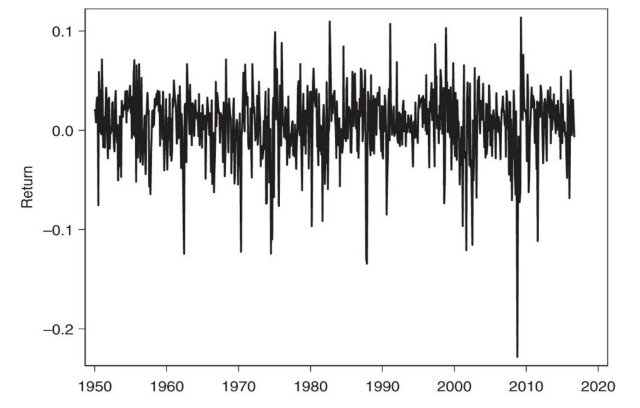
\includegraphics[width = 10cm]{pics/logreturn.png}
    \caption{Log Returns given lop price is linear}
    \label{fig:log return}
\end{figure}

We use the notation $r_t$ for log returns. 
\[ r_t = \log(1+R_t) = \log P_t - \log P_{t-1}\]

Over 2 periods:
\begin{align*}
    r_t(2) &= \log P_t - \log P_{t-2} \\
    &= (\log P_t - \log P_{t-1}) + (\log P_{t-1} - \log P_{t-2}) \\
    &= r_t + r_{t-1}
\end{align*}

Over $k$ periods:
\begin{align*}
    r_t(k) &= \log P_t - \log P_{t-k} \\
    &= (\log P_t - \log P_{t-1}) + (\log P_{t-1} - \log P_{t-2}) + \ldots +  (\log P_{t-k+1} - \log P_{t-k})\\
    &= \sum_{j=0}^{k-1} r_{t-j}
\end{align*}

\begin{note}
    the k-period log return is simply the sum of the single period log returns over the relevant periods. To annualise the monthly log returns we simply multiplying by 12.
\end{note}

\subsubsection{Excess Returns}
\begin{shaded}
\textbf{Excess Returns}: the difference between the return on a a risky financial asset and the risk. 
\begin{align*}
    \text{Simple Excess return } &= R_t - r_{ft} \\
    \text{Log Excess Return } &= r_t - r_{ft}
\end{align*}
\begin{note}
    We must ensure our returns are in the same units as the risk free rate of return. The risk free rate of return is usually expressed as an annual rate, therefore we can divide it my 12 when comparing monthly log returns.
\end{note}
\end{shaded}

\subsubsection{Portfolio Returns}

\begin{equation}
\begin{array}{lll}
\hline \text { Aggregation } & \text { Simple Return } & \text { Log Return } \\
\hline \text { Portfolio Return } & R_{P t}=\sum_{i=1}^N w_i R_{i t} & r_{P t}=\log \left(\sum_{i=1}^N w_i e^{r_{i t}}\right) \\
\text { K-Period Return } & R_{P t}(k)=\prod_{i=0}^{k-1}\left(1+R_{P t-i}\right)-1 & r_{P t}(k)=\sum_{i=0}^{k-1} r_{P t-i} \\
\hline
\end{array}
\end{equation}

\subsection{Stock Market Indices}

\begin{shaded}
    A stock market index is a summary measure of how well the stock market is doing as a whole. They are constructed in two main ways:
    \begin{enumerate}
        \item \textbf{Price-weighted} index: The weight given to each share is the price of the share. 
        e.g. Dow Jones, Nikkei 
        \item \textbf{Value-weighted} index: The weight given to each stock is proportional to the total market capitalisation.
        e.g. FTSE, S\&P 500, NASDAQ
    \end{enumerate}
\end{shaded}

\subsection{Statistical Properties of Financial Data}

\subsection*{Review of Statistical Methods}

\subsubsection*{Sum and Product}

A set of T observations on the variable $y$ given by $\{ y_1, y_2, \dots, y_T \}$
\[\sum_{t=1}^T y_t = y_1 + y_2 + \dots + y_T\]
\[\prod_{t=1}^{T} y_t = y_1 * y_2 * \dots * y_T\]


\subsubsection*{Expectation and Variance}

Let $Y$ be a discrete random variable which can take the values $(y_1, y_2, \ldots, y_T)$ with probability masses $f(y_1), f(y_2), \ldots, f(y_T)$. The expected value or expectation of Y, denoted $E(Y)$, is:
\[ E(Y) = \sum_{t=1}^T y_t f(y_t)\]

If Y is a continuous random variable with a probability density function (pdf) $f(Y)$, then 
\[E(Y) = \int_{-\infty}^\infty yf(y)\ dy\]

The variance of the random variable Y is:
\[ Var(Y) = E\left\{ [Y-E(Y)]^2 \right\} \]
 
\subsubsection*{Matrix Algebra}

The size of a matrix is described as \textbf{rows x columns}. If $A$ and $B$ are matrices of the same size, and $c$ is a scalar, then:

\begin{align*}
    A + B = C, &\text{ where } C_{i,j} = A_{i,j} + B_{i,j} \\
    cA = D, &\text{ where } D_{i,j} = cA_{i,j}
\end{align*}

Matrix multiplication:
\begin{equation*}
\underset{(M \times N)}{A} \times \underset{(N \times Q)}{B}=\underset{(M \times Q)}{C}
\end{equation*}

The elements of $C$ are computed as
\[ C_{ij} = \sum_{k=1}^N A_{ik}B_{kj}\]

Transposed Matrix $(A^T or A^\prime)$: Swapping rows and columns of a matrix. The $N \times N$ matrix is symmetric iff $A = A^\prime$

\subsubsection*{Differentiation}

Let f(y) denote a scalar function (i.e. returns one value) of the ($N \times 1$) vector
\begin{align*}
    y &= \begin{pmatrix}
    y_1 \\
    y_2\\
    \vdots \\
    y_N
    \end{pmatrix}
\end{align*}

The vector of partial derivatives, or the gradient vector, is also an $(N\times1)$ column vector given by 
\begin{equation}
\label{gradient vector}
G=\frac{\partial f}{\partial y}=\left(\begin{array}{c}
\frac{\partial f}{\partial y_1} \\
\frac{\partial f}{\partial y_2} \\
\vdots \\
\frac{\partial f}{\partial y_N}
\end{array}\right)
\end{equation}

The second derivative of $f$ with respect to each element in $y$ is given by the Hessian Matrix.

\begin{align*}
\label{hessian}
H=\frac{\partial^2 f}{\partial y \partial y^{\prime}}=\left(\begin{array}{ccccc}
\frac{\partial^2 f}{\partial y_1^2} & \frac{\partial^2 f}{\partial y_1 \partial y_2} & \frac{\partial^2 f}{\partial y_1 \partial y_3} & \cdots & \frac{\partial^2 f}{\partial y_1 \partial y_N} \\
\frac{\partial^2 f}{\partial y_2 \partial y_1} & \frac{\partial^2 f}{\partial y_2^2} & \frac{\partial^2 f}{\partial y_2 \partial y_3} & \cdots & \frac{\partial^2 f}{\partial y_2 \partial y_N} \\
\vdots & \vdots & \vdots & \ddots & \vdots \\
\frac{\partial^2 f}{\partial y_N \partial y_1} & \frac{\partial^2 f}{\partial y_N \partial y_2} & \frac{\partial^2 f}{\partial y_N \partial y_3} & \cdots & \frac{\partial^2 f}{\partial y_N^2}
\end{array}\right) \text {. }
\end{align*}

\subsubsection*{Distributions}
\begin{equation}
    \label{dist}
\end{equation}
\underline{Poisson distribution}: $f(y) = \dfrac{\lambda^y e^{-\lambda}}{y!}$, where $\lambda$ is both the mean and the variance of the distribution. \\

\noindent\underline{Normal distribution:}
\[f(y; \mu, \sigma^2) = \dfrac{1}{\sqrt{2\pi\sigma^2}}\exp{\left[ -\dfrac{(y-\mu)^2}{2\sigma^2}\right]}\] 
or $y \sim N(\mu, \sigma^2)$ \\

Let $\mathbf{X}=\left(X_1, X_2\right)^{\prime}$ be bivariate normal, with correlation $\rho$. The pdf of $\mathbf{X}$ is given by
$$
\begin{aligned}
&f\left(x_1, x_2\right)=  \frac{1}{2 \pi \sigma_1 \sigma_2 \sqrt{1-\rho^2}} \times \\
& \exp \left\{-\frac{1}{2 \sqrt{1-\rho^2}}\left[\frac{\left(x_1-\mu_1\right)^2}{\sigma_1^2}+\frac{\left(x_2-\mu_2\right)^2}{\sigma_2^2}-\frac{2 \rho\left(x_1-\mu_1\right)\left(x_2-\mu_2\right)}{\sigma_1 \sigma_2}\right]\right\} .
\end{aligned}
$$
If $\mathbf{X}$ is bivariate normal, then the marginal distribution (integrating out the other variable) of both $X_1$ and $X_2$ is: $X_1 \sim \mathcal{N}\left(\mu_1, \sigma_1^2\right)$ and $X_2 \sim \mathcal{N}\left(\mu_2, \sigma_2^2\right)$

\subsection{Characteristics of Financial Time Series Data}

\begin{enumerate}
    \item Heavy Tails (measured by kurtosis - 4th moment)
    \begin{itemize}
        \item The density of asset returns has heavier tails than normal
        \item There is excessively high proportion of extreme values
    \end{itemize}
    \item Asymmetry (measured by skewness - 3rd moment)
    \begin{itemize}
        \item The density of asset returns is slightly negatively skewed
        \item there is a higher proportion of negative returns than positive returns
    \end{itemize}
    \item Volatility clustering
    \begin{itemize}
        \item Large changes in log price come in clusters
        \item Can be seen in ARCH (autogressive conditional heteroskedasticity) literature
    \end{itemize}
    \item Departure from normality
    \begin{itemize}
        \item High frequency asset returns show obvious departure from normality
        \item The distribution of asset returns at other frequencies also tends to be non-normal
    \end{itemize}
    \item Long-range dependence (2nd order dependence)
    \begin{itemize}
        \item One observes strong serial correlation in variance of returns
        \item $r_t^2 or |r_t|$ is strongly autocorrelated
        \item This feature may help explain volatility clustering.
    \end{itemize}
    \item Log price of an asset is typically an integrated process
    \begin{itemize}
        \item Many such series appear to have upward trends
        \item These series commonly have unit roots, which affect inference
    \end{itemize}
    \item Some series of the log prices of assets keep co-movement in long run (can be seen as spurious relationship)
\end{enumerate}

Distributions that have a sharp peak in the centre of the distribution AND have slightly heavier tails are said to be \textbf{leptokurtic}.

\begin{figure}[h]
    \centering
    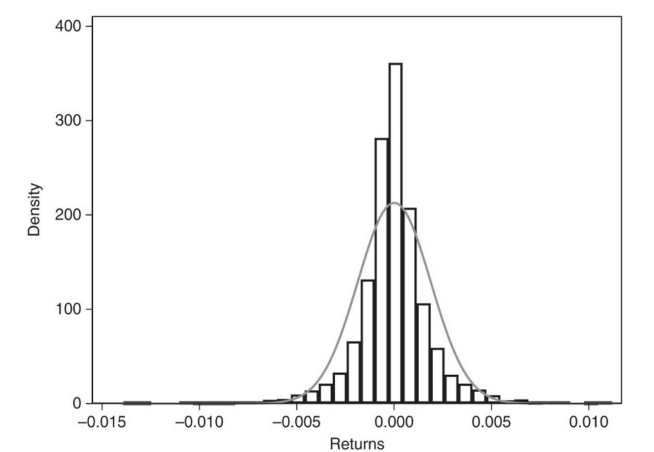
\includegraphics[width = 10cm]{pics/leptokurtic.png}
    \caption{Distribution of hourly \$/\textsterling \ exchange rate returns}
    \label{fig:leptokurtic dist pound return}
\end{figure}

\subsection{Summary Statistics}

\begin{enumerate}
    \item \textbf{Mean} (1st Moment): $\Bar{r} = \dfrac{1}{T}\sum_{t=1}^T r_t$
    \item \textbf{Variance} (2nd Moment): $s^2 = \dfrac{1}{T}\sum_{t=1}^T (r_t-\Bar{r})^2$
    \item \textbf{Skewness} (3rd Moment): $\text{SK } = \dfrac{1}{T} \sum_{t=1}^T \left( \dfrac{r_t- \Bar{r}}{s} \right)^3$
    \item \textbf{Kurtosis} (4th Moment): $\text{KT } = \dfrac{1}{T}\sum_{t=1}^T \left( \dfrac{r_t- \Bar{r}}{s} \right)^4 $

    The kurtosis of a normal distribution is 3. By comparing to this value we can find a measure called "excess kurtosis": $\text{EXCESS KT } = \dfrac{1}{T}\sum_{t=1}^T \left( \dfrac{r_t- \Bar{r}}{s} \right)^4 - 3$.

    A distribution with positive excess kurtosis is leptokurtic.
\end{enumerate}

Volatility is an obviously useful summary statistic: 
\[s = \sqrt{\dfrac{1}{T}\sum_{t=1}^T (r_t - \Bar{r})^2}\].

This is the sample standard deviation equation.

\subsubsection{Bivariate Descriptive Statistics}

In a portfolio we must assess the relationships between assets to see if they are well matched. Sample covariance is a measure of co-movements between the returns on two assets, $r_{it}$ and $r_{jt}$,
\begin{equation*}
s_{i j}=\frac{1}{T} \sum_{t=1}^T\left(r_{i t}-\bar{r}_i\right)\left(r_{j t}-\bar{r}_j\right) .
\end{equation*}

Sample correlation:

\begin{equation*}
\begin{gathered}
c_{i j}=\frac{s_{i j}}{\sqrt{s_{i i} s_{i j}}}, \\
\text{where }
s_{i i}=\frac{1}{T} \sum_{t=1}^T\left(r_{i t}-\bar{r}_i\right)^2, \quad s_{i j}=\frac{1}{T} \sum_{t=1}^T\left(r_{j t}-\bar{r}_j\right)^2 .
\end{gathered}
\end{equation*}

\subsection{Percentiles and Value at Risk}

\begin{shaded}
    \textbf{Value at Risk} (VaR): At a given confidence level, the worst loss that won'e be exceeded over a certain period of time. The 1\% VaR for the next $h$ periods conditional on the information at time $T$ is the 1st percentile of expected trading revenue (+ or -) at the end of the next $h$ periods. This is computed in 3 different ways:

    \begin{enumerate}
        \item Historical simulation
        \item Variance Method (Assumes normal distribution. 

        $\text{VaR}(1\%) = \hat{\mu} - 2.33 \times \hat{\sigma}$

        \item Monte Carlo Simulation
    \end{enumerate}

    Example: 
    The daily 1\% VaR is \$30 million, meaning, there is a 1\% chance the bank will lose \$30 million or more after 1 day.
\end{shaded}

\subsection{Efficient Markets Hypothesis}
\begin{shaded}
The \textbf{Efficient Markets Hypothesis (EMH)} is the idea that the market cannot be "beaten". If true this implies:
\begin{itemize}
    \item The current price of an asset reflects all information available on the market.
    \item The current price provides no information regarding future asset movements.
    \item Future returns are completely unpredictable, given information on past returns.
    \item Traders cannot systematically use newly arriving information to make a profit.
    \item Conditional on all previous information, returns are completely random.
\end{itemize}
\end{shaded}

We can examine EMH through various methods. We will specifically look at variance ratios and autocorrelation.

\subsubsection*{Variance Ratios}

First we must assume that the variances of $r_1, r_2, \ldots, r_t$ are the same and do not depend on $t$ (homoskedastic). The variance of 1-period and the n-period returns are:

\begin{equation*}
s_1^2=\frac{1}{T} \sum_{t=1}^T\left(r_t-\bar{r}\right)^2, \quad s_n^2=\frac{1}{T} \sum_{t=1}^T\left(r_{n t}-n \bar{r}\right)^2
\end{equation*}

In which
\begin{align*}
    r_t &= \log P_t - \log P_{t-1} \\
    r_{nt} &= \log P_t - \log P_{t-n} = r_t + r_{t-1} + \ldots + t_{t-(n-1)}
\end{align*}
and $n\Bar{r}$ represents the sample mean of the n-period returns $r_{nt}$. \\

If there is no autocorrelation, the variance of n-period returns should equal $n$ times the variance of the 1-period returns. The variance ratio is:
\[VR_n = \dfrac{s_N^2}{ns_1^2}\],
and we have:
\begin{equation}
VR_n \begin{cases}=1 & \text { [No autocorrelation] } \\ >1 & \text { [Positive autocorrelation] } \\ <1 & \text { [Negative autocorrelation]. }\end{cases}
\end{equation}

\subsection{Autocorrelation in Financial Returns}

The strength of association between the current return, $r_t$, and the return on the same asset $k$ periods earlier $r_{t-k}$ is given by the autocorrelation function:

\begin{equation*}
\operatorname{acf}(k)=\frac{T^{-1} \sum_{t=k+1}^T\left(r_t-\bar{r}\right)\left(r_{t-k}-\bar{r}\right)}{T^{-1} \sum_{t=1}^T\left(r_t-\bar{r}\right)^2}
\end{equation*}

Similar to the correlation formula, but being applied to a variable and it's own lag rather than two different variables.

If returns exhibit no predictability, then there should be no autocorrelation. If returns exhibit any autocorrelation then this pattern can be exploited to predict future behaviour, and EMH is violated.


\subsubsection*{Limitations of Autocorrelation}

\begin{itemize}
    \item Not a universal measure of predictability
    \item can capture, at most, linear predictability of mean returns
    \item we can extend the concept of autocorrelation to measure predictability of higher moments such as variance, skewness or kurtosis
\end{itemize}

\subsubsection*{Autocorrelation in squared returns}

Applying the same approach with squared returns we get:
\begin{equation}
a c f^2(k)=\frac{T^{-1} \sum_{t=k+1}^T\left(r_t^2-\overline{r^2}\right)\left(r_{t-k}^2-\overline{r^2}\right)}{T^{-1} \sum_{t=1}^T\left(r_t^2-\overline{r^2}\right)^2} 
\end{equation}
where
\begin{equation*}
    \overline{r^2}=\frac{1}{T} \sum_{t=1}^T r_t^2
\end{equation*}

This measures the correlation between the \textit{variance} of returns at time $t$ and the variance of returns at time $t-k$. 
\begin{itemize}
    \item We could have a negligible $acf(k)$ and sizable $acf^2(k)$
    \item In this case the mean is not predictable but the variance is
    \item This does not violate EMH which is solely concerned about expected returns, not their variance or any higher moments.
\end{itemize}

\paragraph{Various powers} of autocorrelation can by computed, such as:
\[r_t^3, \quad r_t^4, \quad |r_t|, \quad |r_t|^\alpha\]

\section{Linear Regression Models}

\subsection{Simple Linear Regression}

\subsubsection{CAPM}
CAPM describes the risk characteristics of an asset in terms of $\beta$-risk, given by:
\[\beta = \dfrac{cov(r_{it} - r_{ft},r_{mt}-r_{ft})}{var(r_{mt}-r_{ft})}\]

where $r_{it} - r_{ft}$ is the excess return of asset $i$ and $r_{mt}-r_{ft}$ is the excess market return. Stocks and portfolios of stocks are classified as follows in terms of their degree of $\beta$-risk:

\begin{equation}
\begin{array}{lc}
\text { Aggressive: } & \beta>1 \\
\text { Benchmark: } & \beta=1 \\
\text { Conservative: } & 0<\beta<1 \\
\text { Uncorrelated: } & \beta=0 \\
\text { Imperfect Hedge: } & -1<\beta<0 \\
\text { Perfect Hedge: } & \beta=-1 .
\end{array}
\end{equation}

The benchmark $\beta=1$ would be the market return, and when $\beta=0$ this gives us the risk-free return.

\subsubsection{CAPM Estimation}

We use the linear regression model:
\[r_{it} - r_{ft} = \alpha + \beta(r_{mt}-r_{ft}) + u\]
to estimate our $\beta$ value. In this case, $u_t$ captures all additional movements in the dependent variable not predicted in the CAPM. We assume a zero conditional mean:
\[E[U_t|r_{mt}-r_{ft}] = 0\]

Our intercept $\alpha$ captures the average abnormal return to the asset given the relative risks. The slope parameter $\beta$ corresponds to the asset's $\beta$ risk.

When we talk about risk we are talking about the 2nd moment, variance. By taking expectations of the CAPM model we have:

\begin{equation}
\underbrace{\mathrm{E}\left[\left(r_{i t}-r_{f t}\right)^2\right]}_{\text {Total risk }}=\underbrace{\mathrm{E}\left[\left(\alpha+\beta\left(r_{m t}-r_{f t}\right)\right)^2\right]}_{\text {Systematic risk }}+\underbrace{\mathrm{E}\left(u_t^2\right),}_{\text {Idiosyncratic risk }}
\end{equation}

This relies on the zero conditional mean assumption. From this assumption, we have that the covariance between the error term and excess market returns is 0.

\textbf{Systematic} risk is a risk that is inherent to the entire market i.e. non-diversifiable. \textbf{Idiosyncratic} risk is diversifiable.

\subsubsection{Linear Regressions in General}

Our simple linear regression model is:
\begin{equation}
y_t=\alpha+\beta x_t+u_t .
\end{equation}
$u_t$ represents the movements in $y_t$ that are not explained by the model and it has the properties:
\begin{equation}
\label{conditions of the error term}
\begin{aligned}
\text{Zero mean: } & \mathrm{E}\left(u_t\right)  =0, \\
\text{Constant and finite variance: }& \mathrm{E}\left(u_t^2\right) =\sigma_u^2, \\
\text{Zero Autocorrelation: }& \mathrm{E}\left(u_t u_{t-j}\right) =0, \\
\text{Contemporaneous Exogeneity: }& \mathrm{E}\left(x_t u_t\right) =0 .
\end{aligned}
\end{equation}

If the first three of these conditions are satisfied, we call our error term \textit{white noise}.

Our zero mean condition implies that the additional movements in $y_t$ that are in excess od the movements predicted by CAPM balance out to be zero on average. $\boldsymbol{\alpha}$ is inherent to the asset and not time-dependent. \textit{Constant and finite variance} implies homoskedasticity.

Our zero autocorrelation condition implies that movements in $u_t$ are uncorrelated with previous or future movements. Autocorrelation would imply arbitrage opportunities and would violate the Efficient Market Hypothesis (EMH).

Contemporaneous exogeneity ensures that movements in the market $x_t$ are independent of other factors (manifesting in $u_t$) caused by non-market movements.

\begin{shaded}
\subsubsection{Scalar Estimation}

From our simple linear regression:
\begin{equation}
y_t=\alpha+\beta x_t+u_t .
\end{equation}

we have:
\begin{equation}
\begin{aligned}
 \widehat{\beta}&=\frac{T^{-1} \sum_{t=1}^T\left(y_t-\bar{y}\right)\left(x_t-\bar{x}\right)}{T^{-1} \sum_{t=1}^T\left(x_t-\bar{x}\right)^2} \\
 \widehat{\alpha}&=\bar{y}-\widehat{\beta} \bar{x} \\
 \operatorname{se}(\widehat{\alpha})&=\sqrt{\frac{\widehat{\sigma}_u^2 \sum_{t=1}^T x_t^2}{T \sum_{t=1}^T\left(x_t-\bar{x}\right)^2}}, \\
 \operatorname{se}(\widehat{\beta})&=\sqrt{\frac{\widehat{\sigma}_u^2}{\sum_{t=1}^T\left(x_t-\bar{x}\right)^2}}, \\
 \widehat{\sigma}_u^2&=\frac{1}{T} \sum_{t=1}^T\left(y_t-\widehat{\alpha}-\widehat{\beta} x_t\right)^2 .
\end{aligned}
\end{equation}
\end{shaded}

\subsection{Matrix Linear models}

If we define the following column vectors:
\begin{equation}
y=\left(\begin{array}{c}
y_1 \\
y_2 \\
\vdots \\
y_T
\end{array}\right), \quad \beta=\left(\begin{array}{c}
\beta_0 \\
\beta_1 \\
\vdots \\
\beta_k
\end{array}\right), \quad u=\left(\begin{array}{c}
u_1 \\
u_2 \\
\vdots \\
u_T
\end{array}\right), \quad \widehat{\beta}=\left(\begin{array}{c}
\widehat{\beta}_0 \\
\widehat{\beta}_1 \\
\vdots \\
\widehat{\beta}_k
\end{array}\right), \quad \widehat{u}=\left(\begin{array}{c}
\widehat{u}_1 \\
\widehat{u}_2 \\
\vdots \\
\widehat{u}_T
\end{array}\right) \text {, }
\end{equation}
and the following matrix:
\begin{equation}
X=\left(\begin{array}{cccc}
1 & x_{11} & \ldots & x_{1 K} \\
1 & x_{21} & \ldots & x_{2 K} \\
\vdots & \vdots & & \vdots \\
1 & x_{T 1} & \cdots & x_{T K}
\end{array}\right)
\end{equation}

the population multiple regression model is written in observation form as:
\begin{equation}
    y = \boldsymbol{X}\beta + u
\end{equation}

\subsubsection{Matrix rules}
There are a couple matrix rules we need to know
\begin{align*}
    (AB)^\prime &= B^\prime A^\prime \\
    A(BC) &= (AB)C
\end{align*}
Assume $a$ and $b$ are both $k\times 1$ vectors and $A$ is a symmetric matrix:
\begin{align}
    \dfrac{\partial a^\prime b}{\partial b} &= \dfrac{\partial b^\prime a}{\partial b} = a \\
    \dfrac{\partial b^\prime Ab}{\partial b} &= 2Ab = 2b^\prime A
\end{align}

\subsubsection{Matrix Least Squares Problem}
\textbf{This is an important section to remember the matrix algebra for.}

\begin{mdframed}
We want to minimise the sum of squared residuals to find the best OLS estimator. So first we find the sum of squared residuals, $\mathbb{S}$:
\begin{equation}
\begin{aligned}
\mathbb{S} & =\sum_{t=1}^T u_t^2=u^{\prime} u=(y-X \beta)^{\prime}(y-X \beta) \\
& =y^{\prime} y-y^{\prime} X \beta-\beta^{\prime} X^{\prime} y+\beta^{\prime}\left(X^{\prime} X\right) \beta \\
& =y^{\prime} y-2 y^{\prime} X \beta+\beta^{\prime}\left(X^{\prime} X\right) \beta .
\end{aligned}
\end{equation}
\begin{note}
    $y^{\prime}X\beta - \beta^{\prime}X^{\prime}y$ are both the same scalar transposed. A scalar transposed is still just the same scalar, meaning that we can sum these two terms together.
\end{note}

We want to find $\beta$ that minimises $\mathbb{S}$, so we take derivatives w.r.t. $\beta$:
\begin{equation}
\frac{\partial S}{\partial \beta}=0-2 X^{\prime} y+2\left(X^{\prime} X\right) \beta
\end{equation}
Then setting the derivative to zero yields:
\begin{equation}
-2 X^{\prime} y+2\left(X^{\prime} X\right) \widehat{\beta}=0 \Rightarrow\left(X^{\prime} X\right) \widehat{\beta}=X^{\prime} y
\end{equation}
By multiplyin gboth sides of the equation by $(X^\prime X)^{-1}$ we get:
\[\hat{\beta} = (X^\prime X)^{-1}X^\prime y\]

It can be shown that:
\begin{equation}
\operatorname{Var}(\widehat{\beta})=\sigma^2\left(X^{\prime} X\right)^{-1}
\end{equation}
\end{mdframed}

\begin{note}
    For $\left(X^{\prime} X\right)^{-1}$ to exist, we rely on the no perfect collinearity assumption
\end{note}


\subsubsection{Extensions of CAPM}
There are many extensions to the CAPM, zero-beta models, multi-factor models, time-varying $\beta$ models etc. 

\paragraph{Fama-French 3 factor model} \mbox{}

The Fama-French 3 factor model introduces two extra factors which are \textbf{SMB} (small minus big) and \textbf{HML} (high minus low).

\textbf{SMB} refers to the performance of big stocks versus that of small stocks. Size refers to market cap. This comes from the observation that firms with small market caps outperformed large market cap firms. SMB accounts for the spread in returns between small- and large-sized firms. Including this in our model shows whether management/investors are relying on the small firm effect to earn an abnormal return.

\textbf{HML} is the additional factor which captures the performance of "value" stocks relative to growth stocks.
\begin{itemize}
    \item Value stocks: companies with \textbf{high} book-to-market ratios
    \item Growth stocks: companies with \textbf{low} book-to-market ratios
\end{itemize}

Book to the market ratio: book value of the firm divided by the market value of the firm. The book value is calculated by looking at the firm's historical cost, or accounting value. Market value is a firm's market cap.

So the Fama-French 3-factor model can be shown as:
\begin{equation}
r_{i t}-r_{f t}=\alpha+\beta_1\left(r_{m t}-r_{f t}\right)+\beta_2 \mathrm{SMB}_t+\beta_3 \mathrm{HML}_t+\epsilon_t .
\end{equation}

where,
\begin{equation}
\begin{aligned}
\text { SMB } & =1 / 3 \text { (Small Value + Small Neutral + Small Growth) } \\
& -1 / 3 \text { (Big Value + Big Neutral + Big Growth) }
\end{aligned}
\end{equation}
and
\begin{equation}
\begin{aligned}
\mathrm{HML} & =1 / 2 \text { (Small Value }+ \text { Big Value) } \\
& -1 / 2 \text { (Small Growth + Big Growth) }
\end{aligned}
\end{equation}

The different categories are split:
\begin{figure}[h]
    \centering
    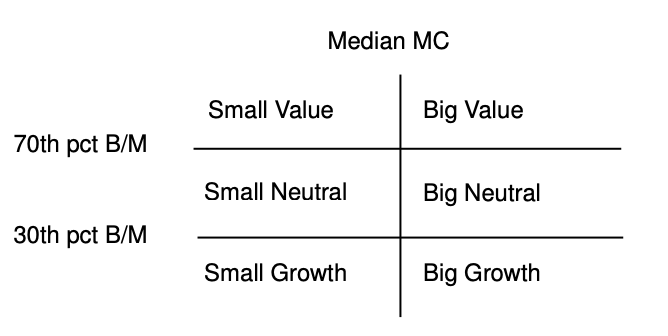
\includegraphics[width=8cm]{pics/ff3.png}
    \caption{Categorisation of firms in Fama-French 3 Factor model}
    \label{fig:ff3}
\end{figure}



\begin{mdframed}
    Results:
    \begin{itemize}
        \item For $\beta_2$ estimated greater than 0.5, this signifies a portfolio composed mainly of small-cap stocks, and a zero value signifies large-cap stocks
        \item $\beta_3$ being greater than 0.3 signifies a portfolio composed mainly of value stocks.
    \end{itemize}
\end{mdframed}
These categories are not fixed. If one were to create a model based on this framework, one could add more factors, separating market cap into 3 sections as well. You could as other factors like Robust Minus Weak (RMW), Conservative Minus Aggressive (CMA) or momentum.

\subsection{Diagnostics}

So far we have assumed our models are correctly specified, but we might have omitted factors and misspecified the model.

These diagnostic procedures are categorised into three categories involving diagnostics on the dependent variable $y_t$, the explanatory variables $\{x_{1t}, x_{2t},\ldots, x_{kt}\}$, and the disturbance term $u_t$.

\paragraph{$\boldsymbol{R^2}$} \mbox{}


The $R^2$ tells us the proportion of the variation in the dependent variable that is explained by the model. This is also called the coefficient of determination.

\begin{equation}
R^2=\frac{\text { Explained SS }}{\text { Total SS }}=1-\frac{\text { Unexplained SS }}{\text { Total SS }}
\end{equation}

\begin{note}
    Variation is equivalent to the sum of squares (SS)
\end{note}

The proportion of variation in the dependent variable explained by the explanatory variables

\begin{equation}
R^2=\frac{\text { systematic risk }}{\text { total risk }}=1-\frac{\text { idiosyncratic risk }}{\text { total risk }}
\end{equation}

When we want to compare models with different numbers of explanatory variables we must use an \textbf{adjusted} $R^2$, denoted $\bar{R}^2$.

\begin{equation}
\bar{R}^2=1-\left(1-R^2\right) \frac{T-1}{T-K-1}
\end{equation}

There is a penalty adjustment for the additional model parameters $K$. You will always increase the $R^2$ when you add additional explanatory variables, but you can increase or \textit{decrease} the $\Bar{R}^2$.

When there is a low $R^2$ it does not necessarily imply misspecification, it could just be that the data is noisy. An $R^2$ lower than 5\% is common, according to EMH there is no effective predictor of future returns.

However, when the $R^2$ is very small we tend to look to the tests concerning the disturbance term $u_t$. If the model is correctly specified, then we would not expect any information in $u_t$.

\paragraph{t-test} \mbox{}

The t-test is a single-parameter test:
\begin{mdframed}
Consider:
\begin{equation}
y_t=\alpha+\beta_1 x_{1 t}+\beta_2 x_{2 t}+\ldots+\beta_K x_{K t}+u_t
\end{equation}
    The t-test test the null hypothesis:
    \begin{align*}
        H_0: \beta &= c \\
        H_1: \beta &\neq c
    \end{align*}

    We have:
    \begin{equation}
\text { Test statistic and distribution: } \quad t=\frac{\hat{\beta}-c}{\operatorname{se}(\hat{\beta})} \sim t_{T-K-1}
\end{equation}
\end{mdframed}

We can also use the t-test for parameter significance:
\begin{mdframed}
    \begin{align*}
        H_0&: \beta = 0 \\
        H_1&: \beta \neq 0
    \end{align*}
    \begin{equation}
\text { Test statistic and distribution: } \quad t=\frac{\hat{\beta}}{\operatorname{se}(\hat{\beta})} \sim t_{T-K-1}
\end{equation}
\end{mdframed}

\paragraph{Joint Parameter Test} \mbox{}

The joint parameters tests, test the following null and alternative hypotheses.

$H_0:$ list of restrictions on the model parameters

$H_1:$ at least one of the listed restrictions does not hold.

These compare a restricted and unrestricted model and compare the two via their residual sum of squares values.

\begin{mdframed}
Test statistic and distribution: $\quad J=\frac{R S S_0-R S S_1}{R S S_1 /(T-K-1)} \sim \chi_R^2$
    
$\underset{\text { (Small samples) }}{\text { Test statistic and distribution: }} \quad F=\frac{\left(R S S_0-R S S_1\right) / R}{R S S_1 /(T-K-1)} \sim F_{R, T-K-1}$

where $K$ is the number of explanatory variables in the unrestricted model and $R$ is the number of restrictions listed in $H_0$.
\end{mdframed}

\paragraph{Testing for overall model significance} \mbox{}

Consider the same model specification:
\begin{equation}
y_t=\alpha+\beta_1 x_{1 t}+\beta_2 x_{2 t}+\ldots+\beta_K x_{K t}+u_t
\end{equation}

We can test:

$H_0: \beta_1 = \beta_2 = \ldots = \beta_k = 0$ i.e. all slope parameters are zero.

$H_1:$ at least one of the slopes is nonzero.

other forms of linear restrictions:

$H_1: \beta_1=1$ and $\beta_2 + \beta_k=0$
$H_1:$ at least one of the restrictions listed above does not hold.

\paragraph{Disturbance Diagnostics} \mbox{}

If the model is correctly specified, there should be no information in the error term. That is:

$H_0: u_t$ is random (model is correctly specified)

$H_1: u_t$ is not random (model is misspecified)

in our linear regressions, we made crucial assumptions about the error term \eqref{conditions of the error term}. Namely:

\begin{align*}
    E(u_tu_{t-j}) &= 0, j\neq0 \text{ no autocorrelation} \\
    E(U_t^2) &= \sigma^2 \text{ constant variance }
\end{align*}

The diagnostics on the disturbance term are concerned with its mean (autocorrelation), variance (heteroskedasticity) and distributional shape (normality).

\paragraph{Autocorrelation} \mbox{}

When there is autocorrelation in the error term it effects the efficiency of our estimator and therefore it is no longer the best estimator. That is why we want to test for autocorrelation.

To test for autocorrelation in the disturbance term we use the Breusch-Godfrey test.

\begin{mdframed}
    $H_1:$ No autocorrelation in the disturbances

    $H_1:$ Autocorrelation up to lag $p$ in the disturbances

    \[\text{Test statistic and distribution: } AR(p) \sim \chi_p^2\]

    where $p$ is the autocorrelation lag length tested.
\end{mdframed}

What we are doing with this test is estimating:

\begin{equation}
y_t=\alpha+\beta_1 x_{1 t}+\beta_2 x_{2 t}+\ldots+\beta_K x_{K t}+u_t
\end{equation}

and getting the residuals $\hat{u}_t$. Then we test if the residuals have autocorrelation up to lag $p$, by estimating:

\begin{equation}
\hat{u}_t=\gamma_0+\gamma_1 x_{1 t}+\gamma_2 x_{2 t}+\ldots+\gamma_K x_{K t}+\rho_1 \hat{u}_{t-1}+\rho_2 \hat{u}_{t-2}+\ldots+\rho_p \hat{u}_{t-p}+v_t
\end{equation}

and running a test on the joint restriction:

$H_1: \rho_1=\rho_2=\ldots=\rho_p=0$

\[\text{Test statistic and distribution: } AR(p) = TR^2 \sim \chi_p^2\]

where $R^2$ is the coefficient of determination from the second regression and $T$ is the sample size from the second regression.

It is worth noting there is also a Durbin-Watson test which tests for autocorrelation in the errors, but only first-order autocorrelation. The Godfrey test is a more diverse and applicable test.

\paragraph{Heteroskedasticity} \mbox{}

Again, when there is heteroskedasticity in our error terms, it is no longer the most efficient and therefore no longer the best estimator. However, in both cases (autocorrelation included) the estimator is still consistent and unbiased.

To test for heteroskedasticity we use \textbf{White's} test.

\begin{mdframed}
    $H_0:$ Homoskedastic disturbances ($\sigma_u^2$ is constant)

    $H_1:$ Heteroskedastic disturbances ($\sigma_u^2$ is time-varying)

    \[\text{Test statistic and distribution: } HSK \sim \chi_k^2\]

    where $k$ is the number of explanatory regressors in the auxiliary regression
\end{mdframed}

Again, to actually do this we need to estimate the regressors as we did with autocorrelation. We want to test if the variance of the residuals is influenced by the explanatory variables. We use the squared residuals as a proxy for this.

We run the auxiliary regression:

\begin{equation}
\begin{aligned}
\hat{u}_t^2= & \gamma_0+\gamma_1 x_{1 t}+\gamma_2 x_{2 t}+\ldots+\gamma_K x_{K t} \\
& +\gamma_{K+1} x_{1 t}^2+\gamma_{K+2} x_{2 t}^2+\ldots+\gamma_{K+K} x_{K t}^2 \\
& +\gamma_{2 K+1} x_1 x_2+\left(\begin{array}{c}
\text { all bivariate combinations } \\
\text { of regressors }
\end{array}\right)+v_t
\end{aligned}
\end{equation}

and test:

$H_0: \gamma_1 = \gamma_2 = \ldots = \gamma_m = 0$ (excluding $\gamma_0$)

\[\text{Test statistic and distribution: } HSK = TR^2 \sim \chi_m^2\]

where $R^2$ is the coefficient of determination from the second regression and $m$ is the number of explanatory regressors in the auxiliary regression.

\[m = kC2 = \dfrac{k(k-1)}{2}\]

\paragraph{ARCH} \mbox{}

AutoRegressive Conditional Heteroskedasticity - volatility (variance) clustering. This implies that low variance follows low variance and high variance follows high variance.

\begin{mdframed}
    ARCH test:

    $H_0:$ no ARCH in disturbances

    $H_1:$ ARCH of order $p$ in disturbances

    \[\text{Test statistic and distribution: } ARCH(p) = TR^2 \sim \chi_p^2\]

    where $p$ is the order of ARCH tested.
\end{mdframed}

Again we must get the residuals from the original regression, $\hat{u}_t$. We then run the auxiliary regression:
\begin{equation}
    \hat{u}_t^2=\gamma_0+\gamma_1 \hat{u}_{t-1}^2+\gamma_2 \hat{u}_{t-2}^2+\ldots+\gamma_p \hat{u}_{t-p}^2+v_t
\end{equation}

and test

$H_0: \gamma_1 = \gamma_2 = \ldots = \gamma_p = 0$

\[\text{Test statistic and distribution: } ARCH(p) = TR^2 \sim \chi_p^2\]

Again $R^2$ is the coefficient of determination from the second regression and $T$ is the sample size in the second regression. 

\paragraph{Normality} \mbox{}

\begin{mdframed}
    Normality test:

    $H_0:$ disturbances are normally distributed

    $H_1:$ disturbances are not normally distributed

    \[\text{Test statistic and distribution: } J B =T\left(\frac{S K^2}{6}+\frac{(K T-3)^2}{24}\right) \sim \chi_2^2\]
\end{mdframed}

\begin{note}
    this is a test of both skewness and kurtosis together.
\end{note}

Calculate the skewness and kurtosis of the disturbances:

\[SK = \dfrac{1}{T} \sum_{i=1}^T \left(\dfrac{\hat{u}_t}{\hat{\sigma}_u}\right)^3 \qquad KT = \dfrac{1}{T} \sum_{i=1}^T \left(\dfrac{\hat{u}_t}{\hat{\sigma}_u}\right)^4\]

We expect $SK=0, KT=3$ if the disturbances come from a normal distribution.

 \[\text{Test statistic and distribution: } J B =T\left(\frac{S K^2}{6}+\frac{(K T-3)^2}{24}\right) \sim \chi_2^2\]

 \subsection{Event Analysis}

 Used to model the effect of qualitative changes on financial variables arising from a discrete event. The event is decomposed into \textbf{three sub-events}: the part anticipated by the market, the part that occurs at the time of the event, and the part that happens after the event has occurred.

 \paragraph{Dummy/indicator Variables} parameters have the interpretation of the \textit{abnormal} return associated with the event, representing the return over and above the normal return.

 If we were to add indicator variables 3 months on either side of the event date, we would be able to test whether the market anticipated/ reacted to the event in a significant way.

 We could estimate the following model:

 \begin{equation}
\begin{aligned}
r_t & =\underbrace{\beta_0+\beta_1 r_{m t}}_{\text {Normal return }} \\
& +\underbrace{\delta_{-2} I_{\text {Oct }, t}+\delta_{-1} I_{\text {Nov }, t}+\delta_0 I_{\text {Dec }, t}+\delta_1 I_{\text {Jan }, t}+\delta_2 I_{\text {Feb }, t}}_{\text {Abnormal return }}+u_t .
\end{aligned}
\end{equation}

we get the following results:
\begin{equation}
\begin{aligned}
r_t & =\underset{(0.002)}{0.009}+\underset{(0.044)}{0.651} r_{m t}-\underset{(0.041)}{0.121} I_{O c t, t}+\underset{(0.041)}{0.007} I_{\text {Nov }, t} \\
& -\underset{(0.041)}{0.041} I_{\text {Dec }, t}+\underset{(0.041)}{0.086} I_{\text {Jan }, t}-\underset{(0.041)}{0.059} I_{F e b, t}+\widehat{u}_t .
\end{aligned}
\end{equation}

We can see that the market viewed the event unfavourably. The net effect of the event on the market was negative with the total abnormal return equalling:

\[\text{total } = -0.121 + 0.007 - 0.041 + 0.086 - 0.059 = -.0128\]

We then can run a joint test of the hypothesis:

$H_0: \quad \delta_{-2}=\delta_{-1}=\delta_0=\delta_1=\delta_2=0 \quad$ [Normal returns]

$H_1$: at least one restriction is not valid [Abnormal returns].

Under the null hypothesis, the regression model reduces to the simple CAPM.

\subsection{Minimum Variance Portfolio}

A common goal in choosing a portfolio of assets is to minimise the overall risk of the portfolio, measured in variance (squared volatility).

Consider a portfolio consisting of 2 assets:
\begin{shaded}
    

Mean: $\quad \mu_1=E\left[r_{1 t}\right], \quad \mu_2=E\left[r_{2 t}\right]$,

Variance: $\quad \sigma_1^2=E\left[\left(r_{1 t}-\mu_1\right)^2\right], \quad \sigma_2^2=E\left[\left(r_{2 t}-\mu_2\right)^2\right]$,

Covariance: $\quad \sigma_{12}=E\left[\left(r_{1 t}-\mu_1\right)\left(r_{2 t}-\mu_2\right)\right]$.

The return on the portfolio is:
\[r_{pt} = w_1r_{1t} + w_2 r_{2t}, \qquad w_1 + w_2 = 1\]

The expected return on this portfolio is:

\begin{equation}
\mu_p=E\left(w_1 r_{1 t}+w_2 r_{2 t}\right)=w_1 E\left(r_{1 t}\right)+w_2 E\left(r_{2 t}\right)=w_1 \mu_1+w_2 \mu_2
\end{equation}

A measure of portfolio risk is given by the \textbf{variance}:
\begin{equation}
\sigma_p^2=E\left[\left(r_{p t}-\mu_p\right)^2\right]=w_1^2 \sigma_1^2+w_2^2 \sigma_2^2+2 w_1 w_2 \sigma_{12}
\end{equation}
\end{shaded}

\begin{mdframed}
    \textbf{The portfolio problem:}

    Portfolio risk can be re-expressed as

    \begin{equation}
\sigma_p^2=w_1^2 \sigma_1^2+\left(1-w_1\right)^2 \sigma_2^2+2 w_1\left(1-w_1\right) \sigma_{12}
\end{equation}

with the optimisation problem as

\[\underset{w_1}{\text{min}}\sigma_p^2\]

We can differentiate our re-expressed risk w.r.t. $w_1$ and solve;

\begin{equation}
w_1=\frac{\sigma_2^2-\sigma_{12}}{\sigma_1^2+\sigma_2^2-2 \sigma_{12}}, \quad w_2=\frac{\sigma_1^2-\sigma_{12}}{\sigma_1^2+\sigma_2^2-2 \sigma_{12}}
\end{equation}

solving for $w_1$ gives us $w_2$ as well as they sum to 1.

What we find is that the minimum variance weights are a function of the returns variances $\sigma_1^2$ and $\sigma_2^2$ and the covariance $\sigma_{12}$.
\end{mdframed}

\subsection{Portfolio Performance Measures}

The three well known measures of a portfolio's performance are
\begin{enumerate}
    \item Sharpe Ratio
        \[S = \dfrac{\mu_p - r_f}{\sigma_p}\]

        \begin{itemize}
            \item Considers both systematic and idiosyncratic risks
            \item does not quantify the value added compared to the market return
            \item we must assume that returns are normally distributed (because lots of financial returns show leptokurtic distributions this Sharpe ratio will be positively biased)
            \item Penalises upside volatility, Sortino only penalises downside volatility.
        \end{itemize}

    \item Treynor Index
        \[T = \dfrac{\mu_p - r_f}{\beta}\]

        \begin{itemize}
            \item also does not quantify the value added relative to the market
            \item considers only systematic risk since $\beta$ is in the denominator
            \item portfolios with identical systematic risk, but different total risk will be rated the same.
        \end{itemize}

    \item Jensen's Alpha
        \[\alpha = \mu_p - r_f -\beta(\mu_m - r_f)\]

        \begin{itemize}
            \item quantifies the added return as the excess return above that predicted by CAPM
            \item rankings done on Jensen's alpha only take into account systematic risk, so it will rank portfolios in a similar way to the Treynor Index.
        \end{itemize}
\end{enumerate}
where $\mu_p$ and $\mu_m$ are respectively the expected returns on the portfolio and the market. In all cases we want these values to be the largest they can be.


\section{Instrumental Variables}
\textbf{Chapter 8}
\subsection{Exogeneity Condition}
In our simple regression model, we have 
\[y_t = \beta_0 + \beta_1 x_t + u_t\]

Our exogeneity condition, also known as the orthogonality condition, is expressed as:
\[E(u_tx_t)=0\]
This is equivalent to 
\[E[u_t|x_t] = 0\]
when we have a zero mean. This assumption is often violated by the following situations:

\begin{enumerate}
    \item Errors in variable
    \item Omitted Variables
    \item Simultaneous causality
\end{enumerate}

in the simple CAPM we have:
\[r_{it} - r_{ft} = \alpha + \beta(r_{mt}-r_{ft})+ u_t\]
and the orthogonality condition is:
\[E[u_t|r_{mt}-r_{ft}] = 0.\]

This is obviously not a very realistic assumption. This is saying that unobserved shocks to the market are uncorrelated with excess market returns.

\paragraph{Dealing with Endogeneity} can be done through a method called \textbf{Instrumental Variable Estimation}. These instrumental variables (IV) must be \hl{relevant and exogenous}.

\paragraph{Instrument Relevance} means that the valid instrument, $z_t$, is correlated with the endogenous explanatory variable in the regression:
\[Cov(z_t, x_t)\neq0\]
When variables are endogenous, as $x_t$ is, it is difficult to establish causality.

\paragraph{Instrument Exogeneity} means that $z_t$ must be uncorrelated/orthogonal to the regression equation disturbances:
\[Cov(z_t,u_t)=0\]

\begin{note}
    It is possible for there to be more instruments, $z_t$, than endogenous variables, $x_t$.
\end{note}

\subsection{Inter-temporal CAPM}

Investors need higher excess returns as the stock market gets riskier. We can estimate the risk-return tradeoff using th CAPM. The way to capture this relationship is:
\[E_{t-1}(r_t) = \gamma E_{t-1}(\sigma^2_t)\]
The subscripts mean that the expectations are based on information at time $t-1$. Excess return on the aggregate stock market at time $t, r_t,$ is a linear function of the expected variance at time $t, \sigma^2$.

\paragraph{Building the Model}

We take this relationship and model it using linear regression:
\begin{equation}
    \label{intertemporal CAPM}
    r_t = \alpha + \gamma E_{t-1}(\sigma^2_t) + u_t
\end{equation}

Equation \eqref{intertemporal CAPM} is known as the inter-temporal CAPM. When the parameters satisfy the restrictions $\alpha=0,\gamma>0$, it is called the Merton model.

We must observe $E_{t-1}(\sigma_t^2)$ to estimate this model. The best way to do this is to use a proxy because the expected conditional variance is unobservable. The \textbf{VIX} is an index for the volatility of the S\&P 500 stock market index.

The relationship between the proxy variance, $h_t$ (VIX), and the true unobserved conditional variance is:
\[h_t = E_{t-1}(\sigma_t^2) + \epsilon_t, \qquad \epsilon_t \sim i.i.d(0,\sigma_\epsilon^2)\]

The inter-temporal CAPM then becomes:
\[t_t = \alpha+ \gamma h_t + v_t\]
with \[v_t = -\gamma \epsilon_t + u_t\]

Assuming $\epsilon_t$ and $u_t$ are independent, the covariance of $h_t$ and $v_t$ is:
\[cov(h_t,v_t) = cov[E_{t-1}(\sigma_t^2) + \epsilon_t),(-\gamma \epsilon_t + u_t)] = -\gamma \sigma_\epsilon^2 \neq 0\]

Exogeneity is violated. When there is measurement error $\sigma_\epsilon^2\neq0$, the slope parameter is biased downward. This implies the least squares produce an inconsistent estimator of $\gamma$. We can see this from the equation for the slope parameter in the inter-temporal CAPM below:

\begin{equation}
\frac{\operatorname{cov}\left(r_t, h_t\right)}{\operatorname{var}\left(h_t\right)}=\frac{\operatorname{cov}\left(\alpha+\gamma h_t+v_t, h_t\right)}{\operatorname{var}\left(h_t\right)}=\gamma+\frac{\operatorname{cov}\left(v_t, h_t\right)}{\operatorname{var}\left(h_t\right)}=\gamma-\gamma \frac{\sigma_\epsilon^2}{\operatorname{var}\left(h_t\right)}
\end{equation}

The estimated slope parameter, $\hat{\gamma}=\gamma$ only when $\sigma_\epsilon^2=0$.

A higher $\gamma$ implies a higher level of risk aversion because a downward bias means lower risk aversion. The model tells us investors are less risk-averse than they actually are.

\subsection{Simple Instrumental Estimator}

Suppose we have a valid instrument, $z_t$ that satisfies our relevance and exogeneity conditions. Then the covariance between returns, $r_t$ and the variable, $z_t$, id given by
\begin{equation}
\begin{aligned}
\operatorname{cov}\left(r_t, z_t\right) & =\operatorname{cov}\left(\alpha+\gamma h_t+v_t, z_t\right) \\
& =\operatorname{cov}\left(\gamma h_t, z_t\right)+\operatorname{cov}\left(v_t, z_t\right) \\
& =\gamma \operatorname{cov}\left(h_t, z_t\right)
\end{aligned}
\end{equation}
By rearranging the expression we see an alternative version of the population parameter $\gamma$:
\begin{equation}
\gamma=\frac{\operatorname{cov}\left(r_t, z_t\right)}{\operatorname{cov}\left(h_t, z_t\right)}
\end{equation}

When we replace the population quantities with the sample counterparts, we have the \textbf{simple instrumental variable estimator}:

\begin{equation}
\widehat{\gamma}_{I V}=\frac{\frac{1}{T} \sum_{t=1}^T\left(r_t-\bar{r}\right)\left(z_t-\bar{z}\right)}{\frac{1}{T} \sum_{t=1}^T\left(h_t-\bar{h}\right)\left(z_t-\bar{z}\right)}
\end{equation}

Given $z_t$ is a valid instrument, $\gamma_{IV}$ is a consistent estimator of $\gamma$

\subsubsection{How do we estimate?}

\begin{procedure}
To consistently estimate:
\begin{equation}
    \label{structural iv}
    r_t =\alpha + \gamma h_t + v_t
\end{equation}

we use \textbf{two-stage least squares}.

In the first stage, we estimate:
\begin{equation}
    \label{iv first stage}
    h_t = \pi_0 + \pi_1 z_t + e_t
\end{equation}
by OLS and compute predicted values for $\hat{h}_1, \ldots, \hat{h}_N$. 

In the second, we estimate:
\begin{equation}
    \label{iv second stage}
    r_t = \alpha + \gamma \hat{h}_t + v_t
\end{equation}
using OLS to obtain $\hat{\gamma}_{IV}$. The resulting estimator is a special case of \textit{generalised least squares estimator}.
\end{procedure}

Equation \eqref{structural iv} is called a \textbf{Structural equation}. 
\begin{definition}
\textbf{Structural Equation}: describes some aspect of the "structure" of the economy or market.

They:
\begin{itemize}
    \item  Carry behavioural content (e.g. how investors react to risk)
    \item Typically are of the greatest interest to the modeller
    \item Can contain $\geq 1$ endogenous regressors, and cannot be consistently estimated by OLS.
\end{itemize}

A structural equation is said to be \textbf{identified} if there is at least one instrument available for each endogenous regressor. If there are fewer instruments (\textit{unidentified)}, the parameters cannot be consistently estimated. If there are more instruments (\textit{overidentified}), that's fine.
\end{definition}

Equation \eqref{iv first stage} is called a \textbf{reduced form equation}

\begin{definition}
    \textbf{Reduced Form Equation:} expresses an endogenous variable exclusively in terms of exogenous variables. 
    They:
    \begin{itemize}
        \item Can be consistently estimated by OLS
        \item Do not carry any behavioural interpretations.
    \end{itemize}
\end{definition}

\newpage

\begin{example}
\item
\paragraph{Instrument for Inter-temporal CAPM} \mbox{}

Back to inter-temporal CAPM. What could we use for an instrument, $z_t$, for the VIX, $h_t$? We can use the first lag of VIX, $h_{t-1}$.

The reason is that at time $t$, the lagged value $h_{t-1}$ can be taken as given, therefore it is uncorrelated with the random variable $v_t \Rightarrow cov(h_{t-1}, v_t)=0$. It is also \textit{highly correlated} with $h_t$ because of first-order autocorrelation and hence $cov(h_t, h_{t-1}) \neq 0.$

Using returns on S\&P 500 as $r_t$, the \textbf{structural estimates} are:
\[\hat{r}_t = \underset{(0.0002)}{0.0018} - \underset{(0.9534)}{9.7202}h_t\]

The negative risk-aversion parameter suggests that investors require lower returns when markets are riskier. It defies the theory of the risk-return relationship.

The \textbf{IV estimates} are:
\[\hat{r}_t = -\underset{(0.0002)}{0.0003} + \underset{(0.9975)}{3.0190}\hat{h}_t\]

The risk aversion parameter indicates that investors require more returns when the market is more volatile. This has a \textit{downward bias}. This coefficient can be interpreted as: an increase in 1 standard deviation in variance, investors need a 302\% increase in returns.
\end{example}

\subsection{General Instrumental Variable Estimator}

Suppose there are $N$ endogenous variables, $x_{1t}, \ldots, x_{Nt}$ and K exogeneous variables, $w_{1t}, \ldots, w_{Kt}$, so that the model is specified as:

\begin{equation}
y_t=\beta_0+\sum_{i=1}^N \beta_i x_{i t}+\sum_{i=k}^K \phi_k w_{k t}+v_t .
\end{equation}

\begin{procedure}
    The General IV estimator is computed as follows:
    \begin{enumerate}
        \item Estimate the \textbf{reduced form}

        \begin{equation}
x_{i t}=\pi_{i 0}+\sum_{j=1}^L \pi_{i j} z_{j t}+\sum_{k=1}^K \psi_{i k} w_{k t}+e_{i t}, \quad i=1,2, \cdots, N .
\end{equation}

by OLS and compute the predicted values $\hat{x}_{1t},\ldots, \hat{x}_{Nt}$. 

\begin{note}
    We included $w_{Kt}$ to retain as much information for the computation of $\hat{x}_t$. If we include control variables in the structural equation, we want them in the first stage reduced form estimation.
\end{note}

\item Estimate:
\begin{equation}
y_t=\beta_0+\sum_{i=1}^N \beta_i \widehat{x}_{i t}+\sum_{k=1}^K \phi_k w_{k t}+v_t
\end{equation}
by OLS to obtain the estimator $\hat{\theta}_{IV} = \{\hat{\beta}_0, \ldots, \hat{\beta}_N, \hat{\phi}_1, \ldots, \hat{\phi}_K\}$.
    \end{enumerate}
\end{procedure}

Let $X$ be a $(T\times N)$ matrix of endogenous variables, and $Z$ be a $(T\times L)$ matrix of exogenous variables. It can be shown that
\begin{equation*}
\hat{\beta}_{I V}=\left(X^{\prime} P_z X\right)^{-1} X^{\prime} P_z y
\end{equation*}

where $P_z=Z\left(Z^{\prime} Z\right)^{-1} Z^{\prime}$.

\begin{proof}
In our first stage regression we have:
\[\underset{(T \times N)}{X}=\underset{(T \times L)}{Z} \underset{(U \times N)}{\Pi} \underset{(T \times N)}{\epsilon}\]
From the OLS derivation we know:
\begin{equation}
\underset{(L \times N)}{\hat{\Pi}}=\left(\underset{(L \times T)}{Z^{\prime}} \underset{(T \times L)}{Z} \right)^{-1} \underset{(L \times T)}{Z^{\prime}}\underset{(T \times N)}{X}
\end{equation}
and hence:
\begin{equation}
\hat{X}=Z \hat{\Pi}=Z\left(Z^{\prime} Z\right)^{-1} Z^{\prime} X \equiv P_Z X
\end{equation}
where $P_Z=Z\left(Z^{\prime} Z\right)^{-1} Z^{\prime}$.

$P_Z$ is a \textbf{symmetric matrix} since:
\[P_Z^{\prime}=\left(Z\left(Z^{\prime} Z\right)^{-1} Z^{\prime}\right)^{\prime}=Z\left(Z^{\prime} Z\right)^{-1} Z^{\prime}=P_Z\]

$P_Z$ is a \textbf{idempotent matrix} since:
\begin{align*} P_Z^{\prime} P_Z & =\left(Z\left(Z^{\prime} Z\right)^{-1} Z^{\prime}\right)^{\prime}\left(Z\left(Z^{\prime} Z\right)^{-1} Z^{\prime}\right) \\ & =Z\left(Z^{\prime} Z\right)^{-1} Z^{\prime} Z\left(Z^{\prime} Z\right)^{-1} Z^{\prime} \\ & =Z\left(Z^{\prime} Z\right)^{-1} Z^{\prime}=P_Z .\end{align*}

in the second stage, we have:
\begin{equation}
y=\hat{X} \beta_{I V}+v
\end{equation}

It follows that:
\begin{equation}
\begin{aligned}
\hat{\beta}_{I V} & =\left(\hat{X}^{\prime} \hat{X}\right)^{-1} \hat{X}^{\prime} y \\
& =\left(X^{\prime} P_Z^{\prime} P_Z X\right)^{-1} X^{\prime} P_Z^{\prime} y \\
& =\left(X^{\prime} P_Z X\right)^{-1} X^{\prime} P_Z y
\end{aligned}
\end{equation}
\end{proof}

\subsection{Testing Exogeneity}

\paragraph{Benefits of IV Estimation} \mbox{}

IV estimation is able to find consistent parameter estimates in presence of endogenous explanatory variables. Even if there is no endogeneity problem an OLS yields consistent parameter estimates anyway, the IV estimator is still consistent given there are more instruments than endogenous variables.

\paragraph{Drawbacks of IV Estimation} \mbox{}

There is a loss of information from using an instrument for an explanatory variable in a regression. This instrument is a fitted value from an auxiliary regression and this loss of information in turn translates into relatively larger standard errors to OLS.
\[var(\hat{\theta}_{OLS}) < var(\hat{\theta}_{IV}).\]

In the inter-temporal CAPM example, some information is lost in this mapping:
\[h_t = E_{t-1}(\sigma_t^2) + \epsilon_t, \qquad \epsilon_t \sim i.i.d(1,\sigma_\epsilon^2)\]

This means we should avoid using the IV estimator if we can establish that the explanatory variables are exogenous. So we must test for endogeneity.


    Consider the model
    \[y_t = \beta_0 + \beta-1 x_t + v_t, \qquad v_t \sim N(0,\sigma^2).\]

    We test for endogeneity of $x_t$ through the following hypotheses
    \begin{align*}
        H_0:& cov(x_t.v_t) = 0 [x_t\text{ exogenous}] \\
        H_1:& cov(x_t,v_t) \neq 0 [x_t \text{ endogenous}].
    \end{align*}

    If we \hl{fail to reject the null} hypothesis, then in this case $x_t$ is exogenous and there is \hl{no need to employ IV estimation}

    An equivalent null hypothesis can be formed by assuming that a valid instrument for $x_t$ exists so that:
    \[x_t = \pi_0 + \pi_1 z_t + e_t, \qquad \pi_1 \neq0\]
    and $cov(x_t,v_t)=0$. It follows that:
    \[cov(x_t,v_t) = \pi_0 + \pi_1 z_t + e_t,v_t) = cov(e_t,v_t)\]
    and thus:
    \[cov(x_t,v_t) = 0 \Rightarrow cov(e_t,v_t) = 0\]
    For this covariance to hold it requires that $\alpha=0$ in the linear regression:
    \[v_t = \alpha e_t + \eta_t\]
    where $\eta_t$ is a disturbance term which is uncorrelated with $e_t$.

\begin{procedure}
\textbf{Hausman Test:} aka. Durbin-Wu-Hausman test.

By substituting for $v_t$ in our original model we have:
\[y_t = \beta_0 + \beta_1 x_t = \alpha e_t + \eta_t\]
a result that suggests the following auxiliary regression-based test of endogeneity of $x_t$

\begin{enumerate}
    \item Estimate the regression:
    \[x_t = \pi_0 + \pi_1 z_t + e_t,\]
    by OLS and obtain the estimates for $\hat{\pi}_0, \hat{\pi}_1$ and compute the residuals $\hat{e}_t$.

    \item Estimate the regression:
    \[y_t = \beta_0 + \beta_1 x_t + \alpha \hat{e}_t + \eta_t,\]
    by OLS and test $\boldsymbol{H_0: \alpha=0}$ using a $t$ test.

    \item \hl{Failure to reject the null} hypothesis indicates that the \hl{exogeneity condition is not satisfied} and there is potential for endogeneity.
\end{enumerate}
\end{procedure}

\begin{mdframed}
    \paragraph{Intuition:} \mbox{}

    If $z_t$ is exogenous, then a linear transformation of $z_t$ should be exogenous. In the reduced form, if $x_t$ is exogenous as $z_t$, then there should be no endogenous information left in the remainder term $e_t$. \textit{Consequently, if $x_t$ is endogenous then $e_t$ is endogenous}.

    \begin{note}
        Because $e_t$ is unobserved, we must use $\hat{e}_t$
    \end{note}
\end{mdframed}

\begin{example}
    Endogeneity in our inter-temporal CAPM:

    The auxiliary regression is estimated as:
    \begin{equation}
r_t=\underset{(0.0002)}{-0.0003}+\underset{(0.6869)}{3.0190 h_t}-\underset{(2.8475)}{218.8023} \hat{e}_t
\end{equation}

where $\alpha = -218.8023$. We can confidently reject the null that $\alpha=0$ and therefore our instrumental variable (VIX) is exogenous.
\end{example}

\subsection{Weak Instruments}

\subsubsection{Relevance of the Instrument}

We need instrument relevance to have a valid instrument, that is $corr(z_t,x_t) \neq0$. This condition is made explicit using the reduced form:
\[x_t = \pi_0 + \pi_1 z_t + e_t\]
where correlation between $z_t$ and $x_t$ requires the condition $\pi_1 \neq0$. In this case, $z_t$ is a relevant instrument.

When this correlation is relatively low, the instrument $z_t$ is referred to as a \textbf{weak instrument}.

\paragraph{Weak Instrument Problem}

Consider the simple model:
\begin{equation}
\begin{array}{ll}
y_t=\beta x_t+v_t & \text { [Structural equation] } \\
x_t=\pi z_t+e_t, & \text { [Reduced form equation] }
\end{array}
\end{equation}
in which $y_t$ and $x_t$ are endogenous variables, $z_t$ is an exogenous variable and
\begin{equation}
\left[\begin{array}{l}
v_t \\
e_t
\end{array}\right] \sim i i d\left(\left[\begin{array}{l}
0 \\
0
\end{array}\right],\left[\begin{array}{cc}
\sigma_v^2 & \sigma_{v e} \\
\sigma_{v e} & \sigma_e^2
\end{array}\right]\right).
\end{equation}
An instrument is considered "weak" if $\pi$ is small relative to $\sigma_e^2$, the variance of $e_t$.

The \textbf{IV estimator} for $\beta$ is:
\begin{equation}
\widehat{\beta}_{I V}=\frac{\widehat{\operatorname{cov}}\left(y_t, z_t\right)}{\widehat{\operatorname{cov}}\left(x_t, z_t\right)}
\end{equation}

and if $\widehat{\operatorname{cov}}\left(x_t, z_t\right)$ is relatively small, the denominator is nearly zero. In this case, the IV estimator will a) have a large finite sample bias, b) have a large asymptotic bias and c) lose even more precision.

\begin{note}
    The sampling distribution of $\hat{\beta}_{IV}$ and its $t$ statistic are now poorly approximated by a normal distribution \textit{even asymptotically}.
\end{note}


There is no consensus about the exact definition of a weak instrument. We use the $F$ statistic to measure.

\begin{procedure}
Define the reduced form equation for $x_t$ as:
    \begin{equation}
        \label{test for weak instruments}
        x_t = \pi_0 + \pi_1 z_t + \psi_1 w_t + e_t
    \end{equation}
    in which $x_t$ is the endogenous explanatory variable, $z_t$ is an instrument and $w_t$ is a further exogenous variable.

    A natural test of weak instruments is based on an $F$ test of the restrictions:
    \begin{align*}
        H_0&: \pi_1 = \psi_1 = 0, \quad \text{\textbf{weak}} \\
        H_1&: \text{at least one restriction fails }, \quad \text{\textbf{good}}
    \end{align*}

    Weak instruments may still be present even if the hypothesis is rejected at conventional significance levels. \textbf{Rule of Thumb:} reject the null hypothesis of weak instruments if the $F$ statistic is greater than 10.
\end{procedure}

    \begin{example}
        \textbf{Weak instrument in inter-temporal CAPM:}

        To see whether $h_{t-1}$, lagged VIX, is a weak instrument for $h_t$, we estimate the reduced form equation and obtain:
        \begin{equation}
h_t=\underset{(7.37 e-07)}{4.80 e-06}+\underset{(0.0032)}{0.9705} h_{t-1}
\end{equation}

The $F$-statistic for testing the significance of $h_{t-1}$ is 91429.45, meaning $h_{t-1}$ is a very strong instrument.
    \end{example}


\subsection{Robust Inference}

Can we still conduct inference when instruments are weak?

Consider:
\begin{equation}
\begin{aligned}
& y_t=\beta_0+\beta_1 x_t+\phi_1 w_t+v_t \\
& x_t=\pi_0+\pi_1 z_t+\psi_1 w_t+e_t
\end{aligned}
\end{equation}
where $z_t$ is valid but weak. It may be possible to conduct robust testing and inference on the parameter $\beta_1$ notwithstanding the presence of a weak instrument. We can substitute $x_t$ into the first equation which gives us:

\begin{equation}
y_t=\widetilde{\pi}_0+\widetilde{\pi}_1 z_t+\widetilde{\phi}_1 w_t+\widetilde{e}_t
\end{equation}

with
\begin{equation}
\tilde{\pi}_0=\beta_0+\beta_1 \pi_0, \quad \tilde{\pi}_1=\beta_1 \pi_1, \quad \tilde{\phi}_1=\beta_1 \psi_1+\phi_1 .
\end{equation}

If $z_t$ is relevant, then $\pi_1\neq0$. If this is the case \textbf{but} $\tilde{\pi}_1=0 \Rightarrow\beta_1 = 0$. That is, if $\Tilde{\pi}_1$ is still equal to 0 after we find that $\pi_1\neq0$, then we know that $\beta_1$ must equal 0.

\paragraph{Anderson-Rubin test} \mbox{}

Provided $z_t$ is even somewhat relevant, we can test $H_0: \Tilde{\pi}_1 = 0$ rather than $H_0: \beta_1 = 0$. We just use the usual $t$ or $F$ test for this. This is the \textbf{Anderson-Rubin test}. To perform this test we replace $x_t$ with the instrument $z_t$ in the structural equation and test on $z_t$.

\begin{example}
    Robust Inference for inter-temporal CAPM:

    We estimate the Anderson-Rubin equation and obtain:

    \begin{equation}
r_t=\underset{(0.0002)}{-0.0002}+\underset{(0.9612)}{2.9299} h_{t-1}
\end{equation}

We conclude that investors \textit{are} indeed risk averse.
\end{example}

\newpage
\section{Stationary Dynamics}
\textbf{Chapters 4-6}

\subsection{Stationarity}
Standard linear regressions like the CAPM require that the variables involved satisfy a condition called stationarity. A time series is said to be covariance stationary if the \textit{mean, variance and autocovariances all remain invariant to time periods in which they are calculated}.

Stationarity is important to allow us to build standard models and use the past behaviour of variables to extrapolate their behaviour in the future.

\begin{figure}[h]
    \centering
    \subfloat[\centering SP500 Prices over time]{{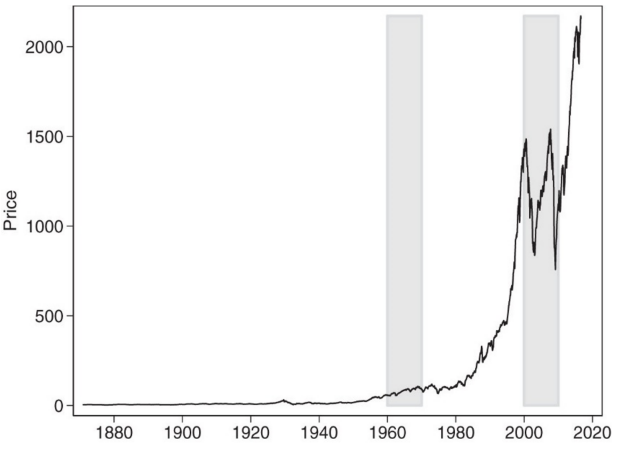
\includegraphics[width=7cm]{pics/sp500 prices.png} }}%
    \qquad
    \subfloat[\centering SP500 Returns over time]{{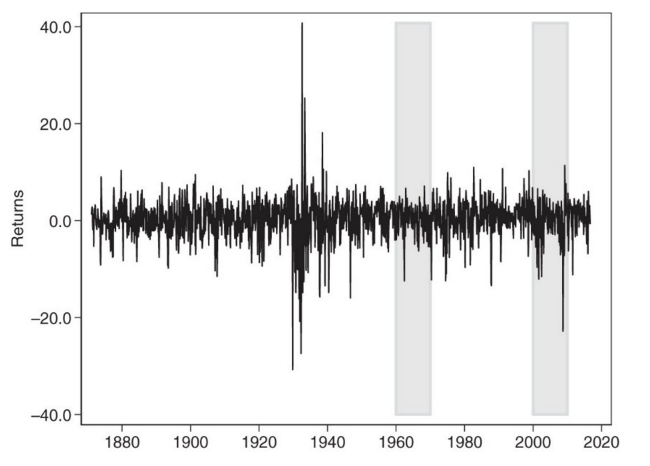
\includegraphics[width=7cm]{pics/sp500 returns.png} }}%
    \caption{Stationary Dynamics of Prices vs Returns}%
    \label{fig:prices vs returns}%
\end{figure}

We can see quite evidently from Figure \ref{fig:prices vs returns} that the price series of the S\&P 500 index is not stationary, while the returns are closer. If we wanted to model the price series we must use cointegration.

\subsection{AutoRegressive Models}
The simplest possible dynamic model is an autoregressive model of order 1 or AR(1) model

\begin{definition}
    AR(1) and AR(p) models:
    \begin{equation}
        \label{AR1 model}
        y_t = \phi_0 + \phi_1 y_{t-1} + u_t, \qquad u_t \sim i.i.d(0,\sigma_u^2).
    \end{equation}
    The condition $|\phi_1|<1$ is required for the model to be stationary.

If the longest lag included is the $p^{th}$ lag, then we have:

\begin{equation}
\label{ARp model}
y_t=\phi_0+\phi_1 y_{t-1}+\phi_2 y_{t-2}+\cdots+\phi_p y_{t-p}+u_t, \quad u_t \sim i i d\left(0, \sigma_u^2\right)
\end{equation}
\end{definition}

\subsubsection{AR(1) Models}

We have the following vector of unknown parameters: $\{\phi_0, \phi_1, \sigma_u^2\}$, which can be estimated by OLS. If we have 
\[y_t = \phi_0 + \phi_1 y_{t-1} + u_t, \qquad u_t \sim i.i.d(0,\sigma_u^2).
    \]
    if we take unconditional expectations of both sides we have:
    \[E(y_t) = E(\phi_0 + \phi_1 y_{t-1} + u_t) = \phi_0 + \phi_1 E(y_{t-1})\]

    Stationarity implies $E(y_t) = E(y_{t-1})$ therefore we can rearrange:
    

    \begin{definition}
    Expected Mean of the AR(1) model:
        \[E(y_t) = \dfrac{\phi_0}{1-\phi_1}.\]
    \end{definition}


Unconditional Variance of AR(1) models:

\[var(y_t) = \gamma_0 = E[(y_t - E(y_t))^2].\]
Recognising that  
\[y_t - E(y_t) = \phi_0 + \phi_1 y_{t-1} + u_t - \phi_0 - \phi_1 E(y_{t-1} = \phi_1 [y_t - E(y_{t-1})] + u_t\]

Squaring both sides and taking unconditional expectations we have:
\begin{align*}
    E\{[y_t-E(y_t)]^2\} &= \phi_1^2 E\{[y_{t-1} - E(y_{t-1})]^2\} + E(u_t^2) + 2 E\{[y_{t-1}-E(y_{t-1})]u_t\} \\
    & = \phi_1^2 E\{[y_{t-1} - E(y_{t-1})]^2\}+ E(u_t^2)
\end{align*}
from $E\{[y_{t-1}-E(y_{t-1})]u_t\} = 0$. Because from before we have:
\[\gamma_0 = E\{[y_t - E(y_t)]^2\} = E\{[y_{t-1} - E(y_{t-1})]^2\}\]

which represents the variance of $y_t$. It follows that:
\[\gamma_0 = \phi_1^2 \gamma_0 + \sigma_u^2,\]
giving us:
\begin{definition}
    Unconditional Variance of AR(1) models:
    \[\gamma_0 = \dfrac{\sigma_u^2}{1-\phi_1^2}\]
\end{definition}

We can solve for our vector of unknown parameters through OLS. Once we have these values we can calculate our disturbance term $\hat{u}_t$:
\begin{equation}
\widehat{u}_t=y_t-\widehat{\phi}_0-\widehat{\phi}_1 y_{t-1}
\end{equation}

\begin{definition}
    Residual Sum of Squares of AR(1) model:
    \begin{equation}
S=\sum_{t=2}^T u_t^2=\sum_{t=2}^T\left(y_t-\phi_0-\phi_1 y_{t-1}\right)^2
\end{equation}
where the sample sum of squares begins at $t=2$ as 1 observation is lost because of the inclusion of 1 lag in the model.
\end{definition}



The variance of the residual is:
\begin{equation}
\widehat{\sigma}_u^2=\frac{1}{T-1} \sum_{t=2}^T \widehat{u}_t^2
\end{equation}

\subsubsection{AR(p) Models}

Now we have more unknown parameters which makes our vector:$ \theta=\left\{\phi_0, \phi_1, \cdots, \phi_p, \sigma_u^2\right\}$.

\begin{definition}
    The Residual Sum of Squares for the AR(p) model is:
    \begin{equation}
S=\sum_{t=p+1}^T u_t^2=\sum_{t=p+1}^T\left(y_t-\phi_0-\phi_1 y_{t-1}-\phi_2 y_{t-2}-\cdots-\phi_p y_{t-p}\right)^2
\end{equation}
where the sample sum of squares begins at $t=p+1$ as $p$ observations are lost because of the inclusion of $p$ lags.
\end{definition}

After estimating the parameters through OLS, the least squares residuals are computed as:
\begin{equation}
\widehat{u}_t=y_t-\widehat{\phi}_0-\widehat{\phi}_1 y_{t-1}-\widehat{\phi}_2 y_{t-2}-\cdots-\widehat{\phi}_p y_{t-p}
\end{equation}
which are used to compute the variance of the residual:
\begin{equation}
\widehat{\sigma}_u^2=\frac{1}{T-p} \sum_{t=p+1}^T \widehat{u}_t^2
\end{equation}

\subsection{Moving Average Models}

An alternative way to model univariate dynamics is the Moving Average (MA) model. 


\begin{definition}
An \textbf{MA(1)} model is defined as :
\begin{equation}
y_t=\psi_0+u_t+\psi_1 u_{t-1}, \quad u_t \sim \operatorname{iid}\left(0, \sigma_u^2\right)
\end{equation}
We use lag dynamics in the disturbance term to model the dynamics in the dependent variable. The condition $|\psi_1|<1$ is required for the model to be stationary.
\end{definition}


\begin{definition}
    An \textbf{MA(q)} is defined as:
    \begin{equation}
y_t=\psi_0+u_t+\psi_1 u_{t-1}+\psi_2 u_{t-2}+\cdots+\psi_q u_{t-q}, \quad u_t \sim \text { iid }\left(0, \sigma_u^2\right)
\end{equation}
The $q^{th}$ lag is the longest lag used yo model the dynamics in the dependent variable, $y_t$.
\end{definition}

Unlike the AR(p), \textit{we do not have} an analytical solution to the MA(q) parameters, because the first order condition is nonlinear with unobserved lagged disturbances.


\subsection{ARMA Models}

We can combine AR and MA models for an \textbf{AutoRegressive Moving Average} (ARMA) model. For example this ARMA(1,1) model:

\begin{equation}
\label{ARMA(1,1)}
y_t=\phi_0+\phi_1 y_{t-1}+u_t+\psi_1 u_{t-1}, \quad u_t \sim \text { i.i.d }\left(0, \sigma_u^2\right)
\end{equation}

This can easily be extended to the ARMA(p,q) model:
\begin{equation}
y_t=\phi_0+\phi_1 y_{t-1}+\cdots+\phi_p y_{t-p}+u_t+\psi_1 u_{t-1}+\cdots+\psi_q u_{t-q} \quad u_t \sim \operatorname{iid}\left(0, \sigma_u^2\right) .
\end{equation}

Because of the MA Component, the ARMA parameters also require numerical optimisation. We assume some initial values of the disturbances and update them as we estimate $\phi$s and $\psi$s.

Our final estimates will be the ones that minimise the objective function after many iterations.
\begin{note}
    This can also be done in two steps. We estimate the disturbances. Conditional on those estimates being almost right we can predict the $\phi$s and $\psi$s.
\end{note}

\subsubsection{Regression models with dynamics}

To allow for dynamic effects, regression models may be combined with the ARMA class of models. This can be done by specifying the disturbance/error terms as AR or MA models.

\begin{align*}
    y_t=\alpha+\beta x_t+u_t, \quad u_t=\phi_1 u_{t-1}+v_t & \text { [AR disturbance] } \\
    y_t=\alpha+\beta x_t+u_{t,} \quad u_t=v_t+\psi_1 v_{t-1} & \text { [MA disturbance] } \\
    y_t=\alpha+\beta x_t+\lambda y_{t-1}+u_t & \text { [Lagged dependent] } \\
    y_t=\alpha+\beta x_t+\gamma x_{t-1}+u_t & \text { [Lagged explanatory] } \\
    y_t=\alpha+\beta x_t+\lambda y_{t-1}+\gamma x_{t-1}+u_t & \text { [Joint specification] } \\
    u_t=\phi_1 u_{t-1}+v_t+\psi_1 v_{t-1} . &
\end{align*}

These are all univariate models. Including these dynamics in a regression model allows us to correct for potential misspecification problems that arise from incorrectly excluding explanatory variables. \textbf{Misspecification (ignoring lags, and leads) leads to inefficiency.}


We can test for misspecification by testing for autocorrelation, heteroskedasticity, and normality in the residuals.

\subsection{(Partial) Autocorrelation Function}
\subsubsection{Autocorrelation Function}

Consider the following sequence of AR models may be estimated equation-by-equation by OLS:
\begin{equation}
\begin{aligned}
& y_t=\phi_{10}+\rho_1 y_{t-1}+u_{1 t} \\
& y_t=\phi_{20}+\rho_2 y_{t-2}+u_{2 t} \text {, } \\
& \vdots \quad \vdots \quad \vdots \\
& y_t=\phi_{k 0}+\rho_k y_{t-k}+u_{k t}, \\
&
\end{aligned}
\end{equation}
which gives us the estimated autocorrelation function (ACF) $\{\hat{\rho}_1, \hat{\rho}_2, \ldots, \hat{\rho}_k\}$. Note that the constant differs between each equation.

With our AR(1) model we had:
\begin{equation}
y_t=\phi_0+\phi_1 y_{t-1}+u_t, \quad u_t \sim i i d\left(0, \sigma_u^2\right)
\end{equation}

For $0<\phi_1<1$, the autocorrelation function of $y_t$ declines exponentially for increasing $k$ so that the effects of previous values on $y_t$ gradually diminish.

For $-1<\phi_1<0$ the autocorrelation coefficient $y_t$ alternates in sign as $k$ is even or odd, \textbf{and its modulus declines exponentially}

\begin{figure}[h]
    \centering
    \subfloat[\centering AR(1) ACF $\phi=0.8$]{{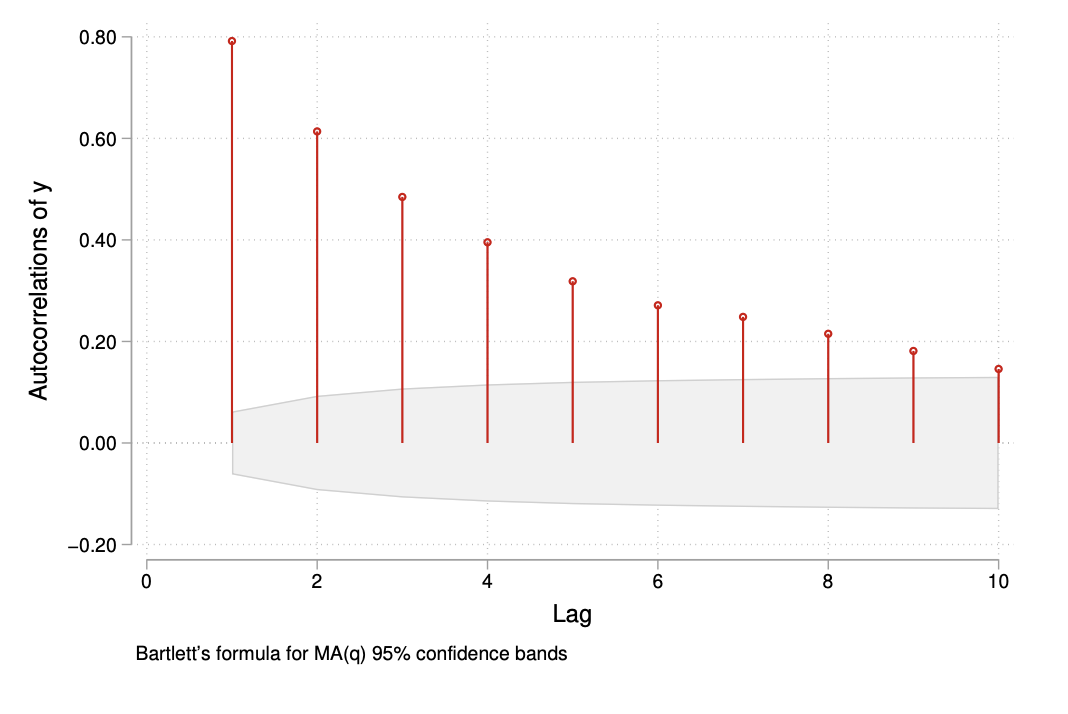
\includegraphics[width=7cm]{pics/positive acf.png} }}%
    \qquad
    \subfloat[\centering AR(1) ACF $\phi=-0.8$]{{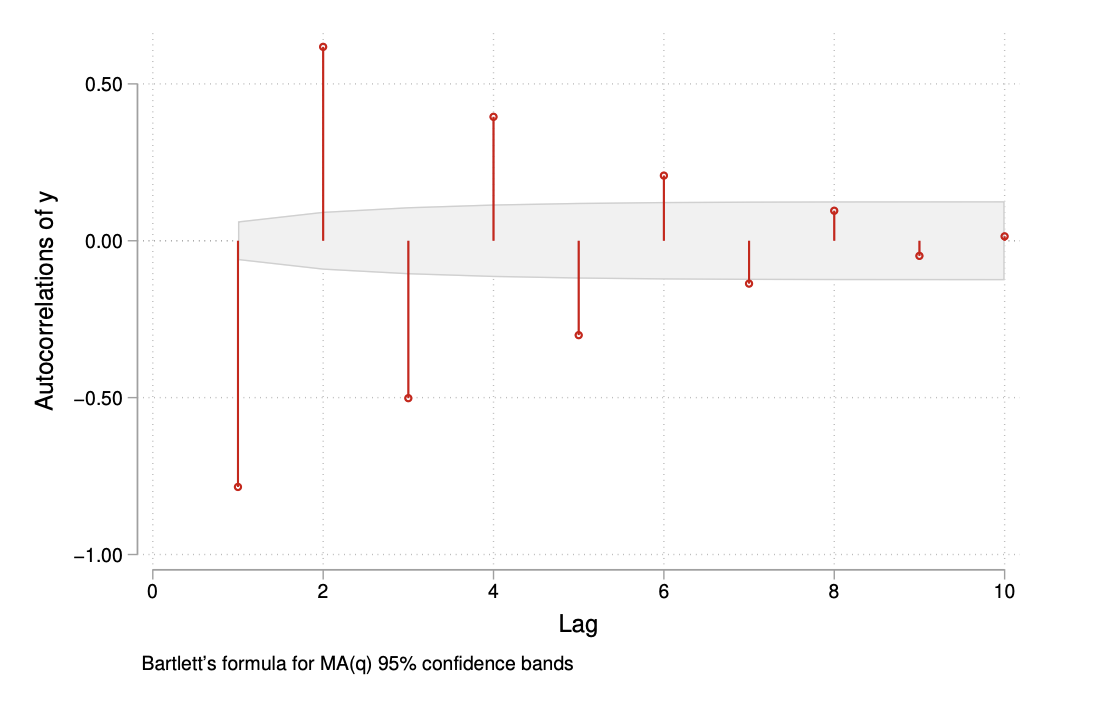
\includegraphics[width=7cm]{pics/negative acf.png} }}%
    \caption{Autocorrelation Function of AR(1) models}%
    \label{fig:positive negative acf}%
\end{figure}


\subsubsection{Partial Autocorrelation Function}

Another measure of the dynamic properties of AR models is the partial autocorrelation function (PACF) at lag $k$. This measures the relationship between $y_t$ and $y_{t-k}$ but now with the intermediate lags included in the regression model so that their effects are controlled for. 

We use OLS to estimate the following AR models:
\begin{equation}
\label{PACF estimation equations}
\begin{aligned}
& y_t=\phi_{10}+\phi_{11} y_{t-1}+u_{1 t} \\
& y_t=\phi_{20}+\phi_{21} y_{t-1}+\phi_{22} y_{t-2}+u_{2 t} \\
& y_t=\phi_{30}+\phi_{31} y_{t-1}+\phi_{32} y_{t-2}+\phi_{33} y_{t-3}+u_{3 t} \\
& \vdots \quad \vdots \quad \vdots \quad \vdots \\
& y_t=\phi_{k 0}+\phi_{k 1} y_{t-1}+\phi_{k 2} y_{t-2}+\cdots+\phi_{k k} y_{t-k}+u_{k t} \\
&
\end{aligned}
\end{equation}

The estimated PACF is given by $\left\{\widehat{\phi}_{11}, \widehat{\phi}_{22}, \cdots, \widehat{\phi}_{k k}\right\}$.

The PACF for an AR(p) model is 0 for lags greater than $p$. For example, in the AR(1) model the PACF has a \textbf{spike at lag 1} and thereafter is $\phi_{kk}=0, \forall k>1$.

This is where the PACF and ACF differ because in general, the ACF has non-zero values for higher lags.

\begin{figure}[h]
    \centering
    \subfloat[\centering AR(1) PACF $\phi=0.8$]{{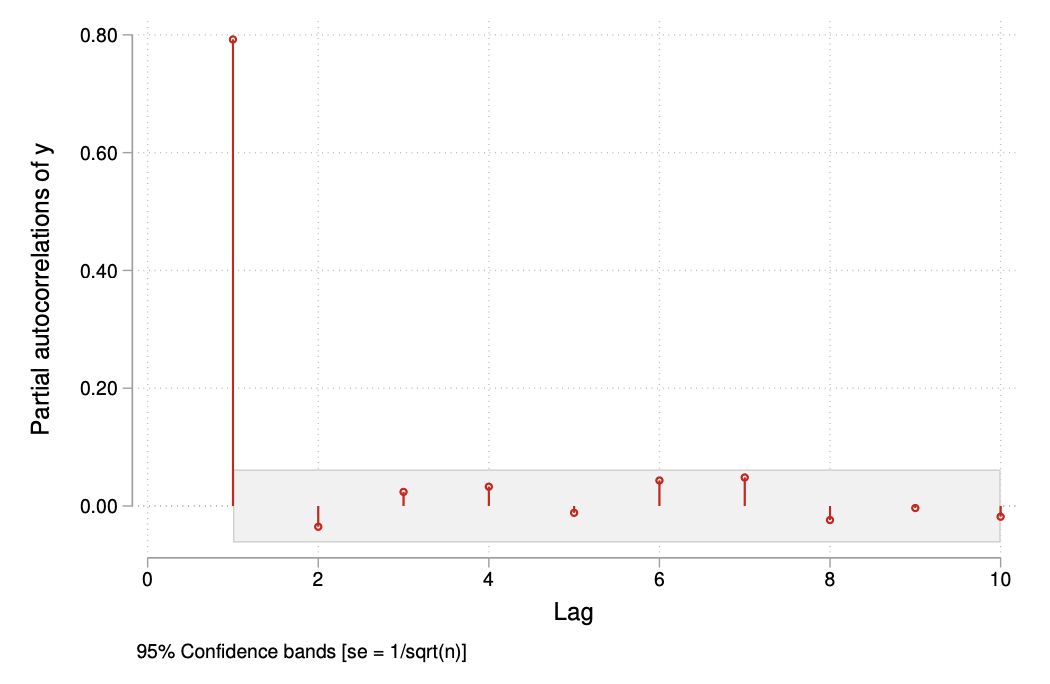
\includegraphics[width=7cm]{pics/positive pacf.png} }}%
    \qquad
    \subfloat[\centering AR(1) PACF $\phi=-0.8$]{{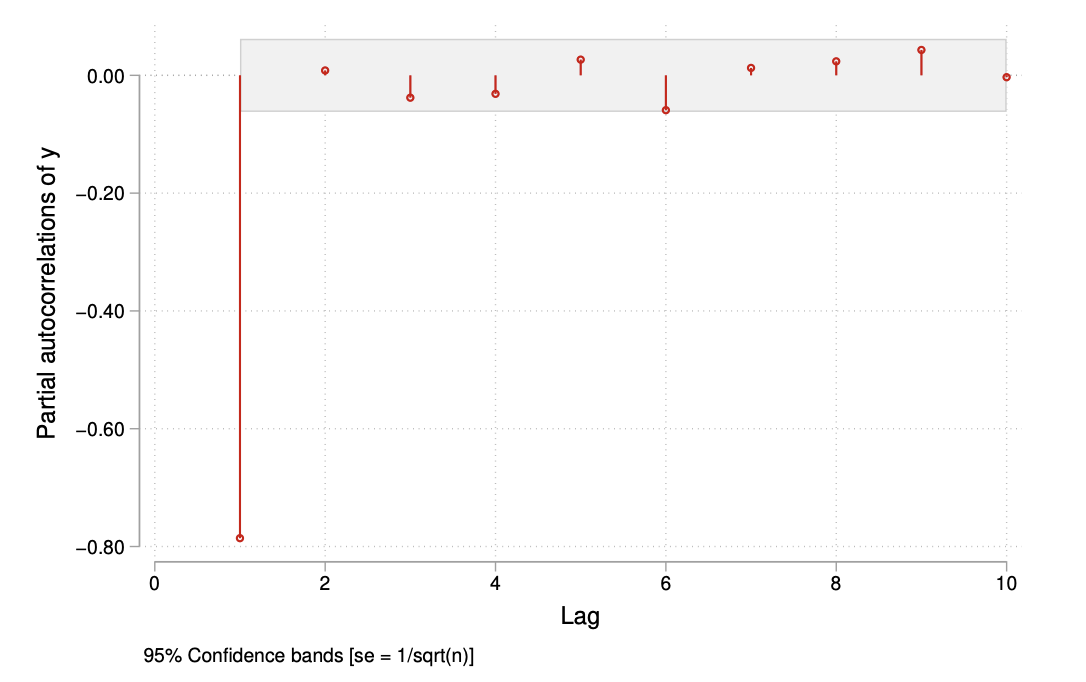
\includegraphics[width=7cm]{pics/negative pacf.png} }}%
    \caption{Partial Autocorrelation Function of AR(1) models}%
    \label{fig:positive negative pacf}%
\end{figure}


\paragraph{ACF and PACF for MA models}
So far we have only looked at the ACF and PACF in the context of an AR model. Now we will look at what we expect in the context of an MA model.

Recall:
\begin{equation}
y_t=\psi_0+u_t+\psi_1 u_{t-1}, \quad u_t \sim \operatorname{iid}\left(0, \sigma_u^2\right)
\end{equation}

\begin{figure}[ht]
    \centering
    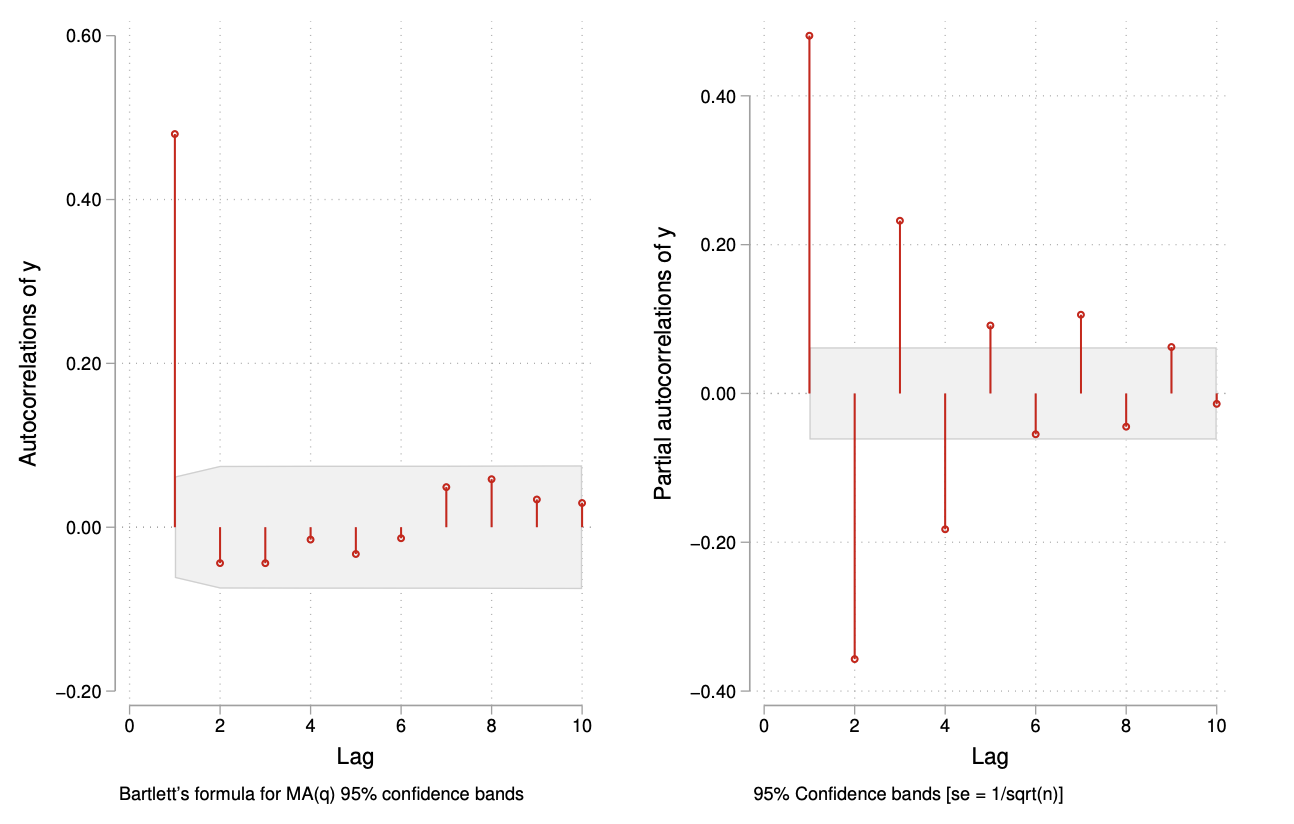
\includegraphics[width=10cm]{pics/ma positive.png}
    \caption{MA(1) with Positive ACF and PACF }
    \label{fig:ma acf pacf positive}
\end{figure}

\begin{note}
    An MA(1) can be re-expressed as an AR($\infty$). We see flipped results with MA compared to AR. The PACF declines exponentially rather than the spike we see in the AR model. The positive $\psi_1$ in the MA model \textbf{oscillates} in the \textbf{PACF}, while the positive $\phi_1$ \textbf{declines exponentially} in the \textbf{ACF}
\end{note}

\begin{figure}[ht]
    \centering
    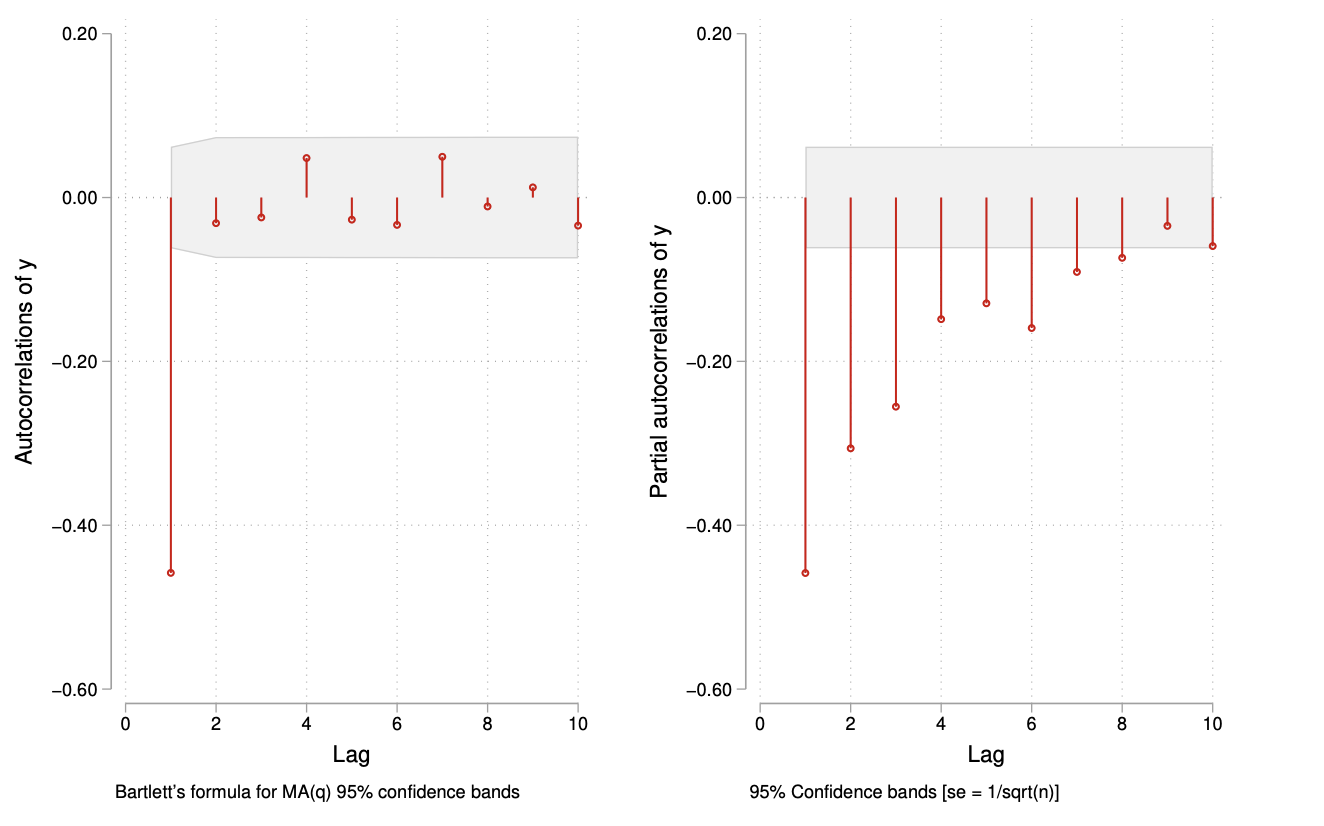
\includegraphics[width=10cm]{pics/ma negative.png}
    \caption{MA(1) with Negative ACF and PACF }
    \label{fig:ma acf pacf negative}
\end{figure}

\begin{table}[ht]
    \centering
    \begin{tabular}{ |c|c|c| } 
    \hline
 & ACF & PACF \\
 \hline
 AR(p) & declines exponentially or oscillates & spike and cuts off \\ 
 \hline
 MA(q) & spike and cuts off & Declines exponentially or oscillates \\ 
 \hline
 ARMA & Declines exponentially of oscillates after $q$ lags & Declines exponentially or oscillates after $p$ lags \\ 
 \hline
\end{tabular}
    \caption{Criteria to find ARMA models.}
    \label{tab:arma table}
\end{table}

\newpage
\clearpage

\subsection{Vector Autoregression Models (VAR)}

Sometimes it is difficult to delimit a single variable as the \textbf{dependent} variable to be explained in terms of all other variables - it is reasonable to suppose that all variables are jointly determined.

In a multiple equation system where each variable is dependent on its own lags and the lags of all other variables, then we have a vector autoregression. We have included the dynamic effects to allow the financial variables to adjust to shocks over time.
\begin{note}
    The assumption of stationarity of all variables is maintained.
\end{note}

\subsubsection{VAR(1) with 2 variables}
An example of a two variable VAR(1) model is:

\begin{equation}
\begin{aligned}
& y_{1 t}=\phi_{10}+\phi_{11,1} y_{1 t-1}+\phi_{12,1} y_{2 t-1}+u_{1 t} \\
& y_{2 t}=\phi_{20}+\phi_{21,1} y_{1 t-1}+\phi_{22,1} y_{2 t-1}+u_{2 t}
\end{aligned}
\end{equation}
where $y_{1t}$ and $y_{2t}$ are the jointly depndent variables and $u_{1t}$ and $u_{2t}$ are disturbance terms.

\begin{note}
Apart from the intercepts, each coefficient has three subscripts.
\begin{itemize}
    \item The first subscript identifies the equation to which the coefficient belongs.
    \item The second subscript identifies the variable to which it is attached.
    \item The third subscript identifies the lag to which it pertains.
\end{itemize}
\end{note}

\subsubsection{Other VAR Specifications}
\begin{note}
    We cannot have ARMA in VAR models because we have no observed $u_{t-1}$.
\end{note}

\paragraph{VAR(2) with 2 Variables}

\begin{equation}
\begin{aligned}
& y_{1 t}=\phi_{10}+\phi_{11,1} y_{1 t-1}+\phi_{11,2} y_{1 t-2}+\phi_{12,1} y_{2 t-1}+\phi_{12,2} y_{2 t-2}+u_{1 t} \\
& y_{2 t}=\phi_{20}+\phi_{21,1} y_{1 t-1}+\phi_{21,2} y_{1 t-2}+\phi_{22,1} y_{2 t-1}+\phi_{22,2} y_{2 t-2}+u_{2 t}
\end{aligned}
\end{equation}

\paragraph{VAR(1) with three variables}

\begin{equation}
\begin{aligned}
& y_{1 t}=\phi_{10}+\phi_{11,1} y_{1 t-1}+\phi_{12,1} y_{2 t-1}+\phi_{13,1} y_{3 t-1}+u_{1 t} \\
& y_{2 t}=\phi_{20}+\phi_{21,1} y_{1 t-1}+\phi_{22,1} y_{2 t-1}+\phi_{23,1} y_{3 t-1}+u_{2 t} \\
& y_{3 t}=\phi_{30}+\phi_{31,1} y_{1 t-1}+\phi_{32,1} y_{2 t-1}+\phi_{33,1} y_{3 t-1}+u_{3 t}
\end{aligned}
\end{equation}
where $y_{1t}, y_{2t}, y_{3t}$ are the jointly dependent variables.

\paragraph{VAR(p) with three variables}
\begin{equation}
\begin{aligned}
& y_{1 t}=\phi_{10}+\sum_{i=1}^p \phi_{11, i} y_{1 t-i}+\sum_{i=1}^p \phi_{12, i} y_{2 t-i}+\sum_{i=1}^p \phi_{13, i} y_{3 t-i}+u_{1 t} \\
& y_{2 t}=\phi_{20}+\sum_{i=1}^p \phi_{21, i} y_{1 t-i}+\sum_{i=1}^p \phi_{22, i} y_{2 t-i}+\sum_{i=1}^p \phi_{23, i} y_{3 t-i}+u_{2 t} \\
& y_{3 t}=\phi_{30}+\sum_{i=1}^p \phi_{31, i} y_{1 t-i}+\sum_{i=1}^p \phi_{32, i} y_{2 t-i}+\sum_{i=1}^p \phi_{33, i} y_{3 t-i}+u_{3 t}
\end{aligned}
\end{equation}
$p$ is a prescribed lag length which is the same for all equations. $u_t$ is \textbf{uncorrelated} across equations with \textbf{OLS}, $u_t$ is \textbf{correlated} across equations with most \textbf{likelihood}.


\subsubsection{Higher Dimensional VAR Models}

In matrix notation a VAR model with $N$ variables is represented as:
\begin{equation}
y_t=\Phi_0+\Phi_1 y_{t-1}+\Phi_2 y_{t-2}+\cdots+\Phi_p y_{t-p}+u_t
\end{equation}

Where the parameter matrices are given by:
\begin{equation}
\Phi_0=\left[\begin{array}{c}
\phi_{10} \\
\phi_{20} \\
\vdots \\
\phi_{N 0}
\end{array}\right], \quad \Phi_i=\left[\begin{array}{cccc}
\phi_{11, i} & \phi_{12, i} & \cdots & \phi_{1 N, i} \\
\phi_{21, i} & \phi_{22, i} & & \phi_{2 N, i} \\
\vdots & \vdots & \ddots & \vdots \\
\phi_{N 1, i} & \phi_{N 2, i} & \cdots & \phi_{N N, i}
\end{array}\right]
\end{equation}

The disturbances $u_t=\left\{u_{1 t}, u_{2 t}, \ldots, u_{N t}\right\}^{\prime} \sim \operatorname{iid}(0, \Omega)$ has zero mean and are represented in the covariance matrix:
\begin{equation}
    \Omega=\mathrm{E}\left(u_t u_t^{\prime}\right)=\left[\begin{array}{llll}\sigma_1^2 & \sigma_{12} & \cdots & \sigma_{1 N} \\ \sigma_{21} & \sigma_2^2 & \cdots & \sigma_{2 N} \\ \vdots & \vdots & \ddots & \vdots \\ \sigma_{N 1} & \sigma_{N 2} & \cdots & \sigma_N^2\end{array}\right]
\end{equation}

\begin{note}
    The $\phi_0$ amtrix contains $N$ parameters, $\phi_1$ matrix has $N^2$ parameters. We have $p \phi_i$ matrices. Therefore the total number of parameters we must estimate is $(Np+1)N$. Adding one lag increases the number of parameters by $N^2$. Adding one more \textit{variable} increases the number of parameters by $2Np + p + 1$. 

    Every time we add a parameter we lose one degree of freedom for estimation
\end{note}

\paragraph{Covariance Matrix of residuals} \mbox{}

To estimate $\Omega$ let $\hat{u}_t = \{\hat{u}_{1t}, \hat{u}_{2t}, \ldots, \hat{u}_{Nt}\}$ represent the least squares residuals for each equation in the VAR. An estimate covariance marix is computed using the sample residuals moment matrix defined by:
\begin{equation}
    \widehat{\Omega}=\left[\begin{array}{cccc}\widehat{\sigma}_1^2 & \widehat{\sigma}_{12} & \cdots & \widehat{\sigma}_{1 N} \\ \widehat{\sigma}_{21} & \widehat{\sigma}_2^2 & & \widehat{\sigma}_{2 N} \\ \vdots & & \ddots & \vdots \\ \widehat{\sigma}_{N 1} & \widehat{\sigma}_{N 2} & \cdots & \widehat{\sigma}_N^2\end{array}\right] =\frac{1}{T}\left[\begin{array}{cccc}\sum_{t=p+1}^T \widehat{u}_{1 t}^2 & \sum_{t=p+1}^T \widehat{u}_{1 t} \widehat{u}_{2 t} & \cdots & \sum_{t=p+1}^T \widehat{u}_{1 t} \widehat{u}_{N t} \\ \sum_{t=p+1}^T \widehat{u}_{2 t} \widehat{u}_{1 t} & \sum_{t=p+1}^T \widehat{u}_{2 t}^2 & & \sum_{t=p+1}^T \widehat{u}_{2 t} \widehat{u}_{N t} \\ \vdots & & \ddots & \vdots \\ \sum_{t=p+1}^T \widehat{u}_{N t} \widehat{u}_{1 t} & \sum_{t=p+1}^T \widehat{u}_{N t} \widehat{u}_{2 t} & \cdots & \sum_{t=p+1}^T \widehat{u}_{N t}^2\end{array}\right]
\end{equation}

\paragraph{Popularity of VAR models} is great in applied research in finance because if a few main reasons:
\begin{enumerate}
    \item Estimation is straightforward. OLS for each equation in the VAR.
    \item The VAR system provides a convenient framework to forecast financial variables
    \item The model provides a basis for performing so-called causality tests between financial variables
    \item Theoretical models in finance can be tested through the imposition of restriction on the VAR parameters.
    \item The dynamics of the VAR can be modelled using impulse response analysis, which reveals the effects of shocks on the system variables.
    \item The volatility of financial variables can be decomposed in terms of their risk components.
    \item There is a convenient link between VAR and Error Correction Models.
\end{enumerate}

\subsubsection{Lag Length Selection}

If the lag length is \textbf{too short}, we risk that aspects of the dynamic mechanism are excluded from the model. If the lag length is \textbf{too long} then there are redundant lags which can reduce the precision of the parameter estimates.

A common \textbf{data-driven} approach to selecting lag order (lag length) is to use \textit{Information Criteria} (IC). The three most commonly used IC are:

\begin{equation}
\begin{aligned}
& A I C=\log |\widehat{\Omega}|+\frac{2 p K^2}{T} \\
& H I C=\log |\widehat{\Omega}|+\frac{2 \log (\log (T))}{T} p K^2 \\
& S I C=\log |\widehat{\Omega}|+\frac{\log (T)}{T} p K^2 .
\end{aligned}
\end{equation}
The SIC is consistent, but less efficient than the other ICs.

\begin{note}
    $\hat{\Omega}$ is the estimation of the covariance matrix, and $K$ is the number of variables. In the scalar case, the determinant of the estimated covariance matrix, $|\hat{\Omega}|$, is replaced by the estimated residual variance, $\hat{\sigma}_u^2$.
\end{note}

\begin{procedure}
    Choosing an IC optimal lag order using any of the above criteria requires the following steps.
    \begin{enumerate}
        \item CHoosing a maximum number of lags, $p_{max}$, for the VAR model. This choice can be informed by the \textit{ACFs and PACFs} of the data, the \textit{frequency} of the observations and the \textit{sample size}.
        \item Estimate the model sequentially for all lags up to and including $p_{max}$. OFr each regression, compute the relevant information criterion, \textbf{holding the sample size fixed}.
        \item We choose the specification based on the \textbf{minimum} values of the IC. 
    \end{enumerate}
    \begin{note}
        In many cases, there will be disagreement between different ICs. The final decision is then a matter of individual judgement.
    \end{note}
\end{procedure}

\subsubsection{VAR Analysis}

In a VAR model, all lagged variables are assumed to contribute information in determining the behaviour of each dependent variable. But we often see large numbers of estimated coefficients that are statistically insignificant. We are less interested in testing all coefficients one by one.


\paragraph{Granger Causality} \mbox{}

We need to know whether \textit{coefficients of all lagged values of a particular explanatory variable in a given equation are \textbf{jointly} zero or not.}

This notion has a close connection with that of causal inference in the sense that \textit{predictions} might be improved by measuring and including such influences.

With our three variable VAR(1) model we have:
\begin{equation}
\begin{aligned}
& y_{1 t}=\phi_{10}+\phi_{11,1} y_{1 t-1}+\phi_{12,1} y_{2 t-1}+\phi_{13,1} y_{3 t-1}+u_{1 t} \\
& y_{2 t}=\phi_{20}+\phi_{21,1} y_{1 t-1}+\phi_{22,1} y_{2 t-1}+\phi_{23,1} y_{3 t-1}+u_{2 t} \\
& y_{3 t}=\phi_{30}+\phi_{31,1} y_{1 t-1}+\phi_{32,1} y_{2 t-1}+\phi_{33,1} y_{3 t-1}+u_{3 t}
\end{aligned}
\end{equation}

The information content of variable $y_2$ on variable $y_1$ might be tested by considering restriction:
\[\phi_{12,1} = 0\]

This restriction can be tested jointly using a $\chi^2$ test with 1 degree of freedom. If $y_{2t}$ plays a role in predicting future values of $y_{1t}$, then $y_{2t}$ is said to cause $y_{1t}$ \textbf{in Granger's sense}.

\begin{note}
    Granger causality is based on the presence or absence of \textbf{predictability} and does not itself signify causal influence. Evidence of Granger causality and the lack of Granger Causality from $y_{2t}$ to $y_{1t}$ are denoted respectively as:
    \begin{equation}
y_{2 t} \rightarrow y_{1 t} \quad y_{2 t} \nrightarrow y_{1 t} .
\end{equation}
\end{note}

We can do these Granger causality test both ways, which can tell us the direction of causality, if it is bidirectional, unidirectional or if the variables are independent.
\begin{equation}
\begin{array}{ll}
\text { Unidirectional: } & y_{1 t} \rightarrow y_{2 t} \\
\text { (from } y_{1 t} \text { to } y_{2 t} \text { ) } & y_{2 t} \nrightarrow y_{1 t} \\
\\
\text { Unidirectional: } & y_{2 t} \rightarrow y_{1 t} \\
\text { (from } y_{2 t} \text { to } y_{1 t} \text { ) } & y_{1 t} \nrightarrow y_{2 t} \\
\\
\text { Bidirectional: } & y_{2 t} \rightarrow y_{1 t} \\
\text { (feedback) } & y_{1 t} \rightarrow y_{2 t} \\
\\
\text { Independence: } & y_{2 t} \nrightarrow y_{1 t} \\
& y_{1 t} \nrightarrow y_{2 t}
\end{array}
\end{equation}

\paragraph{Impulse Response Analysis} \mbox{}

An alternative to Granger Causality tests of identifying the system dynamics of a VAR is \textbf{impulse response}. We do this by tracking the transmission effects of shocks to the system on the dependent variable.

A candidate for the shocks in a VAR system is the vector of disturbances $u_t = \{u_{1t}, u_{2t}, \ldots, u_{Nt}\}$, which represents \textit{contributions to the dependent variable that are not predicted from past information}.

The main \textbf{problem} in the direct use of the fitted disturbances in studying impulse response is that these terms are correlated. This complicates the interpretation of the shocks $u_t$ with respect to the underlying economic and financial forces.

One \textbf{solution} that aids interpretation is to transform the VAR into a new system in which the disturbances in the equations are uncorrelated so that the effects of these uncorrelated shocks on the system variables can be traced over time. \hl{This enables determination of the responses to impulses associated with the individual shocks}.

\paragraph{Illustration of Impulse Response Analysis} \mbox{}

Consider the bivariate VAR(6) model:
\begin{equation}
\label{Impulse illustration original}
\begin{aligned}
& r e_t=\phi_{10}+\sum_{i=1}^6 \phi_{11, i} r e_{t-i}+\sum_{i=1}^6 \phi_{12, i} r d_{t-i}+u_{1 t} \\
& r d_t=\phi_{20}+\sum_{i=1}^6 \phi_{21, i} r e_{t-i}+\sum_{i=1}^6 \phi_{22, i} r d_{t-i}+u_{2 t}
\end{aligned}
\end{equation}
and let the the relationship between the two VAR disturbances $u_{1t}, u_{2t}$, be represented by the linear regression equation:
\[u_{2t} = \rho u_{1t} + v_{2t}\]
where $\rho$ is a parameter capturing the correlation between $u_{2t}$ and $u_{1t}$.

\begin{note}
    $v_{2t}$ is a new disturbance term which, from the properties of the linear regression model, is uncorrelated with $u_{1t}$. 
\end{note}

This equation is a \textbf{structural relationship} between the two shocks, in which the residual is that part of the impulse $u_{2t}$ which is uncorrelated with $u_{1t}$. By replacing $u_{2t}$ in the second equation of \eqref{Impulse illustration original} with $\rho u_{1t} + v_{2t}$ AND by substituting for $u_{1t}$ using the first equation in \eqref{Impulse illustration original} we have:
\begin{equation}
\begin{aligned}
r d_t & =\left(\phi_{20}-\rho \phi_{10}\right)+\rho r e_t+\sum_{i=1}^6\left(\phi_{21, i}-\rho \phi_{11, i}\right) r e_{t-i}+\sum_{i=1}^6\left(\phi_{22, i}-\rho \phi_{12, i}\right) r d_{t-i}+v_{2 t}, \\
& =\beta_{20}+\rho r e_t+\sum_{i=1}^6 \beta_{21, i} r e_{t-i}+\sum_{i=1}^6 \beta_{22, i} r d_{t-i}+v_{2 t},
\end{aligned}
\end{equation}
in which: $\beta_{20}=\phi_{20}-\rho \phi_{10}, \beta_{21, i}=\phi_{21, i}-\rho \phi_{11, i}$ and $\beta_{22, i}=\phi_{22, i}-\rho \phi_{12, i}$.

The difference between the original VAR equation for $rd_t$ in Equation \eqref{Impulse illustration original} and this one is the inclusion of equity returns at time $t$, $re_t$ as an explanatory variable. Also, because $v_{2t}$ is independent of $u_{1t}$, the VAR equation for $re_t$ and this equation for $rd_t$ contain disturbances that are now \textbf{uncorrelated} with each other. The VAR us now called a \textbf{structural VAR (SVAR)}.
\begin{equation}
\label{SVAR re rd}
\begin{aligned}
r e_t & =\beta_{10}+\sum_{i=1}^6 \beta_{11, i} r e_{t-i}+\sum_{i=1}^6 \beta_{12, i} r d_{t-i}+v_{1 t}, \\ 
r d_t & =\beta_{20}+\rho r e_t+\sum_{i=1}^6 \beta_{21, i} r e_{t-i}+\sum_{i=1}^6 \beta_{22, i} r d_{t-i}+v_{2 t},
\end{aligned}
\end{equation}

where $\beta_{10} = \phi_{10}, \beta_{11,i} = \phi_{11,i}, \beta_{12,i} = \phi_{12,i}, v_{1t} = u_{1t}$.

\newpage

\paragraph{Shock to Equity returns} \mbox{}

The estimates of this bivariate SVAR(6) model are:
\begin{table}[h]
    \centering
        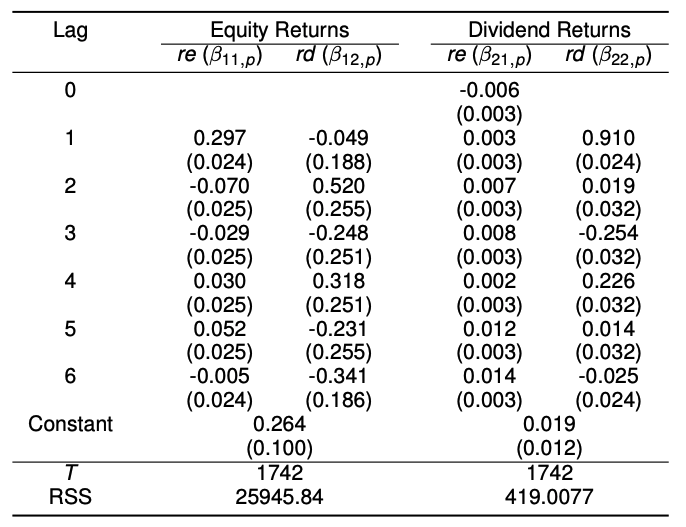
\includegraphics[width=10cm]{pics/impulse response parameter estimates.png}
    \caption{Parameter Estimates for bivariate SVAR(6) model for the United States monthly equity and dividend returns for the period January 1871 to September 2016}
    \label{tab:impulse response analysis parameter estimation}
\end{table}


Impulse responses show the time-forms of system variable responses to incoming structural shocks. To estimate the contemporaneous effect of a shock in $re_t$ on itself, let the size of the shock be equal to the estimate of the standard deviation of $v_{1t}$ which from Table \ref{tab:impulse response analysis parameter estimation} is:

\[\Delta r e_t=\sqrt{\frac{25945.84}{1742}}=3.8593\]

Because the change in $re_t$ is 3.8593, this implies from the SVAR equation for $rd_t$ that dividend returns change by:
\begin{equation}
\Delta r d_t=\widehat{\rho} \times 3.8593=-0.0061 \times 3.8593=-0.0237
\end{equation}

To compute the effect of the equity shock on equities and dividends one period ahead, we rewrite the SVAR in \eqref{SVAR re rd} as:

\begin{equation}
\label{SVAR one period ahead}
\begin{aligned}
& r e_{t+1}=\beta_{10}+\sum_{i=1}^6 \beta_{11, i} r e_{t+1-i}+\sum_{i=1}^6 \beta_{12, i} r d_{t+1-i}+v_{1 t+1} \\
& r d_{t+1}=\beta_{20}+\rho r e_{t+1}+\sum_{i=1}^6 \beta_{21, i} r e_{t+1-i}+\sum_{i=1}^6 \beta_{22, i} r d_{t+1-i}+v_{2 t+1}
\end{aligned}
\end{equation}

Subtracting the SVAR at time $t$ from the SVAR at time $t+1$, we can derive the expected change in equities at time $t+1$:
\begin{equation}
\mathrm{E}_t\left(\Delta r e_{t+1}\right)=\beta_{11,1} \Delta r e_t+\beta_{12,1} \Delta r d_t.
\end{equation}

Therefore, the impulse response of equities at time $t+1$ to an equity shock is estimated as:

\begin{equation}
\mathrm{E}_t\left(\Delta r e_{t+1}\right)=0.2974 \times 3.8593-0.0489 \times(-0.0237)=1.1491
\end{equation}
\begin{note}
    We have used the $\Delta rd_t$ resulting from a 1 s.d. change in $re_t$
\end{note}
\begin{mdframed}
    Check with Yuejun about the change in $re_t$ or $\Delta re_t$
\end{mdframed}

We also know that the expected change in dividends at $t+1$ comes from:
\begin{equation}
\mathrm{E}_t\left(\Delta r d_{t+1}\right)=\rho \Delta r e_{t+1}+\beta_{21,1} \Delta r e_t+\beta_{22,1} \Delta r d_t
\end{equation}
which is estimated as:
\begin{equation}
\mathrm{E}_t\left(\Delta r d_{t+1}\right)=-0.0061 \times 1.1491+0.0028 \times 3.8593+0.9096 \times(-0.0237)=-0.0179 .
\end{equation}

\paragraph{Shock to Dividends} \mbox{}

In the same fashion as before, we let the size of the shock be one standard deviation of $v_{2t}$ which is:

\begin{equation}
\Delta r d_t=\sqrt{\frac{419.0077}{1742}}=0.4904
\end{equation}

The effect of a dividend shock on equities at time $t$ is simply
\[\Delta re_t = 0\]

This is because equity returns are not impacted by contemporaneous shocks to dividends. Only dividends are affected by contemporaneous shocks to equity returns.

The effects of the dividend shock at time $t$ is:

\begin{equation}
\mathrm{E}_t\left(\Delta r e_{t+1}\right)=\beta_{11,1} \Delta r e_t+\beta_{12,1} \Delta r d_t,
\end{equation}

Which is estimated as:
\begin{equation}
\mathrm{E}_t\left(\Delta r e_{t+1}\right)=0.2974 \times 0.00+(-0.0489) \times 0.4904=-0.0240 .
\end{equation}

The effect of a dividend shock on itself next period is:
\begin{equation}
\mathrm{E}_t\left(\Delta r d_{t+1}\right)=\rho \Delta r e_{t+1}+\beta_{21,1} \Delta r e_t+\beta_{22,1} \Delta r d_t
\end{equation}
which is estimated as:
\begin{equation}
\mathrm{E}_t\left(\Delta r d_{t+1}\right)=-0.0061 \times(-0.0241)+0.0028 \times 0.00+0.9097 \times 0.4904=0.4463
\end{equation}

After recursive substitution, STATA calculates the following impulses

\begin{figure}[h]
    \centering
    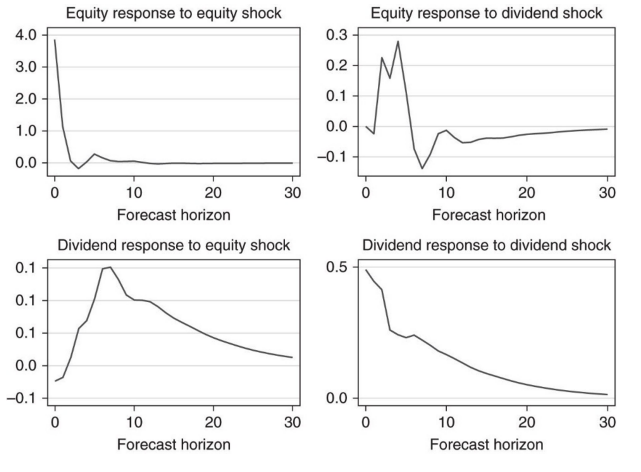
\includegraphics[width=10cm]{pics/impulse response figures.png}
    \caption{Impulse responses for the VAR(6) model of equity and dividend returns. The shaded areas represent 95\% confidence intervals. Data are monthly for the period February 1871 to
September 2016.}
    \label{fig:impulse response analysis figures}
\end{figure}

\subsubsection{Variance Decomposition}

So far we have seen the unscaled absolute impact of various structural shocks. What about the \textbf{relative importance of these shocks}. We can decompose the forecast variance into relative effects, expressed as percentages of the overall movement.

In our SVAR model of equities and dividends, the approach is to express the forecast error variances of equities and dividends in terms of the \textbf{strucutral shocks} $v_1,v_2$.

\paragraph{Forecast Error Variance at T+1} \mbox{}

The forecast error variance of \textbf{equities} at $T+1$ is defined as:

\begin{equation}
\operatorname{var}\left(e_{1 T+1}\right)=\mathrm{E}_T\left[\left(e_{1 T+1}-\mathrm{E}_T\left(e_{1 T+1}\right)\right)^2\right]=\mathrm{E}_T\left(e_{1 T+1}^2\right)=\mathrm{E}_T\left(v_{1 T+1}^2\right)
\end{equation}
which uses the property that $\mathrm{E}_T\left(e_{1 T+1}\right)=0$ and uses the fact that the one-step-ahead forecast error for equities simply equals the equity structural shock
\[e_{1T+1} = v_{1T+1}\]
from the first equation in \eqref{SVAR re rd}. 

This result shows that the equities forecast error variance at $T+1$ is totally determined by its own shocks. This result immediately follows from the \textbf{triangular ordering} of the SVAR model. The forecast error variance of equities at $T+1$ is estimated as

\begin{equation}
\widehat{\operatorname{var}}\left(e_{1 T+1}\right)=3.8593^2=14.8940
\end{equation}
and 100\% of this forecast error variance is the result of own shocks to equities and nothing comes from dividend shocks.

The forecast error variance for \textbf{dividends} can be found by manipulating the second equation in \eqref{SVAR re rd} to show that:
\begin{equation}
e_{2 T+1}=\rho\left(r e_{T+1}-E_T\left(r e_{T+1}\right)\right)+v_{2 T+1}=\rho v_{1 T+1}+v_{2 T+1} .
\end{equation}
Therefore, the forecast error variance of dividends at $T+1$ is:
\begin{equation}
\begin{aligned}
\operatorname{var}\left(e_{2 T+1}\right) & =\mathrm{E}_T\left[\left(\rho v_{1 T+1}+v_{2 T+1}\right)^2\right] \\
& =\mathrm{E}_T\left(\rho^2 v_{1 T+1}^2+v_{2 T+1}^2+2 \rho v_{1 T+1} v_{2 T+1}\right) \\
& =\rho^2 \mathrm{E}_T\left(v_{1 T+1}^2\right)+\mathrm{E}_T\left(v_{2 T+1}^2\right) .
\end{aligned}
\end{equation}

This is estimated as:
\begin{equation}
\widehat{\operatorname{var}}\left(e_{2 T+1}\right)=(-0.0061)^2 \times 3.8593^2+0.49044^2=0.0010+0.24053=0.2411
\end{equation}

This expression shows that for the dividends forecast error variance of 0.2411, $0.49044^2/0.2411 = 0.99766$ or 99.766\% is due to own shocks and the remaining is due to equity shocks.

\begin{table}[h]
    \centering
    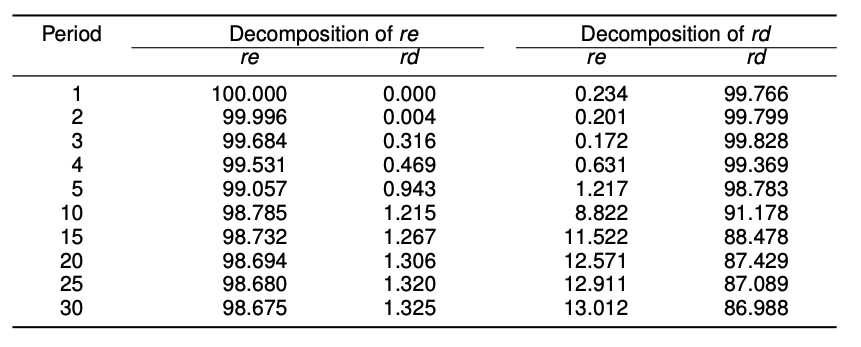
\includegraphics[width=10cm]{pics/variance decomp table.png}
    \caption{Variance decomposition of Equity Returns and Dividends}
    \label{tab:variance decomposition}
\end{table}

An equity shock this period will contribute to 98.675\% of the equity forecast error variance 30 periods (months) later.

\paragraph{Triangular Ordering} \mbox{}

The impulse responses and variance decomposition depend on the ordering of the variables in the VAR. Contemporaneous equity returns enter the equation for dividend returns, but not vice versa. In our example, it makes sense that equity returns impact dividends, and so we arranged the SVAR such that $re_t$ is the first equation and $rd_t$ is the second.

When economic theory and/or common sense strongly suggest that a particular ordering of the variables is appropriate, impulse response analysis and variance decomposition are useful. But often, the choice of ordering in a VAR is arbitrary,







\newpage
\section{Cointegration}
\textbf{Chapter 6}

\subsection{Introduction to Cointegration}
We often see asset prices exhibit strong evidence of trends over long periods of time. Trend behaviours often manifest in a tendency for a time series to drift over time in such a way that no fixed mean value is revealed, i.e. \textbf{price series are nonstationary}.

Consider the equation:
\[y_t = \alpha x_t + v_t\]
There are many different implications to the dependent and/or explanatory variable being non-stationary.

\begin{equation}
\begin{array}{lll}
\hline y_t & x_t & \text { Implications } \\
\hline \text { TS } & \mathrm{I}(0) & \hat{v}_t \text{ will have a time trend}\\
\mathrm{I}(1) & \mathrm{I}(0) & \hat{v}_t \text{ will have a unit root (worse than first case)}\\
\mathrm{I}(0) & \mathrm{I}(1) & \alpha \text{ will be forced to 0}\\
\mathrm{I}(0) & \text { TS } & \alpha \text { will be forced to 0,} x_t \text{ does not contribute to explaining } y_t\\
\text { TS } & \mathrm{I}(1) &  \hat{v}_t\text { will often have a time trend}\\
\mathrm{I}(1) & \text { TS } & \hat{v}_t \text{ will have a unit root} \\
\hline
\end{array}
\end{equation}



In the case where $y_t$ is \textit{trend stationary} and $x_t$ is I(1), if the I(1) process is a unit root with a drift, we will often see no time trend, however when $x_t$ just follows a random walk, we will probably see a time trend.

Inference based on $t, F, \chi^2$ distributions will often be invalid for any of these cases. Obviously, regressions of an I(0) on another I(0) are okay, but there are some cases when we can regress an I(1) on another I(1). This can be done provided the two series are \textbf{cointegrated}.

An important implication of the discussion of stochastic trends and unit roots is that a nonstationary time series can be rendered stationary by differencing. Alternatively, one can achieve stationarity by forming linear combinations of nonstationary series to generate a stationary series.

\begin{definition}
    \textbf{Cointegration}: The ability to generate stationary time series as a linear combination of nonstationary time series. The weights applied to each of the series in the combination are known as the \textbf{cointegrating parameters}.
\end{definition}

\paragraph{Importance of Cointegration} \mbox{}

The existence of cointegration between nonstationar time series has important theoretical, statistical and dynamic implications:
\begin{enumerate}
    \item A number of theoretical models in finance can be expressed by a cointegrating framework
    \item Estimates of the parameters in the cointegrating equations converge to their population vales \textbf{at a faster rate} than in the case for stationary variables, a property known as \textbf{super-consistency}.
    \item Modelling a system of cointegrated variables allows for the joint specification of long-run and short-run dynamics of financial variables in terms of the VECM
\end{enumerate}


\subsection{Present Value Model}

\begin{figure}[h]
    \centering
    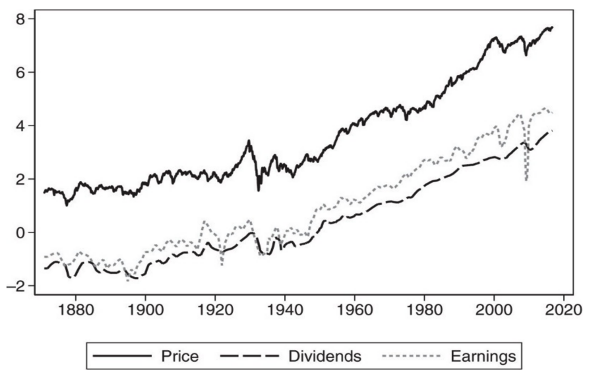
\includegraphics[width=10cm]{pics/us equity prices.png}
    \caption{Time Series Plot of monthly US log equity prices, log dividend payments and log earnings per share from Jan 1871 to Sep 2016.}
    \label{fig:us equity prices}
\end{figure}
Even though the equity prices and dividends are potentially I(1), the present value model of equity prices suggests a theoretical relationship between them. This is expressed as:

\begin{equation}
    \label{present value model og}
    p_t = \beta_0 + \beta_d d_t + u_t,
\end{equation}

where $p_t$ is log equity price, $d_t$ is the log dividend, $u_t$ is a disturbance term and $\beta_0,\beta_1$ are unknown parameters.

Both $p_t$ and $d_t$ are well-modelled as I(1) processes, yet the present value model indicates that the differences $p_t - \beta_0 - \beta_d d_t = u_t$ are simply transient shocks that do not disturb the nature of the relationship over time. Because of this the relationship between $p_t$ and $d_t$ in Equation \eqref{present value model og} is therefore regarded as a long-run or permanent relationship between trending I(1) series and the disturbances $u_t$ are viewed as transient shocks of I(0).

The linear combination of the I(1) variables $p_t$ and $d_t$ that results in the I(0) variable given by $u_t$ is known as a cointegrating relationship. In this model, both $\beta_0$ and $\beta_d$ are cointegrating parameters. $\beta_0$ is the average spread (price-dividends), and obviously $\beta_d$ is the partial effect of dividends on equity prices.

Another way to see the present value model as a cointegrating system is through a scatter diagram.
\begin{figure}[h]
    \centering
    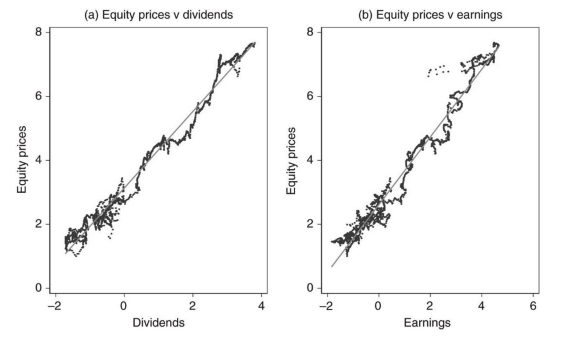
\includegraphics[width=10cm]{pics/price dividends scatter.png}
    \caption{Scatter plots of monthly US log equity prices and log dividends}
    \label{fig:equity dividends scatter}
\end{figure}

The line we see in this plot is
\[p_t = 3.1375 + 1.1957 d_t + \hat{u}_t.\]

Even though $p_t$ and $d_t$ are both I(1) processes, prices and dividends never deviate too far from the line, suggesting that this is a dynamic equilibrium line.
\begin{note}
    If there was no cointegration the scatter diagram would have points evenly scattered over 2-dimensions. In other words, cointegration has the effect of compressing equity prices and dividends from 2 dimensions to 1.
\end{note}

\subsubsection{Equilibrium Adjustment}

This interpretation of the scatter diagram also suggests that actual movement in $p_t$ can be decomposed into a long-run component representing the dynamic equilibrium price as determined by dividends, and a short-run component representing the temporary deviations of $p_t$ from its long-run. This decomposition is expressed as:

\begin{equation}
\underbrace{p_t}_{\text {Actual }}=\underbrace{\beta_0+\beta_d d_t}_{\text {Long-run }}+\underbrace{u_t}_{\text {Short-run }}
\end{equation}

To understand the equilibrating mechanisms of the present value model consider the effects of a shock at time $t$, as given by $u_t$, assuming that dividends are not affected initially.
\begin{enumerate}
    \item Positive shock, $u_t>0$: equities are over values relative to the long-run level with the stock price operating above its long-run equilibrium
    \item Negative shock, $u_t<0$: equities are undervalued with $p_t$ operating below the long-run price.
\end{enumerate}

An equilibrium relationship implies that any shock to the system will result in an adjustment taking place in such a way that equilibrium is eventually restored.

\subsubsection{Equilibrium Dynamics}

\begin{figure}[h]
    \centering
    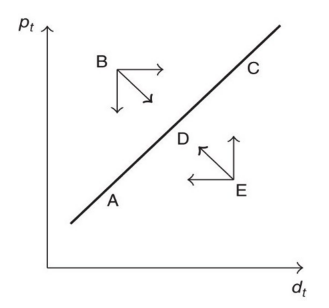
\includegraphics[width=12cm]{pics/equilibrium adjustment.png}
    \caption{Phase diagram to demonstrate the equilibrium adjustment if two variables are cointegrated}
    \label{fig:equilibrium adjustment}
\end{figure}

The line of ADC represents the equilibrium line of the present value model, and pressure from points B and E above and below the line drive the system towards the equilibrium path. Consider a shock at time $t$, assuming initially dividends, $d_t$, are unaffected. For a positive shock equities appear overvalued relative to the long-run level since the stock price lies above its long-run equilibrium price as determined by dividend flows (point B). A negative shock implies equities are undervalued because $p_t$ lies below its long0run equilibrium price (point E).

\paragraph{Potential Shocks} \mbox{}

\begin{enumerate}
    \item Equity price adjust:
    For equilibrium to be re-established in this scenario, equity prices need to decrease back to point A from B without any change in dividends. Assuming that the fall in equity prices is proportional to the size of the shock $u_t = p_t - \beta_0 -\beta_d d_t$, the change in the equity price in the next period $p_{t+1}-p_t$ is represented by the \textbf{adjustment equation}:
    \begin{equation}
\Delta p_{t+1}=p_{t+1}-p_t=\delta_1+\alpha_1\left(p_t-\beta_0-\beta_d d_t\right)+v_{1 t+1}
\end{equation}
Equity prices adjust downward, B to A keeping $d_t$ constant (B to A|$d_t$), or upward (E to C$|d_t$) to restore equilibrium.
\begin{note}
    $\alpha_1<0$
\end{note}
\item Dividends adjust:
Here we assuming prices remain constant, and thus a positive shock implying the price is above the long-run equilibrium price (B), dividends must adjust \textbf{upward} (B to C|$p_t$). Or a negative shock means dividends must adjust downward (E to A|$p_t$).
\begin{note}
    $\alpha_1>0$
\end{note}
\item Equity and Dividends Adjust:
When $p_t$ and $d_t$ both deviate, the relative strength of the movement in equity prices and dividends is determined by the magnitudes of $\alpha_1$ and $\alpha_2$. In our graph, if there is a movement from B to D, then this means that both equity and dividends bear an equal share of the adjustment toward equilibrium.
\end{enumerate}

\begin{example}
    Present Value Model in the US

    To gauge the relative strength of the adjustment parapmeters $\alpha_1, \alpha_2$ in restoring equilibrium in the PV model for the US, we just estimate the price and dividend adjustment equations with OLS.

    $\hat{u}_{t+1}$ represents the OLS residuals from the cointegrating regression, 
    \begin{equation}
\begin{aligned}
\Delta p_t & =0.0035-0.0011 \widehat{u}_{t-1}+\widehat{v}_{1 t} \\
\Delta d_t & =0.0029+0.0078 \widehat{u}_{t-1}+\widehat{v}_{2 t}
\end{aligned}
\end{equation}
We see that the signs are consistent with the dynamics, and because:
\begin{equation}
\left|\widehat{\alpha}_2\right|=0.0078>\left|\widehat{\alpha}_1\right|=0.0011
\end{equation}
dividends are the main driving force in restoring equilibrium in the system after a shock to the equity price.
\end{example}

\subsection{Error Correction Models}

Consider the system:
\begin{equation}
\begin{aligned}
& \Delta p_t=\delta_1+\alpha_1\left(p_{t-1}-\beta_0-\beta_d d_{t-1}\right)+v_{1 t} \\
& \Delta d_t=\delta_2+\alpha_2\left(p_{t-1}-\beta_0-\beta_d d_{t-1}\right)+v_{2 t} .
\end{aligned}
\end{equation}
We may want to include lags of $\Delta p_t$ and $\Delta d_t$ if $v_{1t}, v_{2t}$ are autocorrelated. The long-run relationship
\[u_{t-1} = p_{t-1} - \beta_0 - \beta_d d_{t-1}\]
is common to both equations. We can therefore rewrite the system as:
\begin{equation}
\begin{aligned}
& \Delta p_t=\delta_1+\alpha_1\left(u_{t-1}\right)+v_{1 t} \\
& \Delta d_t=\delta_2+\alpha_2\left(u_{t-1}\right)+v_{2 t}
\end{aligned}
\end{equation}
This form is known as the \textbf{Error Correction Model} because the system behaves in such a way as to correct the equilibrium errors, $u_{t-1}$.

\subsubsection{Vector Error Correction Models}

In general, the simplest bivariate vector error correction model (VECM) is given by:
\begin{equation}
\begin{aligned}
& \Delta y_{1 t}=\delta_1+\alpha_1\left(y_{1 t-1}-\beta_0-\beta_2 y_{2 t-1}\right)+v_{1 t} \\
& \Delta y_{2 t}=\delta_2+\alpha_2\left(y_{1 t-1}-\beta_0-\beta_2 y_{2 t-1}\right)+v_{2 t}
\end{aligned}
\end{equation}

This model can also include explanatory variables $x_t$ and their lags $x_{t-j}$.

To allow the bivariate VECM to have additional short-run dynamics the model may be respecified as:
\begin{equation}
\begin{aligned}
& \Delta y_{1 t}=\delta_1+\alpha_1\left(y_{1 t-1}-\beta_0-\beta_2 y_{2 t-1}\right) \\
& +\sum_{i=1}^{k-1} \gamma_{11 i} \Delta y_{1 t-i}+\sum_{i=1}^{k-1} \gamma_{12 i} \Delta y_{2 t-i}+v_{1 t} \\
& \Delta y_{2 t}=\delta_2+\alpha_2\left(y_{1 t-1}-\beta_0-\beta_2 y_{2 t-1}\right) \\
& +\sum_{i=1}^{k-1} \gamma_{21 i} \Delta y_{1 t-i}+\sum_{i=1}^{k-1} \gamma_{22 i} \Delta y_{2 t-i}+v_{2 t}, \\
&
\end{aligned}
\end{equation}
where $k$ controls the length of the lag structure in the transient dynamics.

\subsubsection{Relationship with VARs}

Consider the bivariate VECM

\begin{equation}
\begin{aligned}
& y_{1 t}-y_{1 t-1}=\alpha_1\left(y_{1 t-1}-\beta_2 y_{2 t-1}\right)+v_{1 t} \\
& y_{2 t}-y_{2 t-1}=\alpha_2\left(y_{1 t-1}-\beta_2 y_{2 t-1}\right)+v_{2 t}
\end{aligned}
\end{equation}
we can re-express each equation in terms of the levels of the variable:

\begin{equation}
\label{VECM}
\begin{aligned}
& y_{1 t}=\left(1+\alpha_1\right) y_{1 t-1}-\alpha_1 \beta_2 y_{2 t-1}+v_{1 t} \\
& y_{2 t}=\alpha_2 y_{1 t-1}+\left(1-\alpha_2 \beta_2\right) y_{2 t-1}+v_{2 t}
\end{aligned}
\end{equation}
which is a VECM, but once re-expressed:
\begin{equation}
\label{VAR}
\begin{aligned}
& y_{1 t}=\phi_{11} y_{1 t-1}+\phi_{12} y_{2 t-1}+v_{1 t} \\
& y_{2 t}=\phi_{21} y_{1 t-1}+\phi_{22} y_{2 t-1}+v_{2 t} .
\end{aligned}
\end{equation}
is now a VAR, where $\phi_{11} = 1+ \alpha_1, \quad \phi_{12} = -\alpha_1\beta_2, \quad \phi_{21} = \alpha_2, \quad \phi_{22} = 1-\alpha_2\beta_2$

\subsubsection{VARs and VECMs}

By comparing the VECM in Equation \eqref{VECM} to the VAR in Equation \eqref{VAR}, we reveal three details worth emphasizing:
\begin{enumerate}
    \item VECM is a restricted VAR with three parameters $(\alpha_1,\alpha_2,\beta_2)$, while the unrestricted VAR has four parameters $(\phi_{11},\phi_{12}, \phi_{21},\phi_{22})$.
    \item When $y_{1t}$ and $y_{2t}$ are cointegrated we can derive the long0run and short-run parameters from the VECM. When they are not cointegrated, we impose $\alpha_1 = \alpha_2 = 0$ and the VECM becomes a simple VAR in differences.
    \item VAR with $k$ lags of dependent variables on \textbf{levels} is equivalent to a VECM with $k-1$ lags of dependent variables on \textbf{differences}.
\end{enumerate}




\newpage
\section{Forecasting}
\textbf{Chapter 7}

\subsection{Introduction to Forecasting}
We base forecasts on empirical evidence, and the models depict the relationship between $y$ and $x$. Econometric forecasting works by fitting the models, gathering the coefficients and making predictions about the future. We can also use forecasting to compare and rank alternative models and assess different estimation methods.

Examples of forecasting:
\begin{itemize}
    \item Tomorrows return on a particular share
    \item the price of a house given its characteristics
    \item the riskiness of a portfolio over the next year
    \item the volatility of bond returns
\end{itemize}

We have two main types of forecasting \textbf{ex-ante} and \textbf{ex-post} forecasts.

\textit{Ex-ante} forecasts: the entire sample $\{y_1,y_2,\ldots,y_T\}$ is used to estimate the model and the task is to forecast the variable $y$ over the future horizon $T+1$ to $T+H$.

\textit{Ex-post} forecasts: the model is estimated over a restricted sample period that exludes the last $H$ observations $\{y_1,y_2, \ldots, y_{T-H}\}$. The model is then forecasted out-of-sample from $y_{T-H+1}$ throughout to $y_T$.

\begin{equation}
\begin{array}{ll}
\text { Sample } & y_1, y_2, \cdots, y_{T-H}, \gamma_{T-H+1}, y_{T-H+2}, \cdots, y_T \\
\text { Ex Post } & y_1, y_2, \cdots, y_{T-H}, \widehat{\gamma}_{T-H+1}, \widehat{\gamma}_{T-H+2}, \cdots, \widehat{\gamma}_T \\
\text { Ex Ante } & y_1, y_2, \cdots, y_{T-H}, \gamma_{T-H+1}, y_{T-H+2}, \cdots, \gamma_T, \quad \widehat{y}_{T+1}, \cdots, \widehat{\gamma}_{T+H}
\end{array}
\end{equation}

\begin{definition}
    \textbf{Point Forecasts}: a forecast in which only a single quantity $\hat{y}_{T+H}$ is reported. A point forecast of $y_{T+H}$ represents an estimate of this future value of $y$.
\end{definition}
\begin{definition}
    \textbf{Interval Forecasts}: provide a range of forecast values about the estimate $\hat{y}_{T+H},$ called a prediction interval within which the actual value $y_{T+H}$ is expected to lie with some given level of confidence.
\end{definition}
\begin{definition}
    \textbf{Density Forecasts}: go beyond interval forecasts by building an estimate of the probability distribution of a future value of $y$ conditional on past information.
\end{definition}



\subsection{Forecasting Univariate TS Models}
Forecasts based on dynamic univariate or multivariate time series models are sometimes referred to as a \textbf{recursive} forecast. Forecasts that are based on structural econometric models are known as \textbf{structural} forecasts.
\subsubsection{Forecasting an AR(1) model}

Consider the AR(1) model:
\begin{equation}
y_t=\phi_0+\phi_1 y_{t-1}+v_t, \quad v_t \sim \operatorname{iid} N\left(0, \sigma_v^2\right)
\end{equation}
suppose that the data consists of $T$ sample observations. If there is no change in the generating mechanism the model at time $T+1$ is:
\begin{equation}
y_{T+1}=\phi_0+\phi_1 y_T+V_{T+1}
\end{equation}

Forecasting ex-ante for $H$ periods ahead requires the successive generation of $\hat{y}_{T+1}, \hat{y}_{T+2}$ up to and including $\hat{y}_{T+H}$. This is referred to as a \textbf{multi step} dynamic forecast.

\subsubsection{Recursive Forecasting in an AR(1) model}
Replace parameters with point estimates $\hat{\phi}_{0}$ and $\hat{\phi}_1$, that are known to have good properties such as consistency and where the full sample is used to obtain the estimates. If the estimates ($\hat{\phi}_{0},\hat{\phi}_1$) are consistent then the conditional mean estimate $\hat{\phi}_0 + \hat{\phi}_1 y_T$ will be consistent for $\phi_0 + \phi_1 y_T$.

Replace the unknown disturbance term $v_{T+1}$ with the mean of its distribution, which will be simply $E(v_{T+1})=0$ if the model is correctly specified and there is no structural change in the forecast period. The resulting forecast is:

\begin{equation}
\widehat{y}_{T+1}=\widehat{\phi}_0+\widehat{\phi}_1 y_T+0=\widehat{\phi}_0+\widehat{\phi}_1 y_T,
\end{equation}
where $\hat{y}_{T+1}$ signifies that it is a forecasted quantity. Similarly, the two-step ahead forecast is:

\begin{equation}
\widehat{y}_{T+2}=\widehat{\phi}_0+\widehat{\phi}_1 \widehat{y}_{T+1}+0=\widehat{\phi}_0+\widehat{\phi}_1 \widehat{y}_{T+1} .
\end{equation}

Extending the analysis to $H$ periods ahead implies a forecast of the form:
\begin{equation}
\widehat{y}_{T+H}=\widehat{\phi}_0+\widehat{\phi}_1 \widehat{y}_{T+H-1}+0=\widehat{\phi}_0+\widehat{\phi}_1 \widehat{y}_{T+H-1} .
\end{equation}

\paragraph{Properties of Recursive Forecasts}\mbox{}
\begin{enumerate}
    \item When $|\phi_1|<1$, then as $H\rightarrow\infty$
    \begin{equation}
\mathrm{E}_T\left(y_{T+H}\right) \rightarrow \frac{\phi_0}{1-\phi_1}
\end{equation}
that is, the conditional mean converges to the unconditional mean of $y_t$.

\item The optimal forecast errors at differing horizons may be obtained as follows
\begin{equation}
\begin{aligned}
y_{T+1}-\mathrm{E}_T\left(y_{T+1}\right) & =\phi_0+\phi_1 y_T+v_{t+1}-\left(\phi_0+\phi_1 y_T\right)=v_{t+1} \\
y_{T+2}-\mathrm{E}_T\left(y_{T+2}\right) & =\phi_0+\phi_0 \phi_1+\phi_1^2 y_T+v_{t+2}+\phi_1 v_{t+1}-\left(\phi_0+\phi_0 \phi_1+\phi_1^2 y_T\right) \\
& =v_{t+2}+\phi_1 v_{t+1} \\
. . & \\
y_{T+H}-\mathrm{E}_T\left(y_{T+H}\right) & =v_{t+H}+\phi_1 v_{t+H-1}+\cdots+\phi^{H-1} v_{t+1} .
\end{aligned}
\end{equation}
because $E(v_{T+H})=0$ for all $H$ the optimal forecast is unbiased.

\item The variance of the forecasts at different horizons is as follows:
\begin{equation}
\begin{aligned}
\operatorname{var}\left[y_{T+1}-\mathrm{E}_T\left(y_{T+1}\right)\right] & =\sigma_v^2 \\
\left.\operatorname{var}\left[y_{T+2}-\mathrm{E}_T y_{T+2}\right)\right] & =\sigma_v^2\left(1+\phi_1^2\right) \\
& \cdot \\
\operatorname{var}\left[y_{T+H}-\mathrm{E}_T\left(y_{T+H}\right)\right] & =\sigma_V^2\left(1+\phi_1^2+\phi_1^4+\phi_1^6+\cdots \phi_1^{2(H-1)}\right) .
\end{aligned}
\end{equation}
The variance of the optimal forecast is an increasing function of the forecast horizon.
\end{enumerate}

\subsubsection{Recursive Forecasting an AR(2) model}

Extending what we have seen in the AR(1) model to the AR(2) model gives us:
\begin{equation}
y_t=\phi_0+\phi_1 y_{t-1}+\phi_2 y_{t-2}+v_t
\end{equation}
and the model at time $T+1$ is written as:
\begin{equation}
y_{T+1}=\phi_0+\phi_1 y_T+\phi_2 y_{T-1}+v_{T+1}
\end{equation}
Extending our forecast to horizon $T+3$ we get:
\begin{equation}
\widehat{y}_{T+3}=\widehat{\phi}_0+\widehat{\phi}_1 \widehat{y}_{T+2}+\widehat{\phi}_2 \widehat{y}_{T+1} .
\end{equation}

\subsection{Forecasting Multivariate TS Models}
\subsubsection{Recursive forecasts with a bivariate VAR(1)}

The model is:
\begin{equation}
\begin{aligned}
& y_{1 t}=\phi_{10}+\phi_{11} y_{1 t-1}+\phi_{12} y_{2 t-1}+v_{1 t} \\
& y_{2 t}=\phi_{20}+\phi_{21} y_{1 t-1}+\phi_{22} y_{2 t-1}+v_{2 t}
\end{aligned}
\end{equation}
and the one-step-ahead forecasts are:

\begin{equation}
\begin{aligned}
& \widehat{y}_{1 T+1}=\widehat{\phi}_{10}+\widehat{\phi}_{11} y_{1 T}+\widehat{\phi}_{12} y_{2 T} \\
& \widehat{y}_{2 T+1}=\widehat{\phi}_{20}+\widehat{\phi}_{21} y_{1 T}+\widehat{\phi}_{22} y_{2 T} .
\end{aligned}
\end{equation}

In general, the forecasts for $H$-periods ahead are:
\begin{equation}
\begin{aligned}
& \widehat{y}_{1 T+H}=\widehat{\phi}_{10}+\widehat{\phi}_{11} \widehat{y}_{1 T+H-1}+\widehat{\phi}_{12} \widehat{y}_{2 T+H-1} \\
& \widehat{y}_{2 T+H}=\widehat{\phi}_{20}+\widehat{\phi}_{21} \widehat{y}_{1 T+H-1}+\widehat{\phi}_{22} \widehat{y}_{2 T+H-1}
\end{aligned}
\end{equation}

\subsubsection{Forecasting VECMs}
Remember VECMS is a restricted VAR model. This means that a VECM can be re-expressed in VAR form which can then by used to forecast the variables of the model.

Consider the bivariate VECM
\begin{equation}
\begin{aligned}
& \Delta y_{1 t}=\alpha_1\left(y_{1 t-1}-\beta_0-\beta_2 y_{2 t-1}\right)+\gamma_{11} \Delta y_{1 t-1}+\gamma_{12} \Delta y_{2 t-1}+v_{1 t} \\
& \Delta y_{2 t}=\alpha_2\left(y_{1 t-1}-\beta_0-\beta_2 y_{2 t-1}\right)+\gamma_{21} \Delta y_{1 t-i}+\gamma_{22} \Delta y_{2 t-i}+v_{2 t},
\end{aligned}
\end{equation}
rearranging the VECM as a (restricted) VAR(2) gives:

\begin{equation}
\begin{aligned}
& y_{1 t}=-\alpha_1 \beta_0+\left(1+\gamma_{11}+\alpha_1\right) y_{1 t-1}-\gamma_{11} y_{1 t-2}+\left(\gamma_{12}-\alpha_1 \beta_2\right) y_{2 t-1}-\gamma_{12} y_{2 t-2}+v_{1 t} \\
& y_{2 t}=-\alpha_2 \beta_0+\left(\gamma_{21}+\alpha_2\right) y_{1 t-1}-\gamma_{21} y_{1 t-2}+\left(1+\gamma_{22}-\alpha_2 \beta_2\right) y_{2 t-1}-\gamma_{22} y_{2 t-2}+v_{2 t}
\end{aligned}
\end{equation}
Then writing this in VAR form as:
\begin{equation}
\begin{aligned}
& y_{1 t}=\phi_{10}+\phi_{11} y_{1 t-1}+\phi_{12} y_{1 t-2}+\phi_{13} y_{2 t-1}+\phi_{14} y_{2 t-2}+v_{1 t} \\
& y_{2 t}=\phi_{20}+\phi_{21} y_{1 t-1}+\phi_{22} y_{1 t-2}+\phi_{23} y_{2 t-1}+\phi_{24} y_{2 t-2}+v_{2 t},
\end{aligned}
\end{equation}
in which the VAR and VECM parameters are related as follows:

\begin{gather*}
\phi_{10}=-\alpha_1 \beta_0 \quad \phi_{20}=-\alpha_2 \beta_0 \quad \phi_{11}=1+\alpha_1+\gamma_{11} \quad \phi_{21}=-\alpha_2+\gamma_{21} \quad \phi_{12}=-\gamma_{11} \\
\phi_{22}=-\gamma_{21} \quad \phi_{13}=-\alpha_1 \beta_2+\gamma_{12} \quad \phi_{23}=1-\alpha_2 \beta_2+\gamma_{22} \quad \phi_{14}=-\gamma_{12} \quad \phi_{24}=-\gamma_{22}
\end{gather*}

\subsection{Combining Forecasts}
Sometimes models produce different forecasts with different properties. We can combine the forecasts to reduce the forecast error. \textit{This is similar to the minimum variance portfolio}.

\subsubsection{Two Forecast Case}

Consider two unbiased forecasts of a variable $y_t$ given by $\widehat{y}_t^1$ and $\widehat{y}_t^2$, with respective forecast variances $\sigma^2_1, \sigma_2^2$ and covariance $\sigma_{12}$. A weighted average of these two forecasts is given by:
$\widehat{y}_t=\omega \widehat{y}_t^1+(1-\omega) \widehat{y}_t^2$
where $\omega \in [0,1]$ is a weight parameter and is also unbiased. 
The variance of the model:
\begin{equation}
    \sigma^2=\omega^2 \sigma_1^2+(1-\omega)^2 \sigma_2^2+2 \omega(1-\omega) \sigma_{12}
\end{equation}

Choosing the weight $\omega$ to minimise its forecast variance. The first order condition is:

\begin{equation}
\frac{d \sigma^2}{d \omega}=2 \omega \sigma_1^2-2(1-\omega) \sigma_2^2+2 \sigma_{12}-4 \omega \sigma_{12}
\end{equation}
by setting this expression to zero and solving for $\omega$ we get:
\begin{equation}
\omega=\frac{\sigma_2^2-\sigma_{12}}{\sigma_1^2+\sigma_2^2-2 \sigma_{12}}
\end{equation}
We see from this that the weight attached to $\hat{y}^1$ varies inversely with its variance.

\begin{note}
    If the forecasts are uncorrelated, $\sigma_{12} = 0$, then we have:
    \begin{equation}
\omega=\frac{\sigma_2^2}{\sigma_1^2+\sigma_2^2}, \quad 1-\omega=\frac{\sigma_1^2}{\sigma_1^2+\sigma_2^2}
\end{equation}
and it is clear that both forecasts have weights varying inversely with their individual variances. The intuition in ths two forecast case translates into a situation in which there are $N$ forecasts $\left\{\widehat{y}_t^1, \widehat{y}_t^2, \cdots, \widehat{y}_t^N\right\}$ of the same variable $y_t$. If the forecasst are all unbiased and uncorrelated and if the weights satisfy
\[\sum_{i=1}^N \omega_i = 1, \qquad \omega_i\geq0, \quad I=1,2,\ldots, N\]
then the optimal weight on forecast $i$ is inversely proportional to its variance.
\end{note}

\paragraph{Practical Suggestions} \mbox{}

\begin{enumerate}
    \item Construct the weights based on within-sample $\hat{\sigma}_i$.
    \item Compute the weights from the restricted regression:
    \begin{equation}
y_t=\omega_1 \widehat{y}_t^1+\omega_2 \widehat{y}_t^2+\cdots+\omega_N \widehat{y}_t^N+v_t
\end{equation}
Int which the constant term is zero and the coefficients are constrained to be non-negative and to sum to one (constrained optimisation is required)

\item The simplest approach of all is to assign equal weights to these forecasts and construct the simple average of the forecasts. Often performs better than the complex methods with many forecasts to combine.
\end{enumerate}

\subsection{Forecast Evaluation}

We cannot use a simple average of forecast errors to asses forecasts as some of the errors will be negative.

\subsubsection{Evaluation Statistics}

\begin{definition}
    Commonly used summary measures of forecasting efficiency:
    \begin{equation}
\begin{aligned}
M A E & =\frac{1}{H} \sum_{h=1}^H\left|y_{T+h}-\widehat{y}_{T+h}\right| \\
M A P E & =\frac{1}{H} \sum_{h=1}^H\left|\frac{y_{T+h}-\widehat{y}_{T+h}}{y_{T+h}}\right| \\
M S E & =\frac{1}{H} \sum_{h-1}^H\left(y_{T+h}-\widehat{y}_{T+h}\right)^2 \\
R M S E & =\sqrt{\frac{1}{H} \sum_{h=1}^H\left(y_{T+h}-\widehat{y}_{T+h}\right)^2 .}
\end{aligned}
\end{equation}
MSE and RMSE are optimal for forecasts of the mean. MAE is optimal for median forecasts. MAPE is scale-free, when $t_{T+h}\approx0$ this statistic loses meaning. MAE MSE and RMSE need to be used for forecasting series on the same scale  i.e. same range of values and units.
\end{definition}

\subsubsection{Evaluating the Density of Forecast Errors}

Where statistics are computed to determine the relative accuracy of the forecasts, density forecasts may also be evaluated to determine their relative accuracy. To do this we use the \textbf{probability integral transform (PIT)}.

Consider the constant mean model of returns given by:
\begin{equation}
y_t=\mu+v_t, \quad v_t \sim N\left(0, \sigma_v^2\right)
\end{equation}

in which $\mu=0$. Denote the \textit{cumulative distribution function (CDF)} of the standard normal distribution evaluated at any point $x$ as $\phi(z)$. If the observed values $y_t$ are indeed generated correctly according to this sample model, then the transformed quantity
\begin{equation}
\label{PIT}
u_t=\Phi\left(\frac{y_t-\mu}{\sigma_v}\right), \quad t=1,2, \cdots, T \text {, }
\end{equation}
takes values in the unit interval [0,1]. If our model is correctly specified we would like to see our errors display a uniform distribution.

Again assuming that $y_t$ is generated by our constant mean equation, the transformed time series $u_t$ has a standard uniform distribution on this interval because:

\begin{equation}
\label{proof of PIT}
\begin{aligned}
P\left(u_t \leq u\right) & =P\left(\Phi\left(\frac{y_t-\mu}{\sigma_v}\right) \leqslant u\right) \\
& =P\left(\frac{y_t-\mu}{\sigma_v} \leqslant \Phi^{-1}(u)\right) \\
& =\Phi\left(\Phi^{-1}(u)\right)=u
\end{aligned}
\end{equation}

The transformation in Equation \eqref{PIT} is known as the \textbf{Probability Integral Transform} because the use of the CDF, $\phi$, involves a transformation of probability as shown in equation \eqref{proof of PIT}.

\begin{figure}[h]
    \centering
    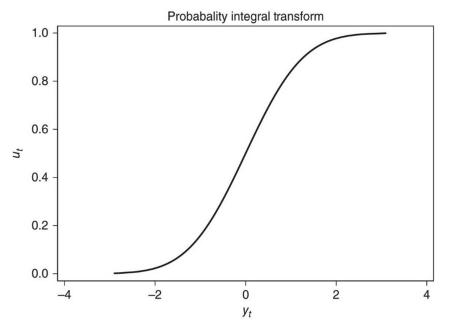
\includegraphics[width=10cm]{pics/probability integral transform.png}
    \caption{The probability transform showing how the time series $y_t$ is transformed into $u_t$ on the distribution $N(0,1)$.}
    \label{fig: PIT}
\end{figure}

In the figure below we see the different cases where the forecast is misspecified. In panel (b) we see that our mean is actually 0.5, therefore our true distribution is $N(0.5,1)$ but the forecast distribution used in the probability integral transform is $N(0,1)$. The histogram exhibits a positive slope reflecting the fact that larger values of $u_t$ and hence $y_t$ have a relatively higher probability of occurrence than smaller values of $u_t$ and $y_t$.

Panel (c) shows the effects of misspecifying the variance of the forecast distribution. If our true data-generating process is an $N(0,2)$ distribution, but again we use a forecast distribution in the PIT of $N(0,1)$ we see this U-shaped distribution. Intuitively, this is because large positive and negative values have a higher probability of occurring than are predicted by the $N(0,1)$ distribution.

\begin{figure}[h]
    \centering
    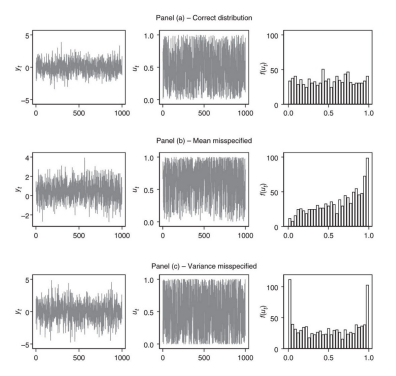
\includegraphics[width=10cm]{pics/PIT misspecification.png}
    \caption{Simulated time series to show the effects of misspecification using the probability integral transform. In panel (a) there is no misspecification, while panels (b) and (c) demonstrate the effect of misspecification in the mean and variance of the distribution, respectively.}
    \label{fig:effects of misspecification PIT}
\end{figure}
\newpage

\subsection{Regression Model Forecasts}

A simple framework for using explanatory variables in forecasting exercises is the linear regression model:
\[ y_t = \beta_0 + \beta_1 x_t + u_t,\]
where $y_t$ is the dependent variable, $x_t$ is the explanatory variable, $u_t$ is a disturbance term and the sample period is $t=1,2,\ldots,T$.

This means that the model at $T+1$ is:
\[ y_{T+1} = \beta_0 + \beta_1 x_{T+1} + u_{T+1},\]
however, we do not observe $x_{T+1}$. We can specify a time series model for $x_t$ and use this model to generate forecasts of future values $x_{T+H}$ by means of the methods discussed previously. Let's assume we propose an AR(2) model for $x_t$, the overall model then becomes a bivariate system of equations of the form
\begin{equation}
\begin{aligned}
& y_t=\beta_0+\beta_1 x_t+u_t \\
& x_t=\phi_0+\phi_1 x_{t-1}+\phi_2 x_{t-2}+v_t
\end{aligned}
\end{equation}
To generate the first forecast at time $T+1$, the system if equations is written as:
\begin{equation}
\begin{aligned}
& y_{T+1}=\beta_0+\beta_1 x_{T+1}+u_{T+1} \\
& x_{T+1}=\phi_0+\phi_1 x_T+\phi_2 x_{T-1}+v_{T+1} .
\end{aligned}
\end{equation}
Replacing the unknown parameters with estimates and the unknown equation errors with expectations (zero) yields the predictive system:
\begin{equation}
\begin{aligned}
& \widehat{y}_{T+1}=\widehat{\beta}_0+\widehat{\beta}_1 \widehat{x}_{T+1} \\
& \widehat{x}_{T+1}=\widehat{\phi}_0+\widehat{\phi}_1 x_T+\widehat{\phi}_2 x_{T-1} .
\end{aligned}
\end{equation}

So, we must first generate a forecast for $\hat{x}_{T+1}$ and then use this to forecast $\hat{y}_{T+1}$. This can be performed in a single step:
\begin{equation}
\begin{aligned}
\widehat{y}_{T+1} & =\widehat{\beta}_0+\widehat{\beta}_1\left(\widehat{\phi}_0+\widehat{\phi}_1 X_T+\widehat{\phi}_2 X_{T-1}\right) \\
& =\widehat{\beta}_0+\widehat{\beta}_1 \widehat{\phi}_0+\widehat{\beta}_1 \widehat{\phi}_1 x_T+\widehat{\beta}_1 \widehat{\phi}_2 x_{T-1} .
\end{aligned}
\end{equation}




\newpage
\section{Maximum Likelihood}
\textbf{Chapter 10}

\subsection{Motivation for MLE}

We have only used forms of the OLS estimator so far. Tis minimises the sum of squared errors when solving for the parameters. Under the Central Limit Theorem assumptions, the OLS is optimal.

\subsubsection{CLM assumptions with finite TS data}

\begin{equation}
y_t=\beta_0+\beta_1 x_{t 1}+\beta_2 x_{t 2}+\ldots+\beta_k x_{t k}+u_t, t=1, \ldots, n .
\end{equation}

\begin{itemize}
    \item Our equation of $y_t$ is a linear function of parameters ($\beta$s)
    \item Strict Exogeneity: $E(u_t|\boldsymbol{X})=0$
    \item Homoskedasticity: $var(u_t|\boldsymbol{X})=\sigma^2$
    \item No serial Correlation: $corr(u_t,u_s|\boldsymbol{X})=0$
    \item Normality: $u_t$ is independent of $\boldsymbol{X}$ and i.i.d $\sim N(0,\sigma^2)$.
\end{itemize}


Exogeneity implies that $x_{t1}, x_{t2}, \ldots, x_{tk}$ are "foxed" in repeated sampling, meaning they are treated as values and not random variables. They contain no information about the $\beta$s such that their distributions can be ignored. $\beta_j$ is the partial effect of $x_{tj}$ on $y_t$. It measures the change in the conditional mean value of $y_t$, $E(y_t|x_{t1},x_{t2}, \ldots)$ per unit change in $x_{tj}$, holding the other explanatory variables constant.

\subsubsection{Violations}

However, these assumptions often do not hold.
\begin{itemize}
    \item Linearity in parameters do not always hold (VECM)
    \item Fixed regressors are unrealistic (simultaneity, dynamics)
    \item Spherical errors are rare (heteroskedasticity, autocorrelation)
    \item Normality (continuity) is very restrictive: binary (discrete choice), integer-valued (count data), strictly positive data, skewed etc.
\end{itemize}

We need a more general inferential procedure that is valid for more general data types and, under less restrictive and more empirically realistic assumptions.

\subsubsection{Maximum Likelihood Estimation}

\begin{definition}
    \textbf{Maximum Likelihood estimation}:
    \begin{itemize}
        \item relies on the probability distribution of data
        \item Obtained by finding the value of the unknown parameter vector that is \textit{most likely} to have generated the observed data
    \end{itemize}
\end{definition}
\begin{note}
    Most likely: probabilistic sense. The maximum likelihood estimator is that value of the parameter which \textbf{maximises the probability density function} of the data, given the actual observations.
\end{note}

This method requires that the probability distribution of the stochastic process generating the observed data be fully specified. This requirement is more stringent than what is needed for other estimators such as OLS, IV, GMM.

\paragraph{Why MLE?}\mbox{}

MLE is attractive because the maximum likelihood estimator \hl{possesses a number of highly desirable large-sample properties under very general conditions}.

The method is often used under the presumption of a convenient probabilistic distribution such as the normal, in this case, the method is sometimes referred to as Gaussian estimation or pseudo-maximum likelihood.

\subsection{Distributions in Finance}

\subsubsection{Normality}
A common assumption is that the returns, $r_t$, on an asset are normally distributed with mean $\mu$ and variance $\sigma^2$:
\begin{equation}
\label{Normal distribution}
f\left(r_t ; \mu, \sigma^2\right)=\frac{1}{\sqrt{2 \pi \sigma^2}} \exp \left[-\frac{\left(r_t-\mu\right)^2}{2 \sigma^2}\right], \quad \text { or } \quad r_t \sim N\left(\mu, \sigma^2\right)
\end{equation}
\begin{note}
    This normality equation is specified in terms of the constant mean model
\end{note}

We use two important models that assume normality.

\paragraph{Constant Mean Model} \mbox{}
\begin{equation}
    \label{constant mean model}
    r_t = \mu + u_t, \qquad u_t \sim iid N(0,\sigma^2).
\end{equation}
From the distributional assumption of the error term we are assuming the distribution of $r_t$ to be normal, that is
\begin{equation}
f\left(r_t ; \theta\right)=\frac{1}{\sqrt{2 \pi \sigma^2}} \exp \left[-\frac{\left(r_t-\mu\right)^2}{2 \sigma^2}\right]
\end{equation}
where $\theta = \{\mu, \sigma^2\}$ is the parameter vector.

\paragraph{CAPM} \mbox{}

\begin{equation}
r_t-r_{f t}=\alpha+\beta\left(r_{m t}-r_{f t}\right)+u_t, \quad u_t \sim i i d N\left(0, \sigma^2\right) .
\end{equation}
In this case, the distribution of $r_t$ is:
\begin{equation}
f\left(r_t \mid r_{m t}, r_{t t} ; \theta\right)=\frac{1}{\sqrt{2 \pi \sigma^2}} \exp \left[-\frac{\left(r_t-r_{t t}-\alpha-\beta\left(r_{m t}-r_{f t}\right)\right)^2}{2 \sigma^2}\right]
\end{equation}
with parameter vector $\theta=\{\alpha,\beta,\sigma^2\}$.

\paragraph{Non-normality} \mbox{}

As we know many financial return series display leptokurtic distributions. That is the normal distribution assumption does not capture the peakedness of the distribution, tending to underestimate the observed mode.

\subsubsection{t-distribution}

We often replace the assumption of normality with the assumption that returns follow a $t$ distribution, whose probability density is given by:

\begin{equation}
f\left(r_t ; \mu, \sigma^2, \nu\right)=\frac{\Gamma\left(\frac{\nu+1}{2}\right)}{\sqrt{\pi \sigma^2 \nu} \Gamma\left(\frac{\nu}{2}\right)}\left(1+\frac{\left(r_t-\mu\right)^2}{\sigma^2 \nu}\right)^{-\left(\frac{\nu+1}{2}\right)}
\end{equation}
where $\nu$ represents the degrees of freedom parameter and $\Gamma(.)$ is the gamma function. $\nu$ allows for additional flexibility in modelling empirical distributions.

\begin{note}
    As $\nu\rightarrow\infty$ the $t$ distribution becomes the normal distribution.
\end{note}

\subsubsection{Lognormal Distributions}

When we use log returns (like normal) we assume that $r_t$ is normally distributed with mean $\mu$ and variance $\sigma^2$ implies that $P_t$, conditional on the lagged price $P_{t-1}$ is \textbf{log normally distributed} with density:

\begin{equation}
f\left(P_t \mid P_{t-1} ; \mu, \sigma^2\right)=\frac{1}{\sqrt{2 \pi \sigma^2} P_t} \exp \left[-\frac{\left(\log P_t-\left(\mu+\log P_{t-1}\right)\right)^2}{2 \sigma^2}\right] .
\end{equation}

\begin{note}
    An important feature of this distribution is that it is defined only over the non-negative region. The support of the distribution is therefore said to be the non-negative part of the real line.

    This usually results in the distribution exhibiting positive skewness with a long right hand tail.
\end{note}

\begin{figure}[h]
    \centering
    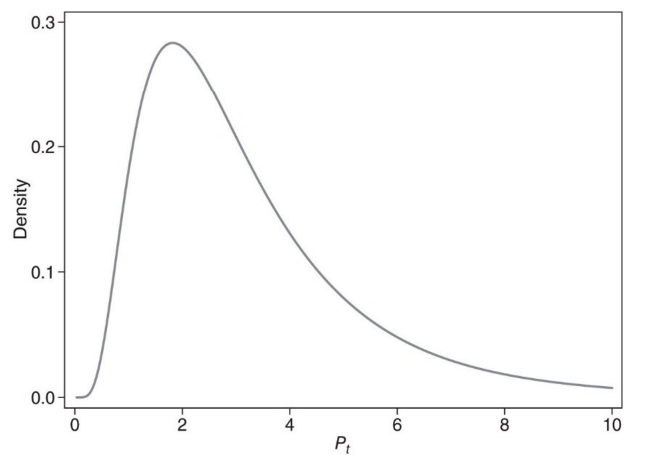
\includegraphics[width=10cm]{pics/lognormal dist.png}
    \caption{A plot of the lognormal distribution for equity prices $\mu = 1, \sigma^2 = 0.4, P_{t-1} = 1$}
    \label{fig:lognormal distribution}
\end{figure}

\begin{example}
    Simple gross returns on an asset: $R_{gt}$

    Log-returns are defined as:
\begin{equation}
r_t=\log \left(\frac{P_t}{P_{t-1}}\right)=\log \left(1+\frac{P_t-P_{t-1}}{P_{t-1}}\right)=\log \left(1+R_t\right)=\log \left(R_{g t}\right)
\end{equation}

If $r_t$ is normally distributed with mean $\mu$ and variance $\sigma^2$, then $R_{gt} = P_t/P_{t-1}$ is lognormally distributed with density
\begin{equation}
f\left(R_{g t} ; \mu, \sigma^2\right)=\frac{1}{\sqrt{2 \pi \sigma^2} R_{g t}} \exp \left[-\frac{\left(\log R_{g t}-\mu\right)^2}{2 \sigma^2}\right]
\end{equation}
\end{example}

\begin{example}
    Black-Scholes Options Pricing Model:
    We assume that price $P_t$ of an asset is determined by the following equation
    \[log P_t - log(P_{t-1} = \mu + u_t, \qquad u_t \sim N(0,\sigma^2),\]
    which implies that log prices follow a Gaussian random walk with drift. The use of cumulative normal distribution functions then arises naturally in computing the option price formula and follows directly from this lognormality assumption.
\end{example}

\subsubsection{Gamma Distribution}

The Gamma distribution with parameter vectir $\theta = \{\alpha,\beta\}$ and density
\begin{equation}
f\left(y_t ; \theta\right)=\frac{\alpha^\beta}{\Gamma(\beta)} y_t^{\beta-1} e^{-\alpha y_t}
\end{equation}
where, $\alpha$ and $\beta$ are called the shape and rate parameters of the distribution.

\begin{figure}[h]
    \centering
    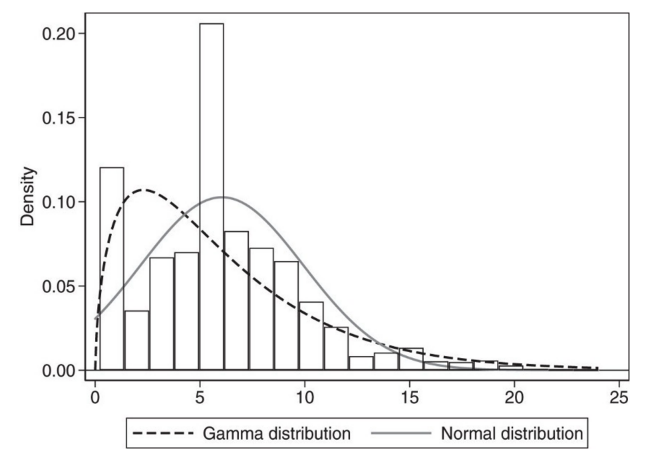
\includegraphics[width=10cm]{pics/gamma vs normal dist.png}
    \caption{Histogram of daily Eurodollar rate superimposed on the histogram are plots of the best-fitting normal and gamma distributions.}
    \label{fig:gamma vs normal}
\end{figure}

\subsubsection{Weibull and Exponential Distributions}

The Weibull distribution has a parameter vector $\theta = \{\alpha,\beta\}$ and density
\begin{equation}
f\left(y_t ; \alpha, \beta\right)=\alpha \beta y_t^{\beta-1} e^{-\alpha y_t^\beta}, \quad \alpha, \beta>0
\end{equation}

When $\beta=1$ we have an exponential distribution:
\[f(y_t;\alpha) = \alpha e^{-\alpha y_t}, \qquad \alpha>0\]

\subsection{Estimation by Maximum Likelihood (10.2)}

The log likelihood function for a parameter vector $\theta$ (which is to be estimated from a given sample of $T$ observations $\{y_1, y_2, \ldots, y_T\}$) is constructed as follows:

\begin{definition}
        The log likelihood function:
        \begin{enumerate}
            \item i.i.d observations:
            \begin{equation}
                \log L(\theta)=\frac{1}{T} \sum_{t=1}^T \log f\left(y_t ; \theta\right)
            \end{equation}
            \item Non-identically distributed observations:
            \begin{equation}
                \log L(\theta)=\frac{1}{T} \sum_{t=1}^T \log f\left(y_t \mid x_t ; \theta\right)
            \end{equation}
            \begin{note}
                This is now conditional on $x_t$
            \end{note}
            \item Dependently Distributed Observations
            \begin{equation}
                \log L(\theta)=\frac{1}{T-1} \sum_{t=2}^T \log f\left(y_t \mid y_{t-1} ; \theta\right)
            \end{equation}
            \begin{note}
                This is now conditional on lagged dependent variable. Also, divided by T-1 due to the lag we have one less observation.
            \end{note}
            \item Dependent and non-identically distributed observations:
            \begin{equation}
                \log L(\theta)=\frac{1}{T-1} \sum_{t=2}^T \log f\left(y_t \mid x_t, y_{t-1} ; \theta\right)
            \end{equation}
            \begin{note}
                conditional on both $x_t$ and $y_{t-1}$. also divided by T-1 due to the lag.
            \end{note}
        \end{enumerate}
\end{definition}

\subsubsection{The Maximum Likelihood Estimator (MLE)}

The maximum likelihood estimator of $\theta$, denoted $\hat{\theta}$, satisfies the zero gradient condition. Therefore, is found by taking the first derivative of our log-likelihood function with respect to $\theta$ and solving for the 0. \textit{The first derivative w.r.t $\theta$ is called the gradient} and denoted $G(\theta)$.

$\hat{\theta}$ is the value that maximises the likelihood function $L(\theta)$ and may be interpreted as the value of $\theta$ which is \textbf{most likely} to have generated the observed data. 

\paragraph{Second Order Condition} \mbox{}

The condition required for the maximum likelihood estimator to maximise $log L(\theta)$ is that the Hessian (second derivative of $log L(\theta)$) be negative at $\hat{\theta}$.

\begin{equation}
H(\widehat{\theta})=\left.\frac{\partial^2 \log L(\theta)}{\partial \theta \partial \theta^{\prime}}\right|_{\theta=\widehat{\theta}}<0 .
\end{equation}

This is also known as the second-order condition (SOC).

\subsubsection{Model of Duration of Trades}

The duration model of trades, $y_t$, is given by the exponential distribution:
\[f(y_t;\alpha_t) = \alpha e^{-\alpha y_t}, \qquad \alpha>0\]
where observations of $y_t$ are iid. Because of this, we know $log L(\theta)$ follows the first case.

Below we see the distribution of time between trades graphically,
\begin{figure}[h]
    \centering
    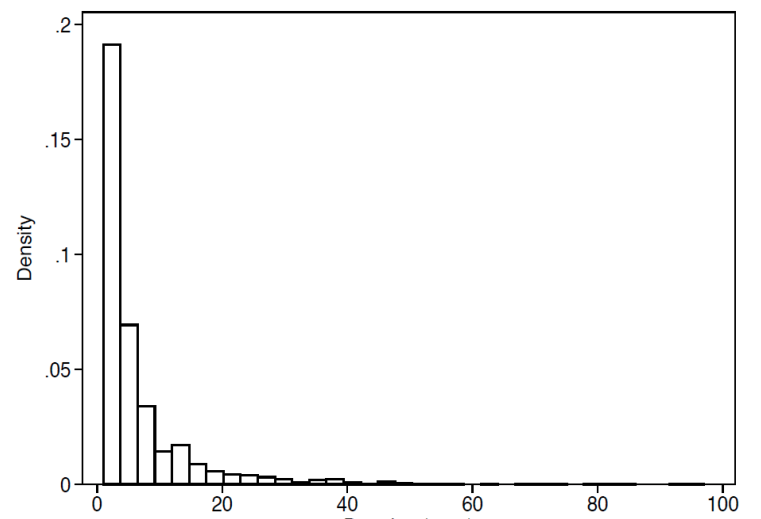
\includegraphics[width=10cm]{pics/duration between trades.png}
    \caption{Duration (secs) between trades}
    \label{fig:duration between trades}
\end{figure}

We have our log-likelihood function:
\begin{equation}
\begin{aligned}
\log L(\theta) & =\frac{1}{T} \sum_{t=1}^T \log f\left(y_t ; \theta\right)=\frac{1}{T} \sum_{t=1}^T \log \left(\theta \exp \left[-\theta y_t\right]\right) \\
& =\frac{1}{T} \sum_{t=1}^T \log \theta-\frac{1}{T} \sum_{t=1}^T \theta y_t=\log \theta-\theta \frac{1}{T} \sum_{t=1}^T y_t
\end{aligned}
\end{equation}

From this we can find the gradient and by setting our gradient to 0 we get:

\begin{equation}
G(\theta)=\frac{d \log L(\theta)}{d \theta}=\frac{1}{\theta}-\frac{1}{T} \sum_{t=1}^T y_t \Rightarrow \frac{1}{\widehat{\theta}}-\frac{1}{T} \sum_{t=1}^T y_t=0 .
\end{equation}

Solving for $\hat{\theta}$ yields the maximum likelihood estimator
\[\hat{\theta} = \dfrac{T}{\sum_{t=1}^T y_t} = \dfrac{1}{\bar{y}}\]
which is the reciprocal of the sample mean of the durations data.

\subsubsection{Constant Mean Model}
Our constant mean model of returns is:
\[r_t = \mu + u_t, \qquad u_t \sim iid N(0,\sigma^2)\]

Although we have made a distributional assumption about the disturbance term we can easily deduce the distribution of $r_t$ to be
\begin{equation}
u_t=\left(r_t-\mu\right) \sim i i d N\left(0, \sigma^2\right) \Rightarrow r_t \sim \operatorname{iid} N\left(\mu, \sigma^2\right)
\end{equation}

so we know that the sample data, $r_t$, are independent drawings from a normal distribution with mean $\mu$ and variance $\sigma^2$. The distribution of $r_t$ is therefore given by

\begin{equation}
f\left(r_t ; \theta\right)=\frac{1}{\sqrt{2 \pi \sigma^2}} \exp \left[-\frac{\left(r_t-\mu\right)^2}{2 \sigma^2}\right]
\end{equation}
with parameter vector $\theta = \{\mu, \sigma^2\}$. We know $r_t$ is iid, therefore the log-likelihood function follows case 1 and has the form:

\begin{equation}
\begin{aligned}
\log L(\theta) & =\frac{1}{T} \sum_{t=1}^T \log f\left(r_t ; \theta\right)=\frac{1}{T} \sum_{t=1}^T \log \left(\frac{1}{\sqrt{2 \pi \sigma^2}} \exp \left[-\frac{\left(r_t-\mu\right)^2}{2 \sigma^2}\right]\right) \\
& =-\frac{1}{2} \log 2 \pi-\frac{1}{2} \log \sigma^2-\frac{1}{2 \sigma^2} \frac{1}{T} \sum_{t=1}^T\left(r_t-\mu\right)^2
\end{aligned}
\end{equation}

The gradient vector is therefore
\begin{equation}
G(\theta)=\left[\begin{array}{c}
\frac{\partial \log L(\theta)}{\partial \mu} \\
\frac{\partial \log L(\theta)}{\partial \sigma^2}
\end{array}\right]=\left[\begin{array}{c}
\frac{1}{\sigma^2 T} \sum_{t=1}^T\left(r_t-\mu\right) \\
-\frac{1}{2 \sigma^2}+\frac{1}{2 \sigma^4 T} \sum_{t=1}^T\left(r_t-\mu\right)^2
\end{array}\right] .
\end{equation}

So, the maximum likelihood estimator is found by setting $G(\hat{\theta}) = 0$ which requires solving the two equations

\begin{equation}
\begin{array}{r}
\frac{1}{\widehat{\sigma}^2 T} \sum_{t=1}^T\left(r_t-\widehat{\mu}\right)=0 \\
-\frac{1}{2 \widehat{\sigma}^2}+\frac{1}{2 \widehat{\sigma}^4 T} \sum_{t=1}^T\left(r_t-\widehat{\mu}\right)^2=0
\end{array}
\end{equation}
for $\hat{\mu}$ and $\hat{\sigma}^2$.

\paragraph{Solving Mean} \mbox{}

Solving our first equation in $G(\hat{\theta})$ for $\mu$:
\begin{equation}
\frac{1}{\widehat{\sigma}^2 T} \sum_{t=1}^T\left(r_t-\widehat{\mu}\right)=\sum_{t=1}^T\left(r_t-\widehat{\mu}\right)=\sum_{t=1}^T r_t-T \widehat{\mu}=0
\end{equation}
so the maximum likelihood estimator is given by the sample mean of $r_t$

\begin{equation}
T \widehat{\mu}=\sum_{t=1}^T r_t \Rightarrow \widehat{\mu}=\frac{1}{T} \sum_{t=1}^T r_t=\bar{y}
\end{equation}

\paragraph{Solving Variance} \mbox{}

Solving for $\sigma^2$ using the second equation in $G(\hat{\theta})$ gives

\begin{equation}
-\frac{1}{2 \widehat{\sigma}^2}+\frac{1}{2 \widehat{\sigma}^4 T} \sum_{t=1}^T\left(r_t-\widehat{\mu}\right)^2=0
\end{equation}

which leads to the solution 

\begin{equation}
\widehat{\sigma}^2=\frac{1}{T} \sum_{t=1}^T\left(r_t-\widehat{\mu}\right)^2
\end{equation}
This expression is the sample variance of $r_t$. Differentiating $G(\theta)$ with respect to $\theta$ yields the (2x2) Hessian Matrix:

\begin{equation}
H(\theta)=\left[\begin{array}{cc}
-\frac{1}{\sigma^2} & -\frac{1}{\sigma^4 T} \sum_{t=1}^T\left(r_t-\mu\right) \\
-\frac{1}{\sigma^4 T} \sum_{t=1}^T\left(r_t-\mu\right) & \frac{1}{2 \sigma^4}-\frac{1}{\sigma^6 T} \sum_{t=1}^T\left(r_t-\mu\right)^2
\end{array}\right] .
\end{equation}

and then evaluating the matrix at $\hat{\theta}$

\begin{equation}
H(\widehat{\theta})=\left[\begin{array}{ll}
H_{11} & H_{12} \\
H_{21} & H_{22}
\end{array}\right]=\left[\begin{array}{cc}
-\frac{1}{\widehat{\sigma}^2} & 0 \\
0 & -\frac{1}{2 \widehat{\sigma}^4}
\end{array}\right],
\end{equation}

The relevant SOC for the maximum are satisfied because the second derivative is negative
\begin{equation}
\begin{aligned}
H_{11} & =-\frac{1}{\widehat{\sigma}^2}<0 \\
H_{11} H_{22}-H_{12} H_{21} & =\left(-\frac{1}{\widehat{\sigma}^2}\right)\left(-\frac{1}{2 \widehat{\sigma}^4}\right)-(0)(0)=\frac{1}{2 \widehat{\sigma}^6}>0 .
\end{aligned}
\end{equation}

\subsubsection{Numerical Methods}

In many financial econometric applications, the system of FOC $G(\hat{\theta}) = 0$ for maximum likelihood does \textbf{not} have an analytical answer. In these cases, we need an alternative method to locate the maximum of the likelihood function. This is usually iterative but can also involve systematic searching over a grid of possible values,

\paragraph{Iterative Methods} work from some starting value for $\theta$, denoted $\theta_{(0)}$, and at each stage produce a new potential value $\theta_{(k)}$ proceeding sequentially until convergence.

Convergence is deemed to occur when $G(\hat{\theta}_{(k)}) \approx 0$ and $\hat{\theta}_{(k+1} \approx \hat{\theta}_{(k}$ up to some specified level of tolerance in terms of significant figures. This is called \textbf{numerical optimisation}.

\subsubsection{Robust CAPM}

Let $y_t = r_t - r_{ft}$ be the excess return on the asset and $x_t = r_{mt} - r_{ft}$ be the excess return on the market, then
\[y_t = \alpha + \beta x_t + u_t, \qquad u_t \sim St(0,\sigma^2,\nu)\]

and $St(0,\sigma^2,\nu)$ represents a standardised form of the $t$ distribution. The distribution of the observations $y_t$ is

\begin{equation}
f\left(y_t \mid x_t ; \theta\right)=\frac{\Gamma\left(\frac{\nu+1}{2}\right)}{\sqrt{\pi \sigma^2(\nu-2)} \Gamma\left(\frac{\nu}{2}\right)}\left(1+\frac{\left(y_t-\alpha-\beta x_t\right)^2}{\sigma^2(\nu-2)}\right)^{-\left(\frac{\nu+1}{2}\right)}
\end{equation}

We can see that this is a case of non-identically distributed observations, so case 2, and the log-likelihood function based on this fact has the form

\begin{equation}
\begin{aligned}
\log L(\theta) & =\frac{1}{T} \sum_{t=1}^T \log f\left(y_t \mid x_t ; \theta\right)=\log \Gamma\left(\frac{\nu+1}{2}\right)-\frac{1}{2} \log \sigma^2-\frac{1}{2} \log (\pi(\nu-2)) \\
& -\log \Gamma\left(\frac{\nu}{2}\right)-\left(\frac{\nu+1}{2}\right) \frac{1}{T} \sum_{t=1}^T \log \left(1+\frac{\left(y_t-\alpha-\beta x_t\right)^2}{\sigma^2(\nu-2)}\right) .
\end{aligned}
\end{equation}

We can see that the expression for the log-likelihood function is nonlinear in the parameters. Therefore, a numerical approach is adopted to compute the maximum likelihood estimator, $\hat{\theta}$.


\subsubsection{Interest Rate Model (Vasicek (1977))}

The discrete time model of the interest rate, $r_t$, proposed by Vasicek (1977) is
\[r_t = \alpha + \rho r_{t-1} + u_t, \qquad u_t \sim iid N(0,\sigma^2)\]

The resulting distribution of $r_t$ with parameter vector $\theta = \{\alpha, \rho, \sigma^2\}$ is given by

\begin{equation}
f\left(r_t \mid r_{t-1} ; \alpha, \rho, \sigma^2\right)=\frac{1}{\sqrt{2 \pi \sigma^2}} \exp \left[-\frac{\left(r_t-\alpha-\rho r_{t-1}\right)^2}{2 \sigma^2}\right]
\end{equation}

The log-likelihood $\log L(\theta)$ is based on case 3 (dependently distributed observations), so we have:

\begin{equation}
\log L\left(\alpha, \rho, \sigma^2\right)=-\frac{1}{2} \log 2 \pi-\frac{1}{2} \log \sigma^2-\frac{1}{2 \sigma^2} \frac{1}{T-1} \sum_{t=2}^T\left(r_t-\alpha-\rho r_{t-1}\right)^2
\end{equation}

The maximum likelihood estimators are therefore given by the following explicit formulae:

\begin{equation}
\begin{aligned}
\widehat{\alpha} & =\bar{r}_t-\widehat{\rho} \bar{r}_{t-1} \\
\widehat{\rho} & =\frac{\sum_{t=2}^T\left(r_t-\bar{r}_t\right)\left(r_{t-1}-\bar{r}_{t-1}\right)}{\sum_{t=2}^T\left(r_{t-1}-\bar{r}_{t-1}\right)^2} \\
\widehat{\sigma}^2 & =\frac{1}{T-1} \sum_{t=2}^T\left(r_t-\widehat{\alpha}-\widehat{\rho} r_{t-1}\right)^2 .
\end{aligned}
\end{equation}


\subsubsection{Standard Errors}

Standard errors of $\hat{\theta}$ are estimated by the square roots of the diagonal elements of the covariance matrix of the maximum likelihood estimator. The covariance matrix of $\hat{\theta}$ takes the following asymptotic form

\begin{equation}
E\left[\left(\widehat{\theta}-\theta_0\right)\left(\widehat{\theta}-\theta_0\right)^{\prime}\right] \stackrel{a}{\sim} \dfrac{1}{T}\Omega\left(\theta_0\right)
\end{equation}

\paragraph{Estimating the Covariance Matrix} \mbox{}

\begin{procedure}
We have two common choices for estimating the asymptotic covariance matrix $\Omega(\theta_0)$ are:
    \begin{enumerate}
        \item An estimate based on the Hessian Matrix
        \[\Omega(\hat{\theta}) = -H(\hat{\theta})^{-1},\]

        \item An estimate based on the Outer Product of Gradients (OPG) Matrix
        \begin{equation}
\Omega(\widehat{\theta})=J(\widehat{\theta})^{-1}, \quad \text { where } \quad J(\widehat{\theta})=\left.\frac{1}{T} \sum_{t=1}^T \frac{\partial \log f\left(y_t ; \theta\right)}{\partial \theta} \frac{\partial \log f\left(y_t ; \theta\right)}{\partial \theta^{\prime}}\right|_{\theta=\widehat{\theta}} .
\end{equation}
    \end{enumerate}

    The covariance matrix of $\hat{\theta}$ can therefore be estimated via two formulae:
    
    \begin{equation}
        cov(\hat{\theta}_T) = \Biggl\{ \begin{array}{cc}
            -\dfrac{1}{T}H(\hat{\theta})^{-1} & \text{Hessian}  \\
             \dfrac{1}{T}J(\hat{\theta})^{-1}& \text{Outer product of gradients} 
        \end{array}
    \end{equation}
    Standard errors of $\hat{\theta}$ are given by the square roots of the diagonal elements of the matrix.
\end{procedure}

\subsection{Properties of MLE}

\begin{shaded}
    Under regularity conditions which are quite weak, maximum likelihood estimators have the following properties:
    \begin{enumerate}
        \item \textbf{Consistency}
        \[plim(\hat{\theta}_T) = \theta_0.\]

        \item \textbf{Efficiency}

        Asymptotic efficiency concerns the degree of dispersion (scatter or variation) of $\hat{\theta}_T$ around $\theta_0$ as the sample size $T$ increases. \textit{An important asymptotic property of the maximum likelihood estimator is that this estimator is more efficient than any other estimator}.

        \item \textbf{Asymptotic Normality}

        The asymptotic distribution of $\hat{\theta}_T$ is given by

        \begin{equation}
            \widehat{\theta}_T \stackrel{a}{\sim} N\left(\theta_0, \frac{1}{T} \Omega\left(\theta_0\right)\right), \quad \sqrt{T}\left(\widehat{\theta}_T-\theta_0\right) \stackrel{d}{\longrightarrow} N\left(0, \Omega\left(\theta_0\right)\right) .
        \end{equation}

        \begin{note}
            The first expression shows the asymptotic approximation to the finite sample distribution of $\hat{\theta}_T$. The second expression shows the precise form of the limiting distribution as $T\rightarrow\infty$.
        \end{note}

        \item \textbf{Invariance}

        For any nonlinear function $\tau(.)$, the maximum likelihood estimator of $\tau(\theta_0)$ is given by $\tau(\hat{\theta}_T)$.
    \end{enumerate}
\end{shaded}

\subsubsection{Misspecification}

We have assumed so far that the corresponding likelihood functions are all founded on the assumption that the models are specified correctly. Some of the properties of ML continue to hold under a model and likelihood misspecification.
\begin{example}
    For a misspecified model, it may be possible to estimate a subset of parameters for which consistency and asymptotic normality still hold even when the log-likelihood function for these models is misspecified.
\end{example}

\begin{definition}
    \textbf{Quasi Maximum Likelihood}: When the likelihood is constructed under misspecification, it is called the quasi likelihood. The log likelihood is the quasi-log likelihood and the estimator is known as a quasi maximum likelihood estimator (QMLE).
\end{definition}

under general conditions, the asymptotic distribution of the QMLE, written as $(\hat{\theta}_Q)$, has the form

\begin{equation}
\sqrt{T}\left(\hat{\theta}_Q-\theta_0\right) \stackrel{d}{\rightarrow} N\left(0, \Omega_Q\right)
\end{equation}

whose asymptotic variance $\Omega_Q$ depends on the type of misspecification introduced into the model and likelihood.

\subsubsection{Types of Misspecification}

Three types of misspecification lead to different estimates of asymptotic variance $\Omega_Q$. Define $x_t = (x_{1t})^\prime$.


\paragraph{Nonnormality in the linear model} \mbox{}

Supposed
\[y_t = \alpha + \beta x_{1t} + u_t, \qquad u_t \sim N(0,\sigma^2_u).\]

Given our definition of $x_t$, under nonnormality of $u_t$,

\begin{equation}
\frac{1}{T} \widehat{\Omega}_Q=\frac{\widehat{\sigma}_U^2}{T}\left(\frac{1}{T} \sum_{t=1}^T x_t x_t^{\prime}\right)^{-1}
\end{equation}

\paragraph{heteroskedasticity}\mbox{}

In the presence of heteroskedasticity in $u_t$,
\begin{equation}
\frac{1}{T} \widehat{\Omega}_Q=\frac{1}{T}\left(\frac{1}{T} \sum_{t=1}^T x_t x_t^{\prime}\right)^{-1}\left(\frac{1}{T} \sum_{t=1}^T \widehat{u}_t^2 x_t x_t^{\prime}\right)\left(\frac{1}{T} \sum_{t=1}^T x_t x_t^{\prime}\right)^{-1}
\end{equation}

\paragraph{Autocorrelation in the linear model} \mbox{}

When $u_t$ is autocorrelated, 

\begin{equation}
\frac{1}{T} \widehat{\Omega}_Q=\frac{1}{T}\left(\frac{1}{T} \sum_{t=1}^T x_t x_t^{\prime}\right)^{-1}\left(\widehat{\Gamma}_0+\sum_{i=1}^p w_i\left(\widehat{\Gamma}_i+\widehat{\Gamma}_i^{\prime}\right)\right)\left(\frac{1}{T} \sum_{t=1}^T x_t x_t^{\prime}\right)^{-1}
\end{equation}
with 
\begin{equation}
\widehat{\Gamma}_i=\frac{1}{T} \sum_{t=i+1}^T \widehat{u}_t \widehat{u}_{t-i} x_t x_{t-i}^{\prime}, i=0,1,2, \cdots
\end{equation}

\newpage

\subsection{Testing MLE}

the likelihood function gives us a simple and intuitive approach to inference, the most common form of which is to \textbf{test whether the parameter of the model has a certain hypothesised value}, $\theta_0$.

If this value differs from the maximum likelihood estimate $\hat{\theta}$, then by virtue of the construction of $\hat{\theta}$ the hypothesised value $\theta_0$ must correspond to a lower value of the log likelihood function.

\paragraph{Simple Example} \mbox{}

The simplest version of the null and alternative hypotheses to be tested may be stated in terms of the \textbf{full parameter vector} $\theta$ in the form
\[H_0: \theta = \theta_0, \qquad H_1: \theta \neq \theta_0.\]

The crucial statistical question if how significant the decrease in likelihood is in moving between the two values.

There are three common tests for such hypotheses.
\begin{itemize}
    \item Likelihood ratio test (LR)
    \item Wald Test (WD)
    \item Lagrange Multiplier Test (LM)
\end{itemize}
They vary depending on whether the test takes place under the null, alternative or both hypotheses.

\paragraph{Estimators for the test}\mbox{}

Define the following estimators
\begin{align*}
    &\hat{\theta}_0: \text{ parameters estimated under the restrictions of the null hypothesis } H_0 \\
    & \hat{\theta}_1: \text{ parameters estimated with no such restrictions } H_1.
\end{align*}

\paragraph{Test Statistics} \mbox{}

The following forms symbolise the construction of these three tests, which involve the use of the restricted and unrestricted estimates of $\theta$.

\begin{equation}
    \begin{array}{ccc}
    \text{Likelihood Ratio:} & LR= & -2 T\left(\log L\left(\widehat{\theta}_0\right)-\log L\left(\widehat{\theta}_1\right)\right) \\
    \text{Wald:} & WD =& T\left[\widehat{\theta}_1-\widehat{\theta}_0\right]^{\prime}\left[\Omega\left(\widehat{\theta}_1\right)\right]^{-1}\left[\widehat{\theta}_1-\widehat{\theta}_0\right] \\
    \text{Lagrange Multiplier:}& LM=& T G\left(\widehat{\theta}_0\right)^{\prime}\left[\Omega\left(\widehat{\theta}_0\right)\right] G\left(\widehat{\theta}_0\right)
\end{array}
\end{equation}


\begin{definition}
    Comparison of tests:
    \begin{itemize}
        \item The LR test involves estimation of the model under \textbf{both null and alternative hypotheses}
        \item In certain circumstances, the WD test involves estimation under the \textbf{alternative hypothesis alone}
        \item The LM test involves estimation under the \textbf{null hypothesis alone}.
        \item All three:
        In large samples, they are distributed as $\chi^2_M$, where $M$ is the number of restrictions associated with the null hypothesis.
    \end{itemize}
\end{definition}

\begin{shaded}
    \paragraph{Intuition:} \mbox{}

    \textbf{Likelihood ratio test:} Measures the distance between the value of the log-likelihood under the null hypothesis and the alternative hypothesis. That is comparing $\log L(\hat{\theta}_0)$ and $\log L(\hat{\theta}_1)$.

    \textbf{Wald test:} Measures the distance between the parameter estimate under the alternative $\hat{\theta}_1$ and the value of the parameter under the null, $\theta_0$, weighted by the inverse of the covariance matrix of the estimate evaluated under the alternative hypothesis $\Omega(\hat{\theta}_1)$.
    \begin{note}
        We are comparing an estimated value with a hypothesised value.
    \end{note}

    \textbf{Lagrange Multiplier test:} Measures the distance between the gradient of the log-likelihood function under the null and under the alternative, that is comparing $G(\hat{\theta}_0)$ and $G(\hat{\theta}_1)$
    \begin{note}
        By virtue of the optimising property of the unrestricted maximum likelihood estimator, $G(\hat{\theta}_1) = 0$
    \end{note}
\end{shaded}

\paragraph{More on the LM test}\mbox{}

An alternative form of the LM statistic which is convenient for a broad class of models is

\begin{equation}
\begin{aligned}
L M & =T\left(\frac{1}{T} \sum_{t=1}^T g_t\right)^{\prime} \frac{1}{T}\left(\frac{1}{T} \sum_{t=1}^T g_t g_t^{\prime}\right)^{-1}\left(\frac{1}{T} \sum_{t=1}^T g_t\right) \\
& =\left(\sum_{t=1}^T g_t\right)^{\prime}\left(\sum_{t=1}^T g_t g_t^{\prime}\right)^{-1}\left(\sum_{t=1}^T g_t\right)=T R^2
\end{aligned}
\end{equation}
where $R^2$ is the coefficient of determination from regressing a vector of ones on the gradient variates $g_t$ without an intercept.

\begin{procedure}
    Computing the LM test involves:
    \begin{enumerate}
        \item Estimate the restricted model and compute $\hat{\theta}_0$
        \item Estimate the auxiliary regression where the dependent variables are the gradients in $g_t$, all evaluated at $\hat{\theta}_0$.
        \item Compute the LM stat, $TR^2$, getting $R^2$ from step 2.
    \end{enumerate}
\end{procedure}

\paragraph{Inference}
If we test the same number of restrictions using the three tests, it follows that
\begin{equation}
\operatorname{Prob}\left(\chi^2(m)>L M\right) \geq \operatorname{Prob}\left(\chi^2(m)>L R\right) \geq \operatorname{Prob}\left(\chi^2(m)>W D\right) .
\end{equation}

This means that the tests can yield conflicting conclusions, but because of the ordering we know:
\begin{itemize}
    \item If the LM test rejects the null, so will the LR and WALD tests.
    \item If the WD test fails to reject the null, then so will the LR and LM tests.
\end{itemize}

\begin{note}
    This ranking only holds when testing linear restrictions in the normal linear regression model.
\end{note}

\subsubsection{Application of our tests}

\paragraph{testing our durations model} \mbox{}

Assume now that the durations model follows the Weibull distribution
\begin{equation}
f\left(y_t ; \alpha, \beta\right)=\alpha \beta y_t^{\beta-1} e^{-\alpha y_t^\beta}, \quad \alpha, \beta>0
\end{equation}

a natural test would be to test whether we have an exponential distribution and test
\[H_0: \beta=1, \qquad H_1: \beta\neq1\]
so, under the null, the Weibull distribution reduces to the exponential distribution.

The unrestricted log likelihood is:
\begin{equation}
\log L(\theta)=\log (\alpha)+\log (\beta)+(\beta-1) \frac{1}{T} \sum_{t=1}^T \log y_t-\alpha \frac{1}{T} \sum_{t=1}^T y_t^\beta .
\end{equation}

the gradients are:
\begin{equation}
\begin{aligned}
& \frac{\partial \log L(\theta)}{\partial \alpha}=\frac{1}{\alpha}-\frac{1}{T} \sum_{t=1}^T y_t^\beta \\
& \frac{\partial \log L(\theta)}{\partial \beta}=\frac{1}{\beta}+\frac{1}{T} \sum_{t=1}^T \log y_t-\alpha \frac{1}{T} \sum_{t=1}^T \log \left(y_t\right) y_t^\beta .
\end{aligned}
\end{equation}

This means that the maximum likelihood estimator $\hat{\theta} = \{\hat{\alpha}, \hat{\beta}\}$ is the solution of

\begin{equation}
\begin{aligned}
& 0=\frac{1}{\widehat{\alpha}}-\frac{1}{T} \sum_{t=1}^T y_t^{\widehat{\beta}} \\
& 0=\frac{1}{\widehat{\beta}}+\frac{1}{T} \sum_{t=1}^T \log y_t-\widehat{\alpha} \frac{1}{T} \sum_{t=1}^T \log \left(y_t\right) y_t^{\widehat{\beta}} .
\end{aligned}
\end{equation}

this is a nonlinear system of equations that is solved using an iterative algorithm.

The \textbf{unrestricted} maximum likelihood estimates are found to be

\[\widehat{\alpha}_1=0.1904, \quad \widehat{\beta}_1=0.9166\]

The \textbf{unrestricted} log-likelihood value if $\log L(\hat{\theta}) = -2.8517$. The \textbf{restricted} maximum likelihood estimates are

\[\widehat{\alpha}_0=0.15575, \quad \widehat{\beta}_0=1.0000\]

\begin{note}
    The restricted estimate for $\alpha$ is obtained directly from the analytical result that the parameter estimate is the reciprocal of the sample mean of durations. Equation 206.
\end{note}

The \textbf{restricted} log likelihood value is $\log L(\hat{\theta}_0)=-2.8595$.

\paragraph{LR test} \mbox{}
The LR statistic is computed as:
\begin{equation}
\begin{aligned}
L R & =-2 T\left(\log L\left(\widehat{\theta}_0\right)-\log L\left(\widehat{\theta}_1\right)\right) \\
& =-2 \times 3643 \times(-2.859+2.8517)=57.3311
\end{aligned}
\end{equation}

\paragraph{Wald Test} \mbox{}
Because there is only one restriction we can just do a $t$ test,
\begin{equation}
t=\frac{0.9166-1.0000}{0.01083}=-7.7020 \Rightarrow t^2=59.32
\end{equation}

\paragraph{LM test} \mbox{}

To perform the Lagrange Multiplier test the gradients at each $t$ are given by

\begin{equation}
\begin{aligned}
& g_{1 t}=\frac{\partial \log f\left(y_t ; \alpha, \beta\right)}{\partial \alpha}=\frac{1}{\alpha}-y_t^\beta \\
& g_{2 t}=\frac{\partial \log f\left(y_t ; \alpha, \beta\right)}{\partial \beta}=\frac{1}{\beta}+\log y_t-\alpha \log \left(y_t\right) y_t^\beta .
\end{aligned}
\end{equation}

Running an auxiliary regression with \textbf{unity as the dependent variable} and $g_{1t}, g_{1t}$ as explanatory variables yields an $R^2=0.1706$. Therefore the LM statistic is then
\[LM = TR^2 = 3643\times 0.1706 = 62.1564\]



\begin{shaded}
    \subsection{Limitations}
    \begin{itemize}
        \item Analytical Solutions are difficult to derive
        \item Numerical solutions can be computationally costly and sensitive to starting values
        \item Does not work very well in small samples.
    \end{itemize}
\end{shaded}




\newpage
\section{Univariate GARCH Models}
\textbf{Chapter 13}

\subsection{Introduction}

So far, we have only been able to model the conditional mean i.e. returns. We can use (U)GARCH to model volatility, which provides a rudimentary measure of the risk of investment. Volatility (standard deviation) is the square root of variance, represents the standard deviation of the returns of an asset.

The variance of returns is typically much easier to explain using historical data in past shocks and other observables that reflect changing risk conditions in financial markets.

Volatility is preferred to variance because it is in the same units as the returns. For now we will look at the conditional volatility associated with relatively "moderate or low" frequency returns. e.g. daily returns $r_t$, gives us the daily volatility for day $t$ to be
\[\sigma_t = \sqrt{var(r_t|r_{t-1}, r_{t-2}, \ldots)}\]

To compare volatilites from returns over different frequencies we scale to \textbf{annualised volatility}. Given the daily volatility of $\sigma_t$, and there are 252 trading days in the year, the annualised volatility would be $\sqrt{252} \sigma_t$.

\subsection{Sylised Facts}

We know from before, financial assets' returns usually see volatility clustering.

FIGURES time varying volatility and leptokurtosis

\begin{definition}
\textbf{Volatility clustering}: when large changes in returns tend to be followed by large changes and small changes tend to be follow by small changes. This shows up in our return distribution causing leptokurtosis. We see tranquil periods cluster, as do turbulent periods.
\end{definition}

\subsection{Simple Conditional Variance Models}

\subsubsection{Historical Variance}

The simplest model of time varying variance is based on the historically observed variance
\[h_t = \dfrac{1}{M}\sum_{j=1}^M r_{t-j}^2,\]

where $r_t$ is the return on an asset and $M$ is the window over which the sample variance is computed
\begin{note}

Technically, for $h_t$ to represent a true measure of sample variation, the sample means $\Bar{r}$ should be subtracted from $r_t$ in the computation. In practice, this is "centering" calculation is often ignored
\end{note}

This historical volatility is easy to compute, it only involves the choice of one tuning parameter - the window length $M$.

\subsubsection{Exponentially Weighted Moving Average EWNA}

The EWMA model of the variance is given by
\begin{equation}
\begin{aligned}
h_t &= (1-\lambda)\sum_{j=0}^\infty \lambda^j r_{t-j-1}^2 \\
&= (1-\lambda) r_{t-1}^2 + (1-\lambda)\left[\lambda r_{t-2}^2 + \lambda^2 r_{t-3}^2 + \ldots\right] \\
&= (1-\lambda) r_{t-1}^2 + \lambda h_{t-1}
\end{aligned}
\end{equation}


$\lambda$ is known as the decay parameter. It governs how recent variances are weighted relative to more distant observations. The popular choice is 0.94.

\subsection{ARCH framework}

We know that a time varying conditional volatility model is needed when there is \textbf{autocorrelations in the squared errors} ($\epsilon_t^2$). This suggests a conditional variance that depends on the past. Sometimes we can see autocorrelation in $r_t^2$, even when we do not see autocorrelation in $r_t$.

Let's assume our constant means model:
\[r_t = \mu_r + \epsilon_t, \qquad \epsilon_t \sim WN\]

If there is autocorrelation in $\epsilon_t^2$, then a constant volatility model will be inadequate, i.e. models like CAPM. We can test for this autocorrelation using ARCH.

\subsubsection{Test for ARCH(1)}
If the true model is
\[y_t = w_t^\prime \beta + \epsilon_t, \qquad \epsilon_t^2 = \sigma^2 + \rho_1 \epsilon_{t-1}^2 + u_t\]

but we estimate the simple model
\[y_t = w_t^\prime \beta + \epsilon_t\]
there will be a dynamic pattern in the squared residuals.

\begin{procedure}

To test $H_0:\rho_1=0, H_1: \rho_1 \neq 0$:
\begin{enumerate}
\item Estimate the conditional mean equation $y_t = w_t^\prime \beta + \epsilon_t$. Then obtain and square the residuals $\epsilon_t^2$.

\item Run an auxiliary regression
\[\hat{\epsilon}_t^2 = \gamma + \gamma_1\hat{\epsilon}_{t-1}^2 + u_t\]

\item The test statistic $TR^2$ is distributed as a $\chi_1^2$ under $H_0$. If $TR^2$ is greater than the critical value from $\chi_1^2$ distribution, we reject the null that there is no autocorrelation. This means that we conclude that there is autocorrelation in the squared errors and that a constant volatility model is not adequate.
\end{enumerate}

We do this test using a Lagrange Multiplier Test

\end{procedure}

\subsubsection{Test for ARCH(q)}

If the model is
\[y_t = w_t^\prime \beta + \epsilon_t, \qquad \epsilon_t^2 = \sigma_0^2 + \rho1t \epsilon_{t-1}^2 + \rho_2 \epsilon_{t-2}^2 + \ldots + u_t\]

But we estimate
\[y_t = w_t^\prime \beta + \epsilon_t\]

There will be a dynamic pattern remaining in the squared residuals.

\begin{procedure}

To test the null hypothesis $H_0: \rho_1 = \rho_2 = \ldots = \rho_q = 0$ against $H_1:$ at least one $\rho_k \neq0$ for $k = 1,2,\ldots, q$.

\begin{enumerate}

\item Again we run the conditional mean model to get the residuals, and then we square them.

\item We run the auxiliary regression
\[\hat{\epsilon}_{t}^2 = \gamma + \gamma_1 \hat{\epsilon}_{t-1}^2 + \ldots + \gamma_q \hat{\epsilon}_{t-q}^2 + u_t \]

\item Under the null, $TR^2\sim \chi_q^2$ and we expect to reject the null if $TR^2$ is large.

\end{enumerate}

Rejecting the null suggests that volatility is time varying and predictable.

\end{procedure}

\subsection{GACRH Framework}

The GARCH framework provides a flexible representation of the variance whose parameters are estimated from the data. A GARCH(p,q) model is formulated using the following equations.

\begin{equation}
\begin{array}{cccc}
r_t & = & \mu_0 + u_t & \text{ [mean]} \\
h_t & = & \alpha_0 + \sum_{I=1}^q \alpha_i u_{t-i}^2 + \sum_{I=1}^p \beta_i h_{t-i} & \text{[variance]} \\
u_t & \sim & N(0,h_t = E_{t-1}(u_t^2)) & \text{[distribution]}
\end{array}
\end{equation}

The conditional variance is a function of $q$ lags of the squared disturbance term $u_t^2$ and $p$ lags of the conditional variance $h_t$. The distribution of the disturbance is specified to be normal with zero mean and variance $h_t$.

\subsubsection{GARCH(1,1) Model}

The GARCH(1,1) model is specified as
\begin{equation}
\label{GARCH(11)}
h_t = \alpha_0 + \alpha_1 u_{t-1}^2 + \beta_1 h_{t-1}
\end{equation}

This model is a generalisation of the EWMA model where instead of just one parameter, $\lambda$, we have three unknown parameters $\alpha_0, \alpha_1, \beta_1$.

\hl{This seems like a bad thing. Double check this. Why would we use this simple GARCH when we can use an EWMA with less parameters.}


The parameter $\beta_1$ determines how past shocks affect the conditional variance at time $t$. A large $\beta_1$, the longer the memory of the shock. 

\begin{equation}
\begin{aligned}
\text{Period 1 } &: \alpha_1 \\
\text{Period 2 } &: \alpha_1\beta_1 \\
\vdots \vdots& \vdots \\
\text{Period }n &: \alpha_1\beta_1^{n-1} \\
\end{aligned}
\end{equation}

\subsubsection{GARCH with Explanatory Variables}

A simple extension of the GARCH model is to allow for the effects of additional explanatory variables $x_{1t},x_{2t},\ldots,x_{kt}$, on the conditional mean and variance. That is

\begin{equation}
\begin{array}{cccc}
r_t & = & \mu_0 + \sum_{k=1}^K \gamma_k x_{kt} + u_t & \text{ [mean]} \\
h_t & = & \alpha_0 + \sum_{I=1}^q \alpha_i u_{t-i}^2 + \sum_{I=1}^p \beta_i h_{t-i} + \sum_{k=1}^K \psi_k x_{kt} & \text{[variance]} \\
u_t & \sim & N(0,h_t = E_{t-1}(u_t^2)) & \text{[distribution]}
\end{array}
\end{equation}

These are the same type of explanatory variables we are used to, lagged returns, trade volumes, indicator variables for the day of the week etc.

\subsubsection{Normal Distribution}

The simple GARCH model specifies that the distribution of $u_t$ is normal with zero mean and conditional variance $h_t$. The conditional distribution of $r_t$ is therefore

\[f(r_t|r_{t-1}, r_{t-2}, \ldots; \theta) = \dfrac{1}{\sqrt{2\pi h_t}} \exp \left( - \dfrac{(r_t - \mu_0 - \mu_1 r_{t-1})^2}{2h_t}\right).\]

\paragraph{Log Likelihood} \mbox{}

The log likelihood for an observation at time $t$ is

\begin{equation}
\begin{aligned}
\log L_t(\theta) &= \log f(r_t|r_{t-1}, r_{t-2}, \ldots; \theta) \\
	&= -\dfrac{1}{2} \log 2\pi - \dfrac{1}{2} \log h_t - \dfrac{1}{2} \dfrac{u_t^2}{h_t}.
\end{aligned}
\end{equation}

Where $u_t = r_t - \mu_0$ and
\[h_t = \alpha_0 + \sum_{i=1}^q \alpha_i u_{t-i}^2 + \sum_{I=1}^p \beta_i h_{t-i}\]
And $\theta = \{\mu_0, \alpha_1, \alpha_2,\ldots, \alpha_q, \beta_1, \ldots, \beta_p\}$ is the parameter vector. 

\subsubsection{Estimation}

We use an iterative optimisation algorithm to solve the first order condition. In the case of the GARCH(1,1) model, the specification at observation $t=1$ is
\[h_t = \alpha_0 + \alpha_1 u_0^2 + \beta_1 h_0 \]

So, starting values for $u_0$ and $h_0$ are required in order to compute $h_t$.

\paragraph{Starting Values}

One possible choice of starting values is to set $u_0=0$ and to set $h_t$ equal to an estimate of the unconditional variance of $r_t$. Given these starting values for $\theta$, the evaluation of the log-likelihood function proceeds in the following manner

\begin{procedure}

\begin{enumerate}

\item The disturbance term, $u_t$, is computed for all observations.
\item The conditional variance, $h_t$ is evaluated recursively using the values of $u_t$ from the previous step.
\item The log-likelihood function, $\log L(\theta)$ is evaluated for the full sample of $T$. 

\end{enumerate}
\end{procedure}
\begin{note}
An important aspect of the estimation is that the \hl{conditional variance must be positive for all observations}.
\end{note}

\subsubsection{t distribution}

Adopting the assumption that $u_t \sim St(0, h_t, v)$, where $v$ is the degrees of freedom parameter, implies that the conditional distribution for the GARCH(1,1) model is now:
\begin{equation*}
    f(r_t|r_{t-1},r_{t-2}, \ldots; \theta) = \dfrac{\Gamma\left(\dfrac{v+1}{2}\right)}{\sqrt{\pi h_t (v-2)}\Gamma\left(\dfrac{v}{2}\right)} \left(1 + \dfrac{(r_t - \mu_0)^2}{h_t (v-2)}\right)^{-(\frac{v+1}{2})},
\end{equation*}

Where $\theta = \{\mu_o, \alpha_1, \alpha_2, \ldots, \alpha_q, \beta_1, \beta_2, \ldots, \beta_p, v\}$ and $v>2$ is assumed.

\paragraph{Log Likelihood Function} \mbox{}

The log-likelihood function observation $t$ is then
\begin{equation}
\begin{aligned}
\log L_t (\theta) &= -\dfrac{1}{2} \log(\pi (v-2)) - \dfrac{1}{2} \log h_t + \log \left( \Gamma \left( \dfrac{v+1}{2}\right) \right) - \log \left(\Gamma \left(\dfrac{v}{2}\right)\right) \\
&- \left( \dfrac{v+1}{2}\right)\log \left(1+ \dfrac{(r_t-\mu_0)^2}{h_t (v-2)}\right),
\end{aligned}
\end{equation}

With $h_t$ representing the conditional variance from the GARCH(p,q) model.

\subsubsection{Modelling News}

In thif GARCH(1,1) model:
\begin{equation}
\begin{aligned}
r_t & =\mu_0+u_t \\
h_t & =\alpha_0+\alpha_1 u_{t-1}^2+\beta_1 h_{t-1}
\end{aligned}
\end{equation}

$u_{t-1}$ measures shocks that embody the effects of news relevant to financial markets that arrived in period $t-1$. We would expect positive disturbance values from positive news/shocks.

In the GARCH(1,1), shocks of the same magnitude, \textbf{positive or negative}, result in the same increase in volatility $h_t$. This is because it is only the $u_{t-1}^2$ term that is in our conditional variance equation, $h_t$.

\paragraph{Negative News}

In the case of stock markets, it would be fair to assume that there is an asymmetric response to the news. In this case we would see a larger effect on conditional variance from a negative shock.

\begin{note}
    A negative shock raises the debt-equity ratio, thereby increasing leverage and therefore risk.
\end{note}

 This leveraged effect is what suggests that bad news leads to a greater increase in conditional variance. This leads to asymmetric GARCH models.

 \subsection{Asymmetric GARCH Models}

 There are two popular approaches to Asymmetric responses to the news.

 \subsubsection{TGARCH models}

 The Threshold-GARCH (1,1,) model specification of the conditional variance is:
 \begin{equation}
 \label{TGARCGH}
h_t=\alpha_0+\alpha_1 u_{t-1}^2+\beta_1 h_{t-1}+\lambda u_{t-1}^2 l_{t-1}
\end{equation}

where
\begin{equation}
l_{t-1}= \begin{cases}1 & : \quad u_{t-1} \geq 0 \\
0 &: \quad u_{t-1}<0\end{cases}
\end{equation}

The leverage effect in equity markets means that we expect $\lambda<0$.

 \subsubsection{EGARCH}

 The \textbf{Exponential GARCH}(1,1) specification for the conditional Variance is
 \begin{equation}
 \label{EGARCH}
\log h_t=\alpha_0+\alpha_1\left|\frac{u_{t-1}}{\sqrt{h_{t-1}}}\right|+\lambda_1 \frac{u_{t-1}}{\sqrt{h_{t-1}}}+\beta_1 \log h_{t-1}
\end{equation}


Asymmetries are allowed for under EGARCH, since \textit{if the relationship between volatility and returns is negative}, $\lambda_1$ will be negative.

\begin{figure}[h]
    \centering
    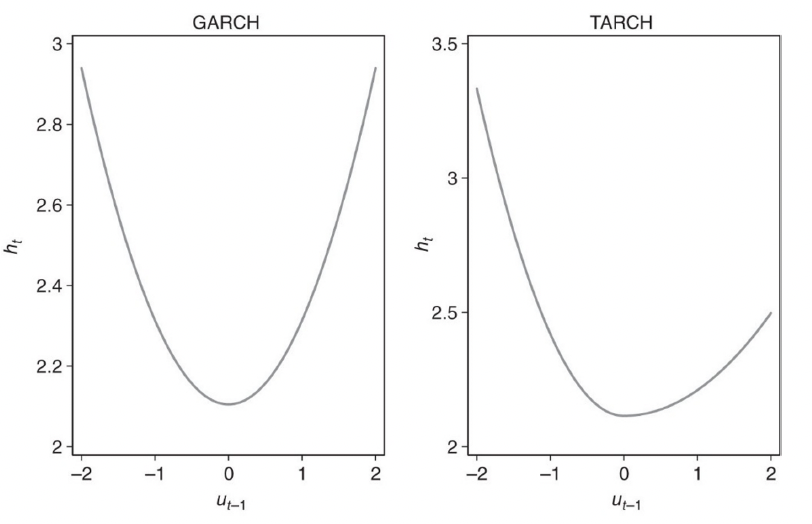
\includegraphics[width=8cm]{pics/GARCH TARCH.png}
    \caption{Comparing the Impact curves of a GARCH(1,1) to a TARCG(1,1)}
    \label{fig:GARCH TARCH}
\end{figure}

 \subsection{Forecasting with GARCH}

 Forecasts for the GARCH(1,1) model are:

 \begin{equation}
h_{T+k \mid T}= \begin{cases}\alpha_0+\alpha_1 u_T^2+\beta_1 h_T & k=1 \\ \alpha_0+\left(\alpha_1+\beta_1\right) h_{T+k-1 \mid T} & k \geqslant 2\end{cases}
\end{equation}

The conditional variance of the k-period return is then
\begin{equation}
\operatorname{var}\left(r_{T+1}(k)\right)=k \alpha_0+\alpha_1 u_T^2+\left(\left(\alpha_1+\beta_1\right)+\left(\alpha_1+\beta_1\right)^2+\cdots+\left(\alpha_1+\beta_1\right)^{k-1}\right) h_{T+1 \mid T}
\end{equation}

\begin{note}
    In practice, forecasts for the GARCH(1,1) model are done by replacing the unknown parameters $\alpha_0, \alpha_1, \beta_1$, and the unknown quantities $u_T^2$ and $h_T$, with their respective sample estimates.
\end{note}

 The forecast from a GARCH(1,1) will converge relatively quickly to the long-term average volatility implied by the model, which is given by

 \[h = \dfrac{\alpha_0}{1-\alpha_1-\beta_1}\]

 The unconditional variance $h$ is defined as long as $\alpha_1 + \beta_1 < 1$.

 \subsubsection{Accuracy of Forecasts}

 The standard method to assess volatility models is to evaluate the forecast using a volatility proxy such as the squared return, $r_t^2$.

 \paragraph{Mincer-Zarnowitz Regressions}
 a.k.a MZ regressions.
 \[h_t^2 = \delta_0 + \delta_1 \hat{h}_t + e_t\]
 where $e_t$ is a disturbance term.

 \begin{procedure}
     To test for an unbiased estimator:

     \begin{align*}
         H_0&: \delta_0 \text{ and } \delta_1 = 1 \\
         H_1&: \delta_1\neq0 \text { or } \delta_1 \neq1
     \end{align*}

     If we do \textbf{not} reject our null hypothesis, then $\hat{h}_t$ is an \textbf{unbiased estimator} of $r_t^2$.
 \end{procedure}

\begin{example}
    Adaptation of the MZ Regression:

    \begin{equation}
\begin{aligned}
\left|r_t\right| & =\delta_0+\delta_1 \sqrt{\widehat{h}_t}+e_t \\
\log r_t^2 & =\delta_0+\delta_1 \log \widehat{h}_t+e_t
\end{aligned}
\end{equation}

which use transformations of the volatility proxy to reduce the impact of large returns.
\end{example}


\subsubsection{Quasi-Likelihood}

Another approach is to use the measures of forecast performance outlined in Chapter 6 to assess volatility forecasts. There have been developments in creating new loss functions. This example is the Quasi-Likelihood loss function:
\[\text{QLIKE } = \log \hat{h}_t + \dfrac{r_t^2}{\hat{h}_t}\]

\begin{note}
    The QLIKE function can become negative when dealing with very small returns because the term in $\log h_t$ will be negative and dominate the other term in the expression.

    To avoid this we can create a specification that is always positive:
    \[\text{QLIKE } = \dfrac{r_t^2}{\hat{h}_t} - \log \left( \dfrac{r_t^2}{\hat{h}_t}\right) - 1\]
\end{note}

The QLIKE criterion is \textbf{not symmetric}. it penalises underestimating volatility more heavily than overestimating it. This could be desirable if you are a conservative risk manager.

 \begin{figure}
     \centering
     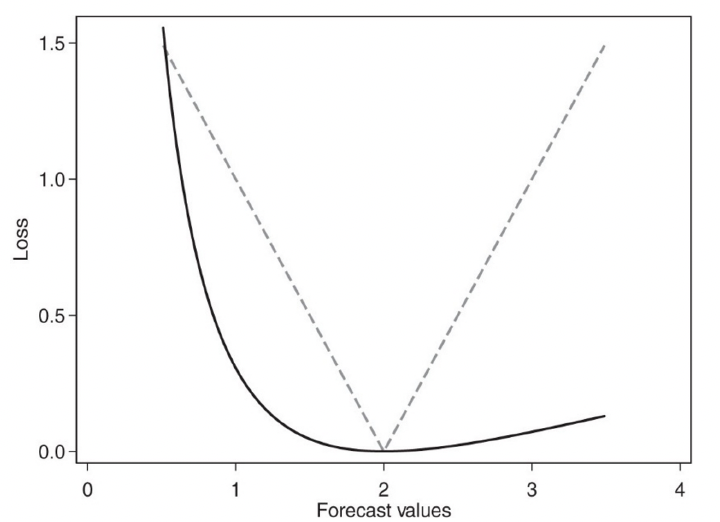
\includegraphics[width=9cm]{pics/QLIKE.png}
     \caption{Comparing the MAE (dashed) and QLIKE functions for forecast values when the hypothetical true value is 2}
     \label{fig:QLIKE}
 \end{figure}


\subsection{Applications}

\subsubsection{GARCH-M Model}

The GARCH-M model is an extension of the CAPM with an allowance for time-varying risk to identify the risk and return preference of investors. Investors must be compensated for bearing more risk (high volatility), meaning we should expect a positive relationship between the mean and the risk of the portfolio.

\begin{equation}
\begin{aligned}
r_{i t}-r_{f t} & =\mu_0+\mu_1 h_t^\omega+\mu_2\left(r_{m t}-r_{f t}\right)+u_t \\
u_t & \sim N\left(0, h_t\right) \\
h_t & =\alpha_0+\alpha_1 u_{t-1}^2+\beta_1 h_{t-1},
\end{aligned}
\end{equation}

with parameters $\theta = \{\mu_0, \mu_1, \mu_2, \alpha-0, \alpha_1, \beta_1\}$. The risk-return trade-off is given by the term $\mu_1 h_t^\omega$. When $\omega-0.5$, the risk-return trade-off is specified in terms of the conditional standard deviation. When $\omega_1$, then the relationship is expressed in terms of conditional variance.

We can test to see if there is a trade-off between risk and return:
\begin{align*}
    H_0&: \mu_1 = 0 \text{ [no trade-off]} \\
    H_1&: \mu_1 \neq0 \text{ [trade-off]}
\end{align*}

\subsubsection{Heatwaves and Meteor Showers}

An important application of GARCH models examines how volatility is transmitted through different regions of the world during the course of a global financial trading day.

An approach splits up each calendar day into three trading zones, Japan (12am-7am GMT), Europe (7am-12:30pm GMT) and the US (12:30pm-9pm GMT)

\begin{equation}
\underbrace{\overbrace{12 \mathrm{am} \cdots 7 \mathrm{am}}^{\text {Japan }}\quad \overbrace{7 \mathrm{am} \cdots 12: 30 \mathrm{pm}}^{\text {Europe }}\quad \overbrace{12: 30 \mathrm{pm} \cdots 9 \mathrm{pm}}^{\text {U.S. }}}_{\text{One Trading Day}}
\end{equation}

Define $r_1, r_2, r_3$ as the daily returns to Japanese, European and US zones respectively. The model is specified as:
\begin{equation}
    \begin{gathered}
    \left[\begin{array}{l}
r_{1 t} \\
r_{2 t} \\
r_{3 t}
\end{array}\right]=\left[\begin{array}{l}
u_{1 t} \\
u_{2 t} \\
u_{3 t}
\end{array}\right], \quad\left[\begin{array}{l}
u_{1 t} \\
u_{2 t} \\
u_{3 t}
\end{array}\right] \sim N\left(\left[\begin{array}{l}
0 \\
0 \\
0
\end{array}\right],\left[\begin{array}{ccc}
h_{1 t} & 0 & 0 \\
0 & h_{2 t} & 0 \\
0 & 0 & h_{3 t}
\end{array}\right]\right) \\
{\left[\begin{array}{l}
h_{1 t} \\
h_{2 t} \\
h_{3 t}
\end{array}\right]=\left[\begin{array}{l}
\alpha_{10} \\
\alpha_{20} \\
\alpha_{30}
\end{array}\right] } +\left[\begin{array}{ccc}
0 & 0 & 0 \\
\alpha_{21} & 0 & 0 \\
\alpha_{31} & \alpha_{32} & 0
\end{array}\right]\left[\begin{array}{l}
u_{1 t}^2 \\
u_{2 t}^2 \\
u_{3 t}^2
\end{array}\right]+\left[\begin{array}{ccc}
\beta_{11} & 0 & 0 \\
0 & \beta_{22} & 0 \\
0 & 0 & \beta_{33}
\end{array}\right]\left[\begin{array}{c}
h_{1 t-1} \\
h_{2 t-1} \\
h_{3 t-1}
\end{array}\right] \\
+  {\left[\begin{array}{ccc}
\gamma_{11} & \gamma_{12} & \gamma_{13} \\
0 & \gamma_{22} & \gamma_{23} \\
0 & 0 & \gamma_{33}
\end{array}\right]\left[\begin{array}{l}
u_{1 t-1}^2 \\
u_{2 t-1}^2 \\
u_{3 t-1}^2
\end{array}\right] . }
\end{gathered}
\end{equation}

This structure implies that:
\begin{enumerate}
    \item Japan shocks, $u_{1t}^2$ can potentially influence volatility in Europe and the US on the same day, via the coefficients $\alpha_{21}$ and $\alpha_{31}$.
    \item News from Europe can influence the US on the same day through $\alpha_{32}$, but not Japan as the market is already closed.
    \item The shocks in the US will only be transmitted to Japan and Europe the following day with parameters $\gamma_{13}, \gamma_{23}$.
\end{enumerate}

We aim to examine international linkages in volatility between these regions and investigate in particular two patterns as possible descriptors of international volatility transmission.
\begin{definition}
\begin{itemize}
    \item \textbf{Heatwaves}: Volatility in any one region is primarily a function of the previous day's volatility in the same region, $\beta_{ii} \neq0$.

    \item \textbf{Meteor Shower}: Volatility in one region is driven primarily by volatility in the region immediately preceding it in terms of the calendar time, $\alpha_{ij}\neq0$.    
\end{itemize}    
\end{definition}

\begin{procedure}
    A technically correct implementation would be to use high-frequency data and compute returns in non-overlapping zones as:

    \begin{equation}
r_{i t}=\left(\log P_{i t}^c-\log P_{i t}^o\right) / \sqrt{n h_i}, \quad i=1,2,3
\end{equation}
in which $P_{it}^c$ is a closing price of the relevant asset price in zone $i$ n day $t$. $P_{it}^o$ is the opening price.
\end{procedure}

\begin{table}[ht]
    \centering
    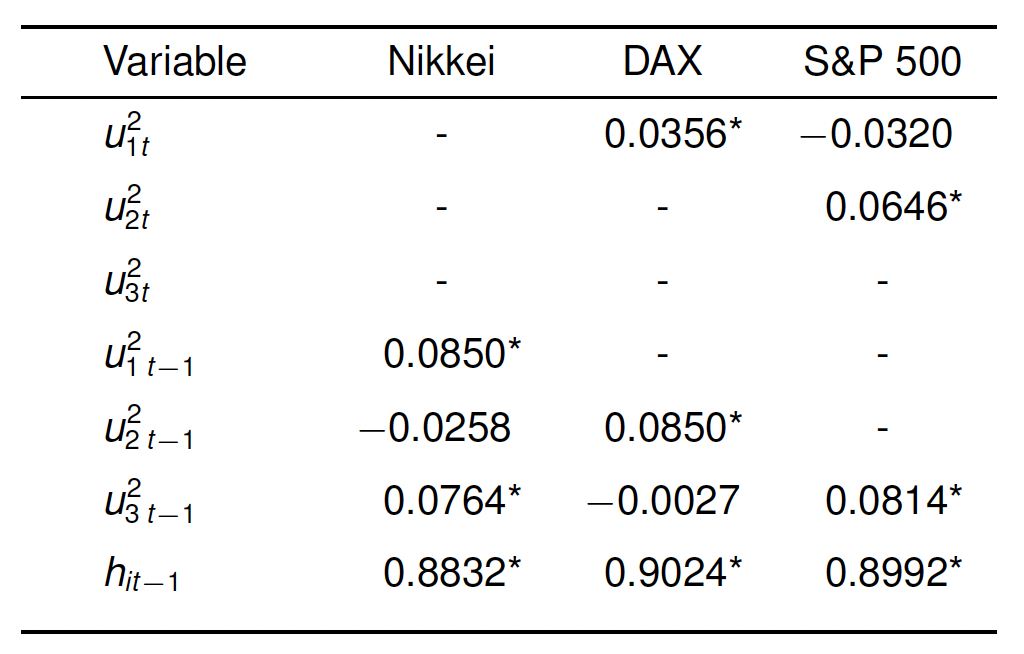
\includegraphics[width=10cm]{pics/heatwave meteor.png}
    \caption{Equation-by-equation estimation by maximum likelihood gives us this table}
    \label{tab: heatwaves and meteor showers}
\end{table}

All $h_{it-1}$ are statistically significant confirming our heat wave hypothesis. Japan affects Europe and the US on the same day; the US affects Japan the next day, confirming meteor showers.

\clearpage
\newpage
\section{Multivariate GARCH Models}
\textbf{Chapter 14}

If we want to estimate covariances, we would want to use a multivariate model. Additionally, it is important to allow covariances, to vary over time because the relationships between assets are time-varying. So, we would use a multivariate GARCH model. This allows for both variances and covariances to be time-varying.

\subsection{Motivating Examples}

\subsubsection{Time Varying Beta (CAPM)}

In our simple CAPM:
\[E[r_{it} - r_f] = \beta_i E[r_{mt}-r_f]\]

where the CAPM $\beta$ is estimated as:
\begin{equation}
\begin{aligned}
\beta & =\frac{\operatorname{cov}\left(r_{i t}-r_{f t}, r_{m t}-r_{f t}\right)}{\operatorname{var}\left(r_{m t}-r_{f t}\right)} \\
& =\frac{E\left[\left(r_{i t}-r_{f t}-E\left[r_{i t}-r_{f t}\right]\right)\left(r_{m t}-r_{f t}-\mathrm{E}\left[r_{m t}-r_{f t}\right]\right)\right]}{E\left[\left(r_{m t}-r_{f t}-\mathrm{E}\left[r_{m t}-r_{f t}\right]\right)^2\right]},
\end{aligned}
\end{equation}

The measure of $\beta$-risk is by definition constant, as it is based on the ratio of the unconditional covariance between excess market and asset returns, and the unconditional variance of the excess market returns. This constant $\beta$ is unrealistic in reality. We can respecify our $\beta_i$ in terms of conditional expectations rather than unconditional expectations. 

\begin{equation}
\beta_t=\frac{\mathrm{E}_{t-1}\left[\left(r_{i t}-r_{f t}-\mathrm{E}_{t-1}\left[r_{i t}-r_{f t}\right]\right)\left(r_{m t}-r_{f t}-\mathrm{E}_{t-1}\left[r_{m t}-r_{f t}\right]\right)\right]}{\mathrm{E}_{t-1}\left[\left(r_{m t}-r_{f t}-\mathrm{E}_{t-1}\left[r_{m t}-r_{f t}\right]\right)^2\right]},
\end{equation}

This is now a time-varying $\beta$. To use this new time-varying $\beta$, we must specify models of the conditional variance and covariance. GARCH models are able to specify time-varying conditional variance, but we need a bivariate model for estimating the time-varying conditional \textit{covariance}.

\paragraph{Estimating with OLS}

We are unable to specify
\[(r_{it}-r_{f}) = \alpha + \boldsymbol{\beta_{it}} (r_{mt}-r_f) + \epsilon_{it}\]
because we do not have enough degrees of freedom.

\subsubsection{Minimum Variance Portfolio}

If we have a portfolio with $N=2$ assets with log returns $r_{1t}, r_{2t}$. Thus, the optimal weightings of the minimum variance portfolio are
\begin{equation}
w_1=\frac{\operatorname{var}\left(r_{2 t}\right)-\operatorname{cov}\left(r_{1 t}, r_{2 t}\right)}{\operatorname{var}\left(r_{1 t}\right)+\operatorname{var}\left(r_{2 t}\right)-2 \operatorname{cov}\left(r_{1 t}, r_{2 t}\right)}
\end{equation}
where $w_2 = 1-w_1$. The optimal weights are assumed to be constant over time as they are a function of the two unconditional variances and the unconditional covariance. To relax this assumption, we can replace our unconditional expectations with conditional expectations.

\subsubsection{Value at Risk}

With our equal-weighted $N=2$ asset portfolio, the 1-day VaR is:

\[\text{VaR} = \sqrt{\text{VaR}_1^2 + \text{VaR}_2^2 + 2 \rho \text{VaR}_1\text{VaR}_2}, \]

where 
\begin{equation}
\rho=\frac{\operatorname{cov}\left(r_{1 t}, r_{2 t}\right)}{\sqrt{\operatorname{var}\left(r_{1 t}\right) \operatorname{var}\left(r_{2 t}\right)}}
\end{equation}

The maximum loss on the portfolio with a probability of 1\% is
\[\text{VaR}_i = E(r_{it}) - 2.33 \sqrt{\operatorname{var}(r_{it})}, \quad 1 = 1,2\]

Because the variances and the correlation are all unconditional measures, the VaR of the portfolio is restricted to be constant over time. We need a bivariate GARCH model to do this.

\subsection{Early Covariance Estimators}
If we have asset log returns in vector $r_t = [r_{1t} r_{2t} \ldots r_{Nt}]^\prime$. The resulting measures will be conditional sample covariance matrices.

\subsubsection{Historical Covariance}

The multivariate version of the historical estimate of the conditional covariance matrix of $r_t$ is the sample moment matrix
\begin{equation}
H_t=\frac{1}{M} \sum_{j=1}^M r_{t-j} r_{t-j}^{\prime}
\end{equation}

\begin{note}
The forecast of volatility for $k$-periods ahead is simply given by the current value $H-t$ irrespective of the value of the forecast horizon $k$.    
\end{note}

\subsubsection{Multivariate EWMA}

The multivariate version of the exponentially weighted moving average estimate of the conditional covariance matrix is
\begin{equation}
\begin{aligned}
H_t & =(1-\lambda) \sum_{j=0}^{\infty} \lambda^j r_{t-j-1} r_{t-j-1}^{\prime} \\
& =(1-\lambda) r_{t-1} r_{t-1}^{\prime}+(1-\lambda)\left[\lambda r_{t-2} r_{t-2}^{\prime}+\lambda^2 r_{t-3} r_{t-3}^{\prime}+\cdots\right] \\
& =(1-\lambda) r_{t-1} r_{t-1}^{\prime}+(1-\lambda) \lambda\left[r_{t-2} r_{t-2}^{\prime}+\lambda r_{t-3} r_{t-3}^{\prime}+\cdots\right] \\
& =(1-\lambda) r_{t-1} r_{t-1}^{\prime}+\lambda H_{t-1},
\end{aligned}
\end{equation}
where $\lambda$ is the decay parameter.

\subsubsection{Constant Correlation}

Given our equation for correlation
\begin{equation*}
\rho=\frac{\operatorname{cov}\left(r_{1 t}, r_{2 t}\right)}{\sqrt{\operatorname{var}\left(r_{1 t}\right) \operatorname{var}\left(r_{2 t}\right)}}
\end{equation*}

We can rearrange this expression to give the covariance as
\[\operatorname{cov}\left(r_{1 t}, r_{2 t}\right) = \rho \sqrt{\operatorname{var}\left(r_{1 t}\right) \operatorname{var}\left(r_{2 t}\right)}\]

This suggests that we can construct the time-varying covariance by simply replacing the unconditional variances, with their respective conditional variances based on univariate GARCH models and $\rho$ is estimated using the sample correlation coefficient.



\subsection{BEKK Model}
\begin{definition}

The multivariate GARCH model a.k.a the BEKK model is specified as:

Consider a set of $N$ log returns $r_t = [r_{1t} r_{2t} \ldots r_{Nt}]^\prime$. A time-varying estimate of the conditional covariance matrix 
\begin{equation}
H_t=\left[\begin{array}{cccc}
h_{11 t} & h_{12 t} & \cdots & h_{1 N t} \\
h_{21 t} & h_{22 t} & \cdots & h_{2 N t} \\
\vdots & \vdots & \ddots & \vdots \\
h_{N 1 t} & h_{N 2 t} & \cdots & h_{N N t}
\end{array}\right]
\end{equation}
with conditional covariances as the off-diagonal terms which satisfy the symmetry restriction $h_{ijt} = h_{jit}$. The matrix \textbf{must} be positively definite (this is a variance/covariance matrix, it wouldn't make sense for it to be negative). For a bivariate model, the conditions for positive definiteness are
\begin{equation}
    \label{conditions for positive definiteness}
    h_{11t}>0, \quad h_{11t} h_{22t} - h_{12t}^2>0
\end{equation}
\end{definition}

\subsubsection{CCC Model}

Constant Conditional Correlation Model. In the simplest 2-asset case, we have:
\begin{equation}
\left(\begin{array}{l}
r_{1, t} \\
r_{2, t}
\end{array}\right)=\left(\begin{array}{l}
u_{1 t} \\
u_{2 t}
\end{array}\right)
\end{equation}
where $u_t|I_{t-1}\sim MN(0,H_t)$ and 
\begin{equation}
H_t=\left[\begin{array}{ll}
h_{11 t} & h_{12 t} \\
h_{12 t} & h_{22 t}
\end{array}\right]
\end{equation}

The components of $H_t$ are
\begin{equation}
\left(\begin{array}{l}
h_{11 t} \\
h_{12 t} \\
h_{22 t}
\end{array}\right)=\left(\begin{array}{c}
c_{11}+a_{11} u_{1 t-1}^2+b_{11} h_{11 t-1} \\
\rho_{12} \sqrt{h_{11 t} h_{22 t}} \\
c_{22}+a_{22} u_{2 t-1}^2+b_{22} h_{22 t-1}
\end{array}\right) .
\end{equation}
\begin{note}
Even though the correlation coefficients are assumed to be constant, the covariances are time-varying.    
\end{note}
Our second condition for positive definiteness is easily satisfied, non-negativity of $h_{11t}$ requires that $c_{ii} > 0, a_{ii} \geq 0, b_{ii} \geq0$.

\subsubsection{BEKK Spec}
The BEKK specification of the conditional covariance matrix, $H_t$, is
\begin{equation}
\label{BEKK spec}
H_t = CC^\prime + A u_{t-1}u_{t-1}^\prime A^\prime + B H_{t-1} B^\prime
\end{equation}
This ensures positive definiteness of $H_t$ because coefficients are squared.

\paragraph{Asymmetric BEKK}

The parameter matrices are
\begin{equation}
C=\left[\begin{array}{cc}
c_{11} & 0 \\
c_{21} & c_{22}
\end{array}\right], \quad A=\left[\begin{array}{ll}
a_{11} & a_{12} \\
a_{21} & a_{22}
\end{array}\right], \quad B=\left[\begin{array}{ll}
b_{11} & b_{12} \\
b_{21} & b_{22}
\end{array}\right] .
\end{equation}

\paragraph{Symmetric BEKK}
\begin{equation}
C=\left[\begin{array}{cc}
c_{11} & 0 \\
c_{21} & c_{22}
\end{array}\right], \quad A=\left[\begin{array}{ll}
a_{11} & a_{12} \\
a_{12} & a_{22}
\end{array}\right], \quad B=\left[\begin{array}{ll}
b_{11} & b_{12} \\
b_{12} & b_{22}
\end{array}\right] .
\end{equation}

\paragraph{Diagonal BEKK}

\begin{equation}
C=\left[\begin{array}{cc}
c_{11} & 0 \\
c_{21} & c_{22}
\end{array}\right], \quad A=\left[\begin{array}{cc}
a_{11} & 0 \\
0 & a_{22}
\end{array}\right], \quad B=\left[\begin{array}{cc}
b_{11} & 0 \\
0 & b_{22}
\end{array}\right]
\end{equation}

\subsubsection{Estimation}

We use maximum likelihood for estimation. The log-likelihood function of a multivariate GARCH model is given by

\begin{equation}
    \label{MGARCH log likelihood function}
    \log L(\theta) = \dfrac{1}{T}\sum_{i=1}^T \log L_t = \dfrac{1}{T} \sum_{i=1}^T \log f(r_{1t}, r_{2t}, \ldots, r_{Nt};\theta),
\end{equation}
where $f(r_{1t}, r_{2t}, \ldots, r_{Nt};\theta)$ is an N-dimensional conditional multivariate probability distribution, and $\theta$ is the vector of unknown parameters. We must specify the function form of $f(r_{1t}, r_{2t}, \ldots, r_{Nt};\theta)$. There are two popular ways of doing this

\paragraph{Multivariate Normal Distribution} \mbox{}

The multivariate normal distribution is given by
\begin{equation}
f\left(r_{1 t}, r_{2 t}, \cdots, r_{N t} ; \theta\right)=\left(\frac{1}{2 \pi}\right)^{N / 2}\left|H_t\right|^{-1 / 2} \exp \left(-0.5 u_t^{\prime} H_t^{-1} u_t\right)
\end{equation}

with log-likelihood function 
\begin{equation}
\log L_t=-\frac{N}{2} \log (2 \pi)-\frac{1}{2} \log \left|H_t\right|-\frac{1}{2} u_t^{\prime} H_t^{-1} u_t
\end{equation}

\paragraph{Standardised Multivariate t distribution}

The multivariate standardised $t$ distribution is given by
\begin{equation}
f\left(r_{1 t}, r_{2 t}, \cdots, r_{N t} ; \theta\right)=\frac{\Gamma\left(\frac{\nu+N}{2}\right)}{(\pi(\nu-2))^{N / 2} \Gamma\left(\frac{\nu}{2}\right)} \times\left|H_t\right|^{-1 / 2}\left(1+\frac{u_t^{\prime} H_t^{-1} u_t}{\nu-2}\right)^{-\left(\frac{\nu+N}{2}\right)}
\end{equation}
and the log-likelihood function is
\begin{equation}
\begin{aligned}
\log L_t & =\log \Gamma\left(\frac{\nu+N}{2}\right)-\frac{N}{2} \log (\pi(\nu-2))-\log \Gamma\left(\frac{\nu}{2}\right) \\
& -\frac{1}{2} \log \left|H_t\right|-\left(\frac{\nu+N}{2}\right)\left(1+\frac{u_t^{\prime} H_t^{-1} u_t}{\nu-2}\right) .
\end{aligned}
\end{equation}

\subsection{Modelling Correlation}

One of the drawbacks of the BEKK model is that it is difficult to apply to models containing multiple assets. This is because the number of unknown parameters grows exponentially. This means that the BEKK in practice is limited to portfolios with $N<10$ assets.

\subsubsection{DCC Model}

The Dynamic Conditional Correlation (DCC) model, is a different specification which is now one of the most widely adopted MGARCH specifications in empirical work.
\begin{definition}
The DCC model is based on specifying the conditional covariance matrix as
\begin{equation}
    \label{DCC spec}
    H_t = S_t R_t S_t
\end{equation}
where $R_t$ is an $(N\times N)$ conditional correlation matrix, and $S_t$ is a diagonal matrix containing the conditional standard deviations
\begin{equation}
S_t=\left[\begin{array}{ccc}
\sqrt{h_{11 t}} & & 0 \\
& \ddots & \\
0 & & \sqrt{h_{N N t}}
\end{array}\right].
\end{equation}

\begin{note}
This is equivalent to the bivariate case in which the covariance between two assets is constructed from the product of the correlation and the two standard deviations.    
\end{note}

The \textbf{conditional variances} are of the form
\[h_{iit} = \alpha_{i0} + \alpha_{i1} u_{it-1}^2 + \beta _{i1} h_{iit-1}, \quad i =1,2,\ldots, N.\]

the \textbf{conditional correlation} matrix $R_t$ is
\begin{equation}
R_t=\operatorname{diag}\left(Q_t\right)^{-1 / 2} Q_t \operatorname{diag}\left(Q_t\right)^{-1 / 2}
\end{equation}
We express $H_t$ through a decomposition. $Q_t$ represents a pseudo-correlation matrix that has a GARCH(1,1) specification
\[Q_t = (1-\alpha-\beta) \boldsymbol{Q} + \alpha z_{t-1}z_{t-1}^\prime + \beta Q_{t-1},\]
with unknown scalar parameters $\alpha$ and $\beta$ and $z_{it} = u_{it}/\sqrt{h_{it}}$ is a standardised disturbance. The matrix $\boldsymbol{Q}$ is the unconditional second-moment matrix of standardised disturbances given by

\begin{equation}
Q=\frac{1}{T} \sum_{t=1}^T\left[\begin{array}{cccc}
z_{1 t}^2 & z_{1 t} z_{2 t} & \cdots & z_{1 t} z_{N t} \\
z_{2 t} z_{1 t} & z_{2 t}^2 & \cdots & z_{2 t} z_{N t} \\
\vdots & \vdots & \ddots & \vdots \\
z_{N t} z_{1 t} & z_{N t} z_{2 t} & \cdots & z_{N t}^2
\end{array}\right]
\end{equation}

\end{definition}

The CCC is a special case of the DCC where $\alpha=\beta=0$, resulting in $Q_t = \boldsymbol{Q}$ and $R_t = R$

\subsubsection{DCC Estimation}

\begin{procedure}
    The steps required to estimate the DCC model are:
    \begin{enumerate}
        \item Generate $h_{11t}$ and $h_{22t}$ from two univariate GARCH(1,1) models.
        \item Construct the standard deviation matrix
        \begin{equation}
            S_t=\left[\begin{array}{cc}
            \sqrt{h_{11 t}} & 0 \\
            0 & \sqrt{h_{22 t}}
        \end{array}\right]
        \end{equation}
        \item Compute the standardised residuals $z_{1t}$ and $z_{2t}$ which are then used to compute the symmetric moment matrix $\boldsymbol{Q}$.
        \item  Construct the pseudo-correlation moment matrix $Q_t$ (the one with the GARCH(1,1) specification).
        \item Compute the correlation matrix $R_t$.
        \item The resultant DCC conditional covariance matrix is

        \begin{equation}
            \begin{aligned}
            H_t & =\left[\begin{array}{cc}
            \sqrt{h_{11 t}} & 0 \\
            0 & \sqrt{h_{22 t}}
            \end{array}\right]\left[\begin{array}{cc}
            1 & \rho_{12 t} \\
            \rho_{12 t} & 1
            \end{array}\right]\left[\begin{array}{cc}
            \sqrt{h_{11 t}} & 0 \\
            0 & \sqrt{h_{22 t}}
            \end{array}\right] \\
            & =\left[\begin{array}{cc}
            h_{11 t} & \rho_{12 t} \sqrt{h_{11 t} h_{22 t}} \\
            \rho_{12 t} \sqrt{h_{11 t} h_{22 t}} & h_{22 t}
            \end{array}\right] .
            \end{aligned}
        \end{equation}
        \item Use an iterative algorithm to estimate all of the parameters simultaneously by maximising the log-likelihood function specified in terms of $H_t$.
    \end{enumerate}
\end{procedure}

\subsection{Comparing CCC, DCC, BEKK}

\paragraph{DCC} \mbox{}

Unlike BEKK, DCC does not model correlation using
\[\rho_{ij,t} = \dfrac{h_{ij,t}}{\sqrt{h_{ii,t} h_{jj,t}}}\]

rather, DDC models correlation, $R_t$, directly.

\paragraph{BEKK} \mbox{}

Practically limited to small portfolios due to the exponentially increasing number of unknown parameters.

\subsection{Dynamic Hedge Ratios}

 Multivariate GARCH models can be used to estimate dynamic hedge ratios. Consider an investor who sells futures contracts to hedge against movements in the spot price of an asset. The return on the hedged portfolio, $r_{pt}$, is
 \[r_{pt} = r_{st} - \eta r_{ft}\]

 where $s$ indicates spot market, $f$ represents futures, and $\eta$ is the number of contracts the hedger sells for each unit of spot commodity, known as the \textbf{hedge ratio}.

 The expected return and variance of the portfolio are:
 \begin{equation}
\begin{aligned}
\mu_p & =\mathrm{E}\left(r_{s t}-\eta r_{f t}\right)=\mathrm{E}\left(r_{s t}\right)-\eta \mathrm{E}\left(r_{f t}\right) \\
h_{p p} & =\mathrm{E}\left[\left(r_{p t}-\mu_p\right)^2\right]=h_{s s}+\eta^2 h_{f f}-2 \eta h_{s f}
\end{aligned}
\end{equation}

The optimal minimum variance portfolio is found by minimising $h_{pp}$ by choice of $\eta$.


\paragraph{Optimisation}

\begin{procedure}
Differentiate $h_{pp}$ wrt $\eta$, set to 0, and solve.
\begin{equation}
\frac{d h_{p p}}{d \eta}=2 \eta h_{ff}-2 h_{sf}=0 \Rightarrow \eta=\frac{h_{sf}}{h_{ff}}
\end{equation}
This gives the optimal hedge ratio, which is the ratio of the covariance of the log returns on the spot and future contracts to the variance of the returns on futures.
\end{procedure}

\paragraph{Introducing Dynamics}\mbox{}

The traditional approach is to assume the index and its futures to be perfectly correlated, but this is unrealistic. This means it may be impossible to eliminate risk and the best we can do is to minimise it.

To relax this assumption we respecify our variance and covariance terms to be time-varying. The resultant dynamic hedge ratio is then
\[\eta_t = \dfrac{h_{sft}}{h_{fft}}\]
To model the time variation in the conditional covariance, a bivariate GARCH model is required.

\paragraph{Application to US Industry Portfolios} \mbox{}

Consider the problem of hedging the log returns to the four US industry portfolios using the daily log returns and the futures contract on the S\&P 500 index. The constant hedge ratio for each industry portfolio is found by estimating the regression equation:
\begin{equation}
    \label{constant hedge ratio}
    r_{st} = \beta_0 + \beta_1 r_{ft} + u_t,
\end{equation}
where $r_{st}$ represents the log returns of to the relevant industry portfolio, $r_{ft}$ represents the log returns to the three-month S\&P 500 futures contract, and $u_t$ is the disturbance term. This gives us the constant hedge ratios of 0.773, 0.787, 1.124, and 0.768 for the consumer goods, manufacturing, technology and health portfolios.

The \textbf{dynamic hedge ratios} are computed using a bivariate dynamic conditional correlation (DCC) model specified for each industry relative to the S\&P 500 futures contract.

\begin{figure}[h]
    \centering
    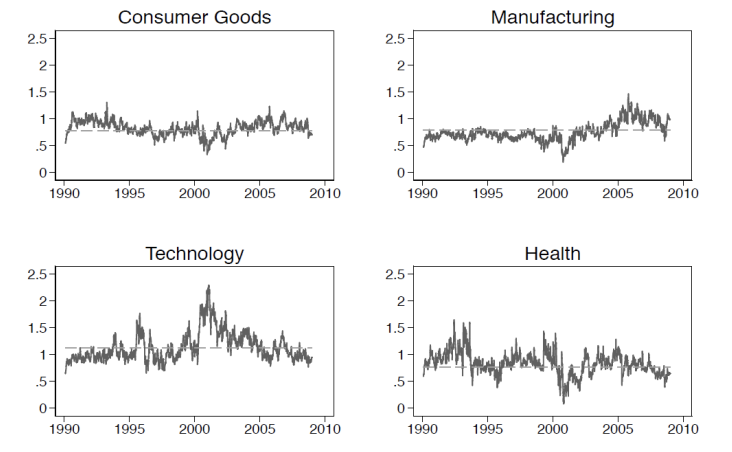
\includegraphics[width=12cm]{pics/DCC hedge ratios.png}
    \caption{Dynamic hedge Ratios for US industry Portfolios compared to the constant hedge ratio (dashed line)}
    \label{fig: dynamic hedge ratio}
\end{figure}

\newpage


\section{Stochastic Volatility}
\textbf{Chapter 12.6}
In our GARCH models, there is no randomness included in the unobserved volatility process, and it is assumed that volatility can be computed exactly based on the information set $I_{t-1}$. There is an alternative called the stochastic volatility model given by

\begin{equation}
\label{stochastic volatility}
\begin{aligned}
r_t & =\sqrt{h_t} z_t, & & z_t \sim N(0,1) \\
\log h_t & =\alpha+\phi \log h_{t-1}+v_t, & & v_t \sim N\left(0, \sigma_v^2\right),
\end{aligned}
\end{equation}

in which both $z_t$ and $v_t$ are random disturbance terms and $r_t$ represents the centred returns.

The name comes from the fact that the volatility of returns on the underlying asset is itself treated as a stochastic process. The presence of the disturbance term $v_t$ makes the variance ($h_t$) of $r_t$ a time-dependent stochastic process. There are now two random disturbances, one in returns $z_t$ and one in the variance $v_t$.

Because $h_t$ appears in both equations, the variance process is indirectly determined by disturbances in returns, and there is a potential correlation between the two source errors.

The $\sigma_v^2$ component governs the dispersion in the random component of the variance. When this variance is larger, we will have higher kurtosis. 

\section{Realised Variance and Covariance}
\textbf{Chapter 15}

\subsection{Introduction}

GARCH and stochastic volatility models treat volatility as latent/unobserved and are parametric models. With \textbf{Realised Variance}, volatility is observable and measures of realised variance are treated as observable, and a nonparametric model. It is based on observed/realised returns, hence the name.

\begin{shaded}
    At each point in time, asset price volatility is an unknown stochastic process. Once accumulated over time, this process is called the \textbf{quadratic variation}, and we want to estimate it. (it is equivalent to the time-varying conditional volatility we estimate with GARCH)

    The main idea is that we can employ very high-frequency data to ensure a nearly instantaneous focus in estimation. The precision of the variance estimates tends to increase as the sampling interval decreases (higher frequency = higher precision).
\end{shaded}

\subsection{Discrete Data}

High-frequency transaction data is not necessarily regularly spaced, unlike all the data we have seen so far. If we were looking at a binary independent variable of whether a trade has occurred, there will be clusters of many trades happening and tranquil periods.

The appropriate statistical techniques for analysing such data are expected to be different from the techniques used to analyse regularly spaced financial time series data. In a 6.5-hour trading day, the maximum number of data points is M=23400, for 1-second returns M=23400, and for 1-minute returns M=390.

To produce a sample with regularly spaced data, one approach is to fill the gaps with the last period's price/returns.

\begin{figure}[h]
    \centering
    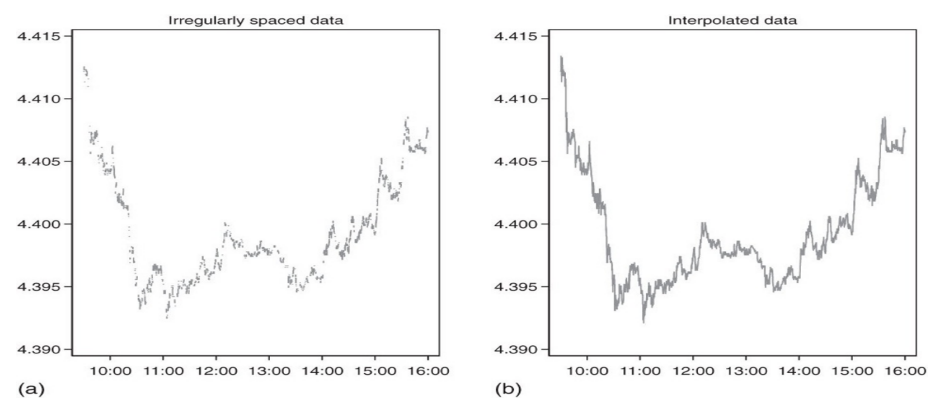
\includegraphics[width=12cm]{pics/irregular price data.png}
    \caption{Interpolating price data}
    \label{fig: fixing irregular data graph}
\end{figure}


\subsection{Realised Variance}

\begin{definition}
    Consider the log returns based on a particular sampling frequency $M$:
    \[r_i = p_{i/M} - p_{i-1/M}, \qquad i=1,2,\ldots, M.\]

    Then the realised variance for a trading day is defined as:
    \begin{equation}
        \label{Realised Variance}
        RV(M) = \sum_{i=1}^M r_i^2
    \end{equation}
\end{definition}
\newpage
\begin{figure}[h]
    \centering
    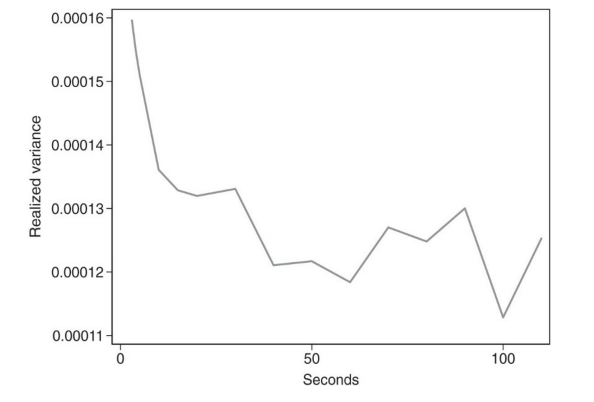
\includegraphics[width=10cm]{pics/RV signature plot.png}
    \caption{Signature plot of the estimated realised variance}
    \label{fig: RV signature}
\end{figure}

RV estimates are higher for smaller intervals and gradually decay as the sampling interval increases. Theoretically, when the intervals become infinitesimally small $M\rightarrow\infty$, we have \textbf{continuous sampling.}

The limit is known as the integrated variance, $\operatorname{plim}\sim_{i=1}^M r_i^2 = \int_{t-1}^t \sigma_s^2 ds:=IV$.

Realised variance estimates are a consistent estimator of Integrated Variance (IV).
\begin{mdframed}
    \[\operatorname{plim} RV(M) = IV\]
\end{mdframed}

\subsubsection{Integrated Variance}

So far we are looking at discrete data, but by replacing our summation operator with an integral we now look at the case of continuous sampling. So as $M\rightarrow\infty$:
\[\operatorname{plim}\sum_{i=1}^M r_i^2 = \int_{t-1}^t \sigma_s^2 ds\]
\begin{note}
    This is \textbf{exactly} the same as what I have written in the box above.
\end{note}

The sample statistic RV(M) has an asymptotic distribution
\begin{equation}
\label{initial RV(M)}
\sqrt{M} \frac{R V(M)-I V}{\sqrt{2 I Q}} \stackrel{d}{\rightarrow} N(0,1), \quad M\rightarrow\infty
\end{equation}
where the \textbf{\textit{integrated quarticity}}, IQ, is defined $IQ = \int_{t-1}^t \sigma_s^4 ds$. Our asymptotic distribution expression is very similar to the variance estimator $\hat{\sigma}^2$, which is based on sample size T of normally distributed variates with variance $\sigma^2$,

\[RV(M) = \sigma^2 = \sqrt{T}\dfrac{\hat{\sigma}^2-\sigma^2}{\sqrt{2\sigma^4}}\overset{d}{\rightarrow}N(0,1), \quad M\rightarrow\infty\]

We can approximate IQ using the realised quarticity $RQ(M) = \frac{M}{3}\sum_{i=1}^M r_i^4$. From our realised quarticity, we can find our standard errors for RV(M) as
\[se(RV) = \sqrt{\dfrac{2}{M}RQ(M)},\]
This gives us the self-normalised statistic which can be computed unlike Equation \eqref{initial RV(M)}:
\begin{equation}
    \label{RV asymptotic}
    \sqrt{M}\dfrac{RV(M) - IV}{\sqrt{2RQ(M)}}\overset{d}{\rightarrow}N(0,1), \quad M\rightarrow\infty
\end{equation}

\subsection{Microstructure Noise}

If we assume a model for log price, $p_t$, determined by a log market fundamental, $f_t$, and a random disturbance term, $u_t$, which represents microstructure noise:
\begin{equation}
    \label{microstructure initial}
    p_t = f_t + u_t
\end{equation}
we assume 
\begin{mdframed}
    \begin{align*}
        u &\sim iid(0,\sigma_u^2) \\
        u & \indep f_i     
    \end{align*}
\end{mdframed}

It can be shown that (page 445)
\[\operatorname{plim}\dfrac{RV(M)}{M} = 2\sigma_u^2,\]

which implies that as $M\rightarrow\infty$, RV is completely dominated by microstructure noise. This result is consistent with the signature plot (Figure \ref{fig: RV signature}).

\subsubsection{Dealing with Microstructure Noise}

One way to deal with this is to use 5-minute intervals (Andersen et al. 2001). Another, proposed by Zhang et al. (2005) is to use all of the information from $K$ different realised variance estimators, constructed at sparse frequencies (e.g. 5 minutes), into a unique estimator.

Let $\{M_1, M_2, \ldots, M_k\}$ represent the sparse frequencies. The new RV estimate is
\begin{equation}
\label{RV ZMA}
R V_{Z M A}=\frac{1}{K} \sum_{k=1}^K R V_k\left(M_k\right)-\frac{\bar{M}}{M} R V(M)
\end{equation}
where $\bar{M} = \frac{1}{K}\sum_{k=1}^K M_k$ is the sample average of the sparse sampling frequencies.

\paragraph{Choosing K} \mbox{}

The choice of K (our number of estimators combined to create a new RV value), is determined by
\[\left(\dfrac{RQ}{12(\hat{\sigma}_u^2)^2}\right)^{-1/3} M^{2/1},\]
where $\hat{\sigma}_u^2 = \frac{1}{2M}\sum_{i=1}^M r_i^2$.

\subsection{HAR Model}
The HAR model uses the daily time series of realised variance to forecast movements in volatility. Let $RV_t^{(d)}$ represent the daily RV at day $t$. We can construct weekly, monthly etc. values:

\begin{equation}
\begin{array}{ll}
\text { Weekly } & : \quad R V_t^{(w)}=\frac{1}{5}\left(R V_t^{(d)}+R V_{t-1}^{(d)}+\cdots+R V_{t-4}^{(d)}\right) \\
\text { Monthly } & : \quad R V_t^{(m)}=\frac{1}{22}\left(R V_t^{(d)}+R V_{t-1}^{(d)}+\cdots+R V_{t-21}^{(d)}\right)
\end{array}
\end{equation}

\begin{definition}
    The HAR model is specified as the following autoregressive model:
    \begin{equation}
    \label{HAR}
R V_t^{(d)}=\beta_0+\beta_d R V_{t-1}^{(d)}+\beta_w R V_{t-1}^{(w)}+\beta_m R V_{t-1}^{(m)}+u_t
\end{equation}
where $u_t$ is a disturbance term. Tomorrows variance is a function of three components (which capture the role of heterogenous traders)
\begin{itemize}
    \item $RV_t^{(d)}$ captures daily or high frequency traders
    \item $RV_t^{(w)}$ captures investors who typically re-balance their positions weekly
    \item $RV_t^{(m)}$ captures relatively long-term investors with investment horizons of one month or longer.
\end{itemize}
The HAR model is a restricted AR(22) model with only 4 parameters $\{\beta_0, \beta_d, \beta_w \beta_m\}$. 
\end{definition}

\begin{figure}[h]
    \centering
    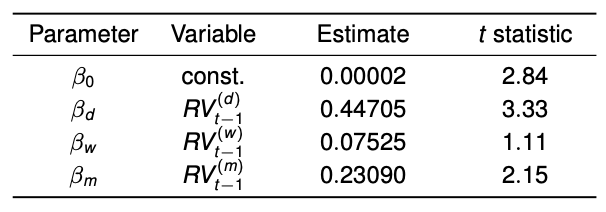
\includegraphics[width=9cm]{pics/HAR results.png}
    \caption{Results from running the OLS of our HAR model}
    \label{fig:mHAR results}
\end{figure}

Our results tell us that our parameter estimate associated with the weekly variance estimator is not statistically significant. To examine our HAR model, we can find MSE, MAE, QLIKE to compare to just the individual aspects of the model

\begin{figure}[h]
    \centering
    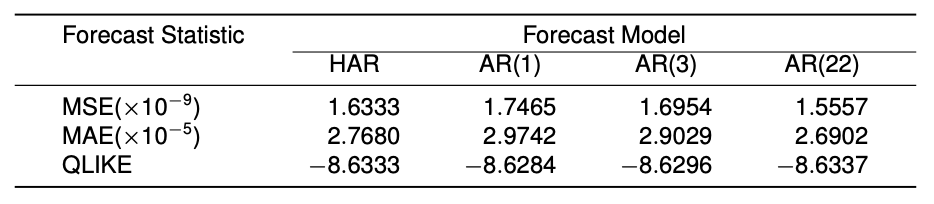
\includegraphics[width=12cm]{pics/HAR measurement stats.png}
    \caption{Comparative statistics of the HAR model}
    \label{fig:HAR compare}
\end{figure}
\begin{note}
    That should be an AR(5) model, it is the weekly estimate.
\end{note}

We can see that the HAR model outperforms the AR(1) and the AR(5), but not the AR(22). This tells us that the restrictions imposed on the lag structure of the HAR model are not necessarily consistent with the data.

\subsection{Realised GARCH}

Hansen (2012) proposed a realised GARCH model by augmenting the GARCH specification with the conditional variance $h_t$ representing IV.

\begin{definition}
We specify our model as:
    \begin{equation}
    \label{Realised GARCH}
\begin{aligned}
r_t & =\mu_0+u_t \\
h_t & =\alpha_0+\alpha_1 R V_{t-1}+\beta_1 h_{t-1} \\
R V_t & =\delta_0+\delta_1 h_t+v_t \\
u_t & \sim N\left(0, h_t\right), \quad v_t \sim N\left(0, \sigma_v^2\right) .
\end{aligned}
\end{equation}
The model is a bivariate model with dependent variables $r_t$ and $RV_t$. The log-likelihood function if the realised GARCH model is
\begin{equation}
\begin{aligned}
\log L(\theta)&=-\frac{1}{2 T} \sum_{t=1}^T\left(\log (2 \pi)+\log \left(h_t\right)+\frac{r_t^2}{h_t}\right) \\
&-\frac{1}{2 T} \sum_{t=1}^T\left(\log (2 \pi)+\log \left(\sigma_v^2\right)+\frac{\left(R V_t-\delta_0-\delta_1 h_t\right)^2}{\sigma_v^2}\right) \\
&= \log L_1(\theta_1) + \log L_2 (\theta_1, \theta_2).
\end{aligned}
\end{equation}

The term $\log L_1(\theta_1)$ represents the log-likelihood function of the standard GARCH model, and $\log L_2 (\theta_1, \theta_2)$ represents the log-likelihood of the $RV_t$.
\end{definition}
\newpage

\begin{figure}[h]
    \centering
    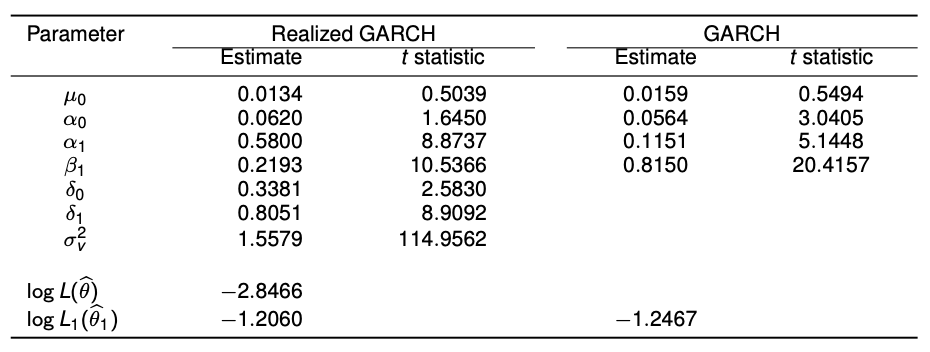
\includegraphics{pics/realised GARCH vs GARCH.png}
    \caption{Comparing the results of GARCH and Realised GARCH}
    \label{fig: GARCH vs Realised GARCH}
\end{figure}

We can see here, that the realised GARCH model performs better than the normal GARCH model.
\begin{enumerate}
    \item Our partial log-likelihood function $\log L_1(\theta_1)$ is larger
    \item Our $\alpha_1$ parameter is much greater (5 times larger) and more significant
    \item Our $\delta_1$ coefficient is statistically significant which indicates a strong relationship between integrated volatility $h_t$ and realised volatility $RV_t$.
\end{enumerate}

\subsection{Realised Covariance}

So far we have looked at univariate models of realised variance. In our MGARCH models, our analysis extends to $N$ assets to allow for variances \textbf{and covariances}. We want to do the same with realised covariances.

In the case of 2 assets, sampled at $M$ intervals a day, the realised covariance for a day is

\begin{equation}
\label{realised covariance}
R C(M)=\left(\begin{array}{cc}
\sum_{i=1}^M r_{1 i}^2 & \sum_{i=1}^M r_{1 i} r_{2 i} \\
\sum_{i=1}^M r_{2 i} r_{1 i} & \sum_{i=1}^M r_{2 i}^2
\end{array}\right)
\end{equation}

The realised covariance matric is a consistent estimator of the \textbf{\textit{integrated covariance}}, that is, as $M\rightarrow\infty$, 
\[\operatorname{plim}RC(M) \rightarrow IC\]

where
\begin{equation}
\label{integrated covariance}
I C=\left(\begin{array}{cc}
\int_{t-1}^t \sigma_{1 s}^2 d s & \int_{t-1}^t \sigma_{1 s} \sigma_{2 s} d s \\
\int_{t-1}^t \sigma_{1 s} \sigma_{2 s} d s & \int_{t-1}^t \sigma_{2 s}^2 d s
\end{array}\right)
\end{equation}

\begin{note}
    The presence of microstructure noise can distort estimates based on realised covariances. Also, when working with high-frequency multivariate data, because financial assets are commonly traded at different time stamps we are subject to the \textbf{Epps Effect}.
\end{note}

\subsection{Epps Effect}

Epps (1979) showed that the effect of non-synchronous trading leads to a \textbf{downward bias of the realised covariance estimator}.

To do this, we simulate the following discretised bivariate stochastic differential system

\begin{equation}
\label{Epps model}
p_{i / M}=p_{(i-1) / M}+\mu \Delta t+\Omega^{1 / 2} \Delta B_{i / M}, \quad i=1,2, \cdots, 23400
\end{equation}

where the elements are defined as:
\begin{equation}
\begin{aligned}
\mu & =\left[\begin{array}{l}
0.05 \\
0.05
\end{array}\right] \frac{1}{250}=\left[\begin{array}{l}
2 \times 10^{-4} \\
2 \times 10^{-4}
\end{array}\right], \\
\Omega & =\left[\begin{array}{ll}
0.04 & 0.03 \\
0.03 & 0.05
\end{array}\right] \frac{1}{250}=\left[\begin{array}{ll}
1.6 \times 10^{-4} & 1.2 \times 10^{-4} \\
1.2 \times 10^{-4} & 2.0 \times 10^{-4}
\end{array}\right],
\end{aligned}
\end{equation}
and $\Delta B_{i/M}$ is a bivariate normal random variable distributed as $N(0,\Delta t)$

\begin{figure}[h]
    \centering
    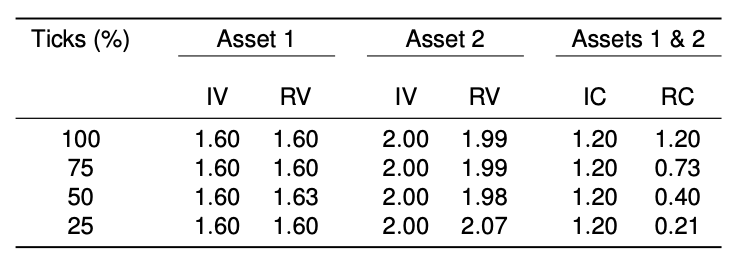
\includegraphics{pics/simulated Epps.png}
    \caption{Results from Simulating our Epps model from Equation \eqref{Epps model}}
    \label{fig:epps results}
\end{figure}

When the number of active traders is reduced to 75\%, the realised variances exhibit no bias, but the realised covariance is now biased downward. This bias only continues to increase in the presence of more non-synchronous trading.
\begin{note}
    RC is our estimate for IC, so the difference is the bias we are referring to.
\end{note}

\subsubsection{Correcting for the Epps Effect}

To correct for the Epps effect we can implement a sampling scheme that generates synchronised prices across assets, known as the \textbf{refresh time synchronisation scheme}.

\begin{procedure}
    The first refresh time, $\tau(1)$, is the first time since the opening of the market when all assets have traded \textbf{at least once.} The refresh prices are then the current or the recent prices of the assets.

    The second refresh time is the next time all assets have been traded at least once since the refresh time $\tau(1)$.

    Repeating this sequence yields in total $M$ refresh times, $\tau(j), j = 1,2, \ldots, M$, and corresponding $M$ sets of synchronised refresh prices $p_{\tau(j)}$.
\end{procedure}

\begin{figure}[h]
    \centering
    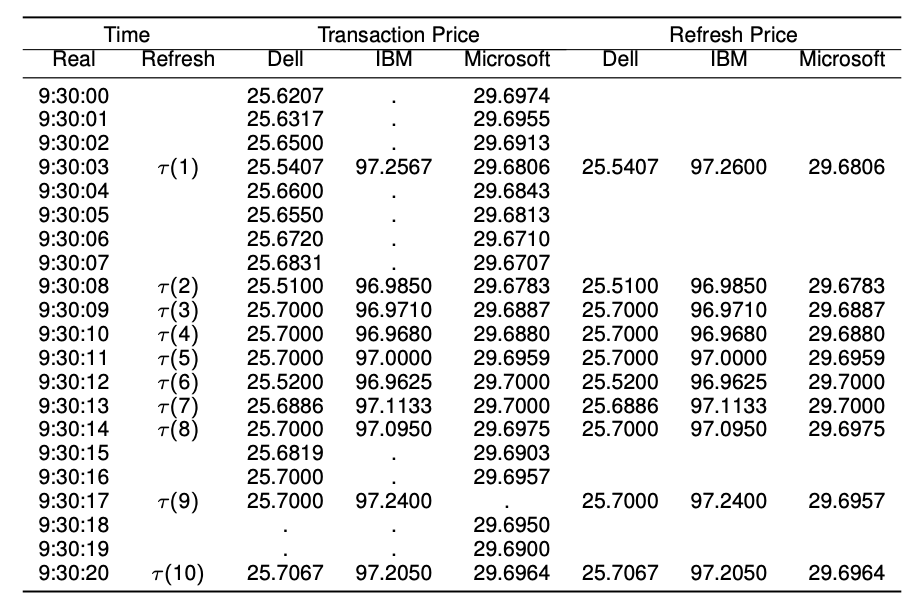
\includegraphics[width=12cm]{pics/refresh times.png}
    \caption{Refresh times for Dell IBM Microsoft in the first 20 seconds of the trading day}
    \label{fig:refresh times}
\end{figure}

Once the refresh times have been established, the intra-day log returns are computed using the refresh prices, When $M\rightarrow\infty$ and there is no microstructure noise, $\operatorname{plim} RC(M) \rightarrow IC$.To see the microstructure noise at relatively high frequencies, signature plots for RV and RC may be used.

\begin{figure}[h]
    \centering
    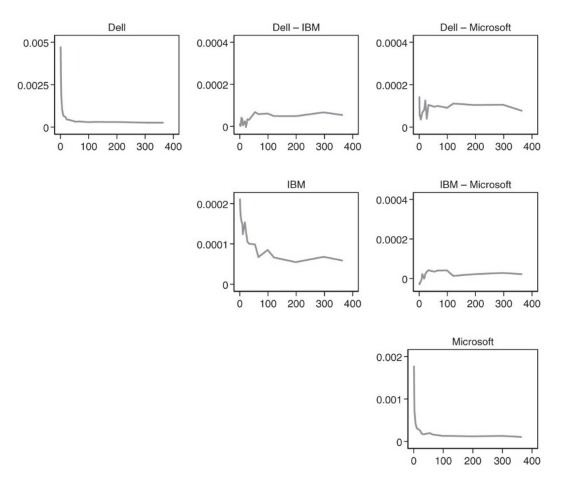
\includegraphics[width=8cm]{pics/refresh signature plots.png}
    \caption{RV and RC of Dell IBM and Microsoft}
    \label{fig:refresh rate covariance signature plots}
\end{figure}

The realised covariance matrix for Dell, IBM and Microsoft using all $M=6535$ refreshed log returns is:

\begin{equation}
R C=\left(\begin{array}{rrr}
469.90 \times 10^{-5} & 1.12 \times 10^{-5} & 14.16 \times 10^{-5} \\
1.12 \times 10^{-5} & 21.00 \times 10^{-5} & -2.90 \times 10^{-5} \\
14.16 \times 10^{-5} & -2.90 \times 10^{-5} & 176.70 \times 10^{-5}
\end{array}\right)
\end{equation}

For all three stocks, the RV and RC stabilise if 54 or fewer refresh log returns are used. the full RC matrix based on 54 refresh log returns is
\begin{equation}
R C(54)=\left(\begin{array}{rrr}
30.9 \times 10^{-5} & 4.90 \times 10^{-5} & 1.36 \times 10^{-5} \\
4.90 \times 10^{-5} & 6.65 \times 10^{-5} & 11.10 \times 10^{-5} \\
1.36 \times 10^{-5} & 11.10 \times 10^{-5} & 13.20 \times 10^{-5}
\end{array}\right)
\end{equation}









\end{document}